\documentclass[twoside]{book}

% Packages required by doxygen
\usepackage{fixltx2e}
\usepackage{calc}
\usepackage{doxygen}
\usepackage[export]{adjustbox} % also loads graphicx
\usepackage{graphicx}
\usepackage[utf8]{inputenc}
\usepackage{makeidx}
\usepackage{multicol}
\usepackage{multirow}
\PassOptionsToPackage{warn}{textcomp}
\usepackage{textcomp}
\usepackage[nointegrals]{wasysym}
\usepackage[table]{xcolor}

% Font selection
\usepackage[T1]{fontenc}
\usepackage[scaled=.90]{helvet}
\usepackage{courier}
\usepackage{amssymb}
\usepackage{sectsty}
\renewcommand{\familydefault}{\sfdefault}
\allsectionsfont{%
  \fontseries{bc}\selectfont%
  \color{darkgray}%
}
\renewcommand{\DoxyLabelFont}{%
  \fontseries{bc}\selectfont%
  \color{darkgray}%
}
\newcommand{\+}{\discretionary{\mbox{\scriptsize$\hookleftarrow$}}{}{}}

% Page & text layout
\usepackage{geometry}
\geometry{%
  a4paper,%
  top=2.5cm,%
  bottom=2.5cm,%
  left=2.5cm,%
  right=2.5cm%
}
\tolerance=750
\hfuzz=15pt
\hbadness=750
\setlength{\emergencystretch}{15pt}
\setlength{\parindent}{0cm}
\setlength{\parskip}{3ex plus 2ex minus 2ex}
\makeatletter
\renewcommand{\paragraph}{%
  \@startsection{paragraph}{4}{0ex}{-1.0ex}{1.0ex}{%
    \normalfont\normalsize\bfseries\SS@parafont%
  }%
}
\renewcommand{\subparagraph}{%
  \@startsection{subparagraph}{5}{0ex}{-1.0ex}{1.0ex}{%
    \normalfont\normalsize\bfseries\SS@subparafont%
  }%
}
\makeatother

% Headers & footers
\usepackage{fancyhdr}
\pagestyle{fancyplain}
\fancyhead[LE]{\fancyplain{}{\bfseries\thepage}}
\fancyhead[CE]{\fancyplain{}{}}
\fancyhead[RE]{\fancyplain{}{\bfseries\leftmark}}
\fancyhead[LO]{\fancyplain{}{\bfseries\rightmark}}
\fancyhead[CO]{\fancyplain{}{}}
\fancyhead[RO]{\fancyplain{}{\bfseries\thepage}}
\fancyfoot[LE]{\fancyplain{}{}}
\fancyfoot[CE]{\fancyplain{}{}}
\fancyfoot[RE]{\fancyplain{}{\bfseries\scriptsize Generated by Doxygen }}
\fancyfoot[LO]{\fancyplain{}{\bfseries\scriptsize Generated by Doxygen }}
\fancyfoot[CO]{\fancyplain{}{}}
\fancyfoot[RO]{\fancyplain{}{}}
\renewcommand{\footrulewidth}{0.4pt}
\renewcommand{\chaptermark}[1]{%
  \markboth{#1}{}%
}
\renewcommand{\sectionmark}[1]{%
  \markright{\thesection\ #1}%
}

% Indices & bibliography
\usepackage{natbib}
\usepackage[titles]{tocloft}
\setcounter{tocdepth}{3}
\setcounter{secnumdepth}{5}
\makeindex

% Hyperlinks (required, but should be loaded last)
\usepackage{ifpdf}
\ifpdf
  \usepackage[pdftex,pagebackref=true]{hyperref}
\else
  \usepackage[ps2pdf,pagebackref=true]{hyperref}
\fi
\hypersetup{%
  colorlinks=true,%
  linkcolor=blue,%
  citecolor=blue,%
  unicode%
}

% Custom commands
\newcommand{\clearemptydoublepage}{%
  \newpage{\pagestyle{empty}\cleardoublepage}%
}

\usepackage{caption}
\captionsetup{labelsep=space,justification=centering,font={bf},singlelinecheck=off,skip=4pt,position=top}

%===== C O N T E N T S =====

\begin{document}

% Titlepage & ToC
\hypersetup{pageanchor=false,
             bookmarksnumbered=true,
             pdfencoding=unicode
            }
\pagenumbering{roman}
\begin{titlepage}
\vspace*{7cm}
\begin{center}%
{\Large Labor Embedded Software }\\
\vspace*{1cm}
{\large Generated by Doxygen 1.8.11}\\
\end{center}
\end{titlepage}
\clearemptydoublepage
\tableofcontents
\clearemptydoublepage
\pagenumbering{arabic}
\hypersetup{pageanchor=true}

%--- Begin generated contents ---
\chapter{Author\+: Rafiqul Islam}
\label{index}\hypertarget{index}{}\section*{Architecture }

In this project, I implement 3 layers of Rasp\+Net protocol. Rasp\+Net is a networking protocol contains 7 layers as like as O\+SI model, but limited to basic functions. In this project, I developed \+Physical Layer, Data Link Layer and Network Layer of Rasp\+Net protocol. \subsection*{Physical Layer}

This layer is responsible for sending and receiving raw bit streams over the physical medium. According to, Rasp\+Net protocol, in Physical Layer two wires are used from one node to the next. The first one is data-\/pin, the second one is the clock-\/signal. Whenever the clock-\/signal changes (from 1 to 0 or from 0 to 1) there is a new bit there for reading on the data-\/pin. \subsection*{Data Link Layer}

This layer is responsible for the reliable transmission of data frames between two connected nodes. According to Rasp\+Net, Layer 2 bundles all bits together to send network frames. A network frame begins with a preamble of \char`\"{}01111110\char`\"{}. In this layer, C\+R\+C-\/32 (cyclic redundancy check) is used for error detection. \subsection*{Network Layer}

This layer structure and manage a multi-\/node network, addressing, routing as well as traffic control. According to Rasp\+Net protocol, Layer 3 handles addressing, routing as well as the priority of each packet.\+ 

\section*{Technology }

\subsection*{Programming language}

C programming language is used to implement this Rasp\+Net protocol.

\subsection*{Hardware device}


\begin{DoxyItemize}
\item Raspberry Pi\+: Raspberry pi is a single-\/board computer.
\item Gertboard\+: \+The Gertboard is an input/output (I/O) extension board for the Raspberry Pi computer. It fits onto the\+G\+P\+IO (general-\/purpose Input/\+Output) pins of the Raspberry Pi.\+ 
\item Microcontroller\+: A\+VR Atmega328p microcontroller is used here. Gertboard contains this microcontroller inside the board. So it is not needed to add a separate microcontroller. Atmega328p is a single-\/chip microcontroller. It has an 8 bit R\+I\+SC processor.
\end{DoxyItemize}

\subsection*{Toolchain}


\begin{DoxyItemize}
\item Operating system\+: Linux based operating system is used here. N\+O\+OB, Raspbian, R\+I\+SC OS, \+Ubuntu Mate, Ubuntu Core, etc are usually used for Raspberry Pi computer.
\item Serial communication program\+: For serial communication purposes, minicom is used. Minicom is a text-\/based serial communication program. Minicom command from the terminal has been given below.
\end{DoxyItemize}

\begin{quote}
{\bfseries Command\+:} minicom -\/b 19200 -\/o -\/D /dev/tty\+A\+M\+A0 \end{quote}



\begin{DoxyItemize}
\item Compiler\+: avr-\/gcc is used to compile C code.
\item avrdude\+: A\+V\+R\+D\+U\+DE is a command line program to download/upload/manipulate the R\+OM and E\+E\+P\+R\+OM contents of A\+VR microcontrollers using the in-\/system programming techniquee.
\item Compiler\+:gcc-\/avr \+: Cross-\/compiler for C programming complitation for A\+VR microcontroller.
\item A\+VR library\+: avr-\/libc library is used which provides built-\/in functionalities to use with C programming.
\end{DoxyItemize}

\subsection*{Installation}


\begin{DoxyItemize}
\item Minicom installation in Linux (Debian, Ubuntu, Kali, Mint) \begin{quote}
{\bfseries Command\+:} sudo apt install minicom -\/y \end{quote}

\item Minicom installation in Linux (Fedora, Cent\+OS, R\+H\+EL) \begin{quote}
{\bfseries Command\+:} sudo yum install minicom -\/y \end{quote}

\item avrdude installation in Linux \begin{quote}
{\bfseries Command\+:} sudo apt-\/get install avrdude \end{quote}

\item A\+VR tool chain installation\+: \begin{quote}
{\bfseries Command\+:} sudo apt-\/get install gcc-\/avr binutils-\/avr avr-\/libc \end{quote}

\end{DoxyItemize}

\subsection*{Reference Links\+:}


\begin{DoxyItemize}
\item \mbox{[} Rasp\+Net protocol \mbox{]}\+: \mbox{[} \href{https://osg.informatik.tu-chemnitz.de/lehre/emblab/protocol_final_4stud.pdf}{\tt https\+://osg.\+informatik.\+tu-\/chemnitz.\+de/lehre/emblab/protocol\+\_\+final\+\_\+4stud.\+pdf} \mbox{]}
\item \mbox{[}Gertboard Manual\mbox{]}\+: \mbox{[} \href{https://osg.informatik.tu-chemnitz.de/lehre/emblab/gertboard_manual_2.0.pdf}{\tt https\+://osg.\+informatik.\+tu-\/chemnitz.\+de/lehre/emblab/gertboard\+\_\+manual\+\_\+2.\+0.\+pdf} \mbox{]}
\item \mbox{[}A\+VR\mbox{]}\+: \mbox{[} \href{https://osg.informatik.tu-chemnitz.de/lehre/emblab/atmel.pdf}{\tt https\+://osg.\+informatik.\+tu-\/chemnitz.\+de/lehre/emblab/atmel.\+pdf} \mbox{]}
\item \mbox{[}avrdude\mbox{]}\+: \mbox{[}\href{https://www.nongnu.org/avrdude/}{\tt https\+://www.\+nongnu.\+org/avrdude/} \mbox{]}
\item \mbox{[}avr-\/gcc\mbox{]}\+: \mbox{[}\href{https://gcc.gnu.org/wiki/avr-gcc}{\tt https\+://gcc.\+gnu.\+org/wiki/avr-\/gcc} \mbox{]}
\item \mbox{[}Minicom\mbox{]}\+: \mbox{[}\href{https://salsa.debian.org/minicom-team/minicom5}{\tt https\+://salsa.\+debian.\+org/minicom-\/team/minicom5} \mbox{]}
\item \mbox{[}Raspberry Pi\mbox{]}\+: \mbox{[}\href{https://www.raspberrypi.org/}{\tt https\+://www.\+raspberrypi.\+org/} \mbox{]} 
\end{DoxyItemize}
\chapter{Class Index}
\section{Class List}
Here are the classes, structs, unions and interfaces with brief descriptions\+:\begin{DoxyCompactList}
\item\contentsline{section}{\hyperlink{structPacket}{Packet} }{\pageref{structPacket}}{}
\end{DoxyCompactList}

\chapter{File Index}
\section{File List}
Here is a list of all files with brief descriptions\+:\begin{DoxyCompactList}
\item\contentsline{section}{Rasp\+Net/\+C\+R\+C calculation/\hyperlink{CRC_8c}{C\+R\+C.\+c} }{\pageref{CRC_8c}}{}
\item\contentsline{section}{Rasp\+Net/\+C\+R\+C calculation/\hyperlink{CRC_8h}{C\+R\+C.\+h} }{\pageref{CRC_8h}}{}
\item\contentsline{section}{Rasp\+Net/\+Interrupt Handler/\hyperlink{PIN__Change__Interrupt__Handler_8c}{P\+I\+N\+\_\+\+Change\+\_\+\+Interrupt\+\_\+\+Handler.\+c} }{\pageref{PIN__Change__Interrupt__Handler_8c}}{}
\item\contentsline{section}{Rasp\+Net/\+Interrupt Handler/\hyperlink{Timer__Interrupt__Handler_8c}{Timer\+\_\+\+Interrupt\+\_\+\+Handler.\+c} }{\pageref{Timer__Interrupt__Handler_8c}}{}
\item\contentsline{section}{Rasp\+Net/\+Layer 1/\hyperlink{Layer1_8c}{Layer1.\+c} }{\pageref{Layer1_8c}}{}
\item\contentsline{section}{Rasp\+Net/\+Layer 1/\hyperlink{Layer1_8h}{Layer1.\+h} }{\pageref{Layer1_8h}}{}
\item\contentsline{section}{Rasp\+Net/\+Layer 2/\hyperlink{Layer2_8c}{Layer2.\+c} }{\pageref{Layer2_8c}}{}
\item\contentsline{section}{Rasp\+Net/\+Layer 2/\hyperlink{Layer2_8h}{Layer2.\+h} }{\pageref{Layer2_8h}}{}
\item\contentsline{section}{Rasp\+Net/\+Layer 3/\hyperlink{Layer3_8c}{Layer3.\+c} }{\pageref{Layer3_8c}}{}
\item\contentsline{section}{Rasp\+Net/\+Layer 3/\hyperlink{Layer3_8h}{Layer3.\+h} }{\pageref{Layer3_8h}}{}
\item\contentsline{section}{Rasp\+Net/\+Main and Others/\hyperlink{Buffer_8c}{Buffer.\+c} }{\pageref{Buffer_8c}}{}
\item\contentsline{section}{Rasp\+Net/\+Main and Others/\hyperlink{initialization_8c}{initialization.\+c} }{\pageref{initialization_8c}}{}
\item\contentsline{section}{Rasp\+Net/\+Main and Others/\hyperlink{initialization_8h}{initialization.\+h} }{\pageref{initialization_8h}}{}
\item\contentsline{section}{Rasp\+Net/\+Main and Others/\hyperlink{main_8c}{main.\+c} }{\pageref{main_8c}}{}
\item\contentsline{section}{Rasp\+Net/\+Main and Others/\hyperlink{Miscellaneous_8c}{Miscellaneous.\+c} }{\pageref{Miscellaneous_8c}}{}
\item\contentsline{section}{Rasp\+Net/\+Main and Others/\hyperlink{Miscellaneous_8h}{Miscellaneous.\+h} }{\pageref{Miscellaneous_8h}}{}
\item\contentsline{section}{Rasp\+Net/\+U\+A\+R\+T handler/\hyperlink{UART__Handler_8c}{U\+A\+R\+T\+\_\+\+Handler.\+c} }{\pageref{UART__Handler_8c}}{}
\item\contentsline{section}{Rasp\+Net/\+U\+A\+R\+T handler/\hyperlink{UART__Handler_8h}{U\+A\+R\+T\+\_\+\+Handler.\+h} }{\pageref{UART__Handler_8h}}{}
\end{DoxyCompactList}

\chapter{Class Documentation}
\hypertarget{structPacket}{}\section{Packet Struct Reference}
\label{structPacket}\index{Packet@{Packet}}
\subsection*{Public Attributes}
\begin{DoxyCompactItemize}
\item 
uint8\+\_\+t \hyperlink{structPacket_af626fe07d93fe4116d613304792df080}{destination}
\item 
uint8\+\_\+t \hyperlink{structPacket_a01308f5b690e5060fea6037e765058b9}{source}
\item 
uint8\+\_\+t \hyperlink{structPacket_aa305c88136c91911a5159610863cb41d}{preamble}
\item 
uint32\+\_\+t \hyperlink{structPacket_abad95795e9615463d9d69d298a86b0b8}{crc}
\item 
uint8\+\_\+t \hyperlink{structPacket_ab13014675ea9eda122b1c50842a567fc}{payload\+\_\+siz}
\item 
uint8\+\_\+t \hyperlink{structPacket_a58a48ac639979f488f254bbcb98e72b8}{payload} \mbox{[}250\mbox{]}
\end{DoxyCompactItemize}


\subsection{Member Data Documentation}
\index{Packet@{Packet}!crc@{crc}}
\index{crc@{crc}!Packet@{Packet}}
\subsubsection[{\texorpdfstring{crc}{crc}}]{\setlength{\rightskip}{0pt plus 5cm}uint32\+\_\+t Packet\+::crc}\hypertarget{structPacket_abad95795e9615463d9d69d298a86b0b8}{}\label{structPacket_abad95795e9615463d9d69d298a86b0b8}
Store C\+RC \index{Packet@{Packet}!destination@{destination}}
\index{destination@{destination}!Packet@{Packet}}
\subsubsection[{\texorpdfstring{destination}{destination}}]{\setlength{\rightskip}{0pt plus 5cm}uint8\+\_\+t Packet\+::destination}\hypertarget{structPacket_af626fe07d93fe4116d613304792df080}{}\label{structPacket_af626fe07d93fe4116d613304792df080}
Store destination address \index{Packet@{Packet}!payload@{payload}}
\index{payload@{payload}!Packet@{Packet}}
\subsubsection[{\texorpdfstring{payload}{payload}}]{\setlength{\rightskip}{0pt plus 5cm}uint8\+\_\+t Packet\+::payload\mbox{[}250\mbox{]}}\hypertarget{structPacket_a58a48ac639979f488f254bbcb98e72b8}{}\label{structPacket_a58a48ac639979f488f254bbcb98e72b8}
Store payload \index{Packet@{Packet}!payload\+\_\+siz@{payload\+\_\+siz}}
\index{payload\+\_\+siz@{payload\+\_\+siz}!Packet@{Packet}}
\subsubsection[{\texorpdfstring{payload\+\_\+siz}{payload_siz}}]{\setlength{\rightskip}{0pt plus 5cm}uint8\+\_\+t Packet\+::payload\+\_\+siz}\hypertarget{structPacket_ab13014675ea9eda122b1c50842a567fc}{}\label{structPacket_ab13014675ea9eda122b1c50842a567fc}
Store payload size \index{Packet@{Packet}!preamble@{preamble}}
\index{preamble@{preamble}!Packet@{Packet}}
\subsubsection[{\texorpdfstring{preamble}{preamble}}]{\setlength{\rightskip}{0pt plus 5cm}uint8\+\_\+t Packet\+::preamble}\hypertarget{structPacket_aa305c88136c91911a5159610863cb41d}{}\label{structPacket_aa305c88136c91911a5159610863cb41d}
Store preamble \index{Packet@{Packet}!source@{source}}
\index{source@{source}!Packet@{Packet}}
\subsubsection[{\texorpdfstring{source}{source}}]{\setlength{\rightskip}{0pt plus 5cm}uint8\+\_\+t Packet\+::source}\hypertarget{structPacket_a01308f5b690e5060fea6037e765058b9}{}\label{structPacket_a01308f5b690e5060fea6037e765058b9}
Store source address 

The documentation for this struct was generated from the following file\+:\begin{DoxyCompactItemize}
\item 
Rasp\+Net/\+Main and Others/\hyperlink{Buffer_8c}{Buffer.\+c}\end{DoxyCompactItemize}

\chapter{File Documentation}
\hypertarget{CRC_8c}{}\section{Rasp\+Net/\+C\+RC calculation/\+C\+RC.c File Reference}
\label{CRC_8c}\index{Rasp\+Net/\+C\+R\+C calculation/\+C\+R\+C.\+c@{Rasp\+Net/\+C\+R\+C calculation/\+C\+R\+C.\+c}}
{\ttfamily \#include $<$avr/io.\+h$>$}\\*
{\ttfamily \#include $<$stdio.\+h$>$}\\*
{\ttfamily \#include $<$string.\+h$>$}\\*
{\ttfamily \#include $<$stdlib.\+h$>$}\\*
{\ttfamily \#include \char`\"{}C\+R\+C.\+h\char`\"{}}\\*
Include dependency graph for C\+R\+C.\+c\+:
\nopagebreak
\begin{figure}[H]
\begin{center}
\leavevmode
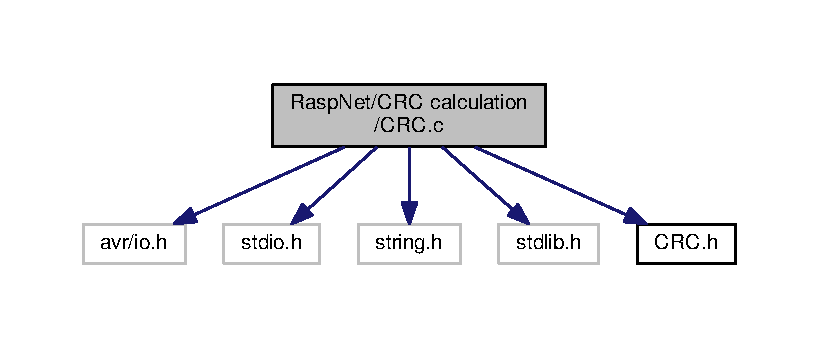
\includegraphics[width=350pt]{CRC_8c__incl}
\end{center}
\end{figure}
This graph shows which files directly or indirectly include this file\+:
\nopagebreak
\begin{figure}[H]
\begin{center}
\leavevmode
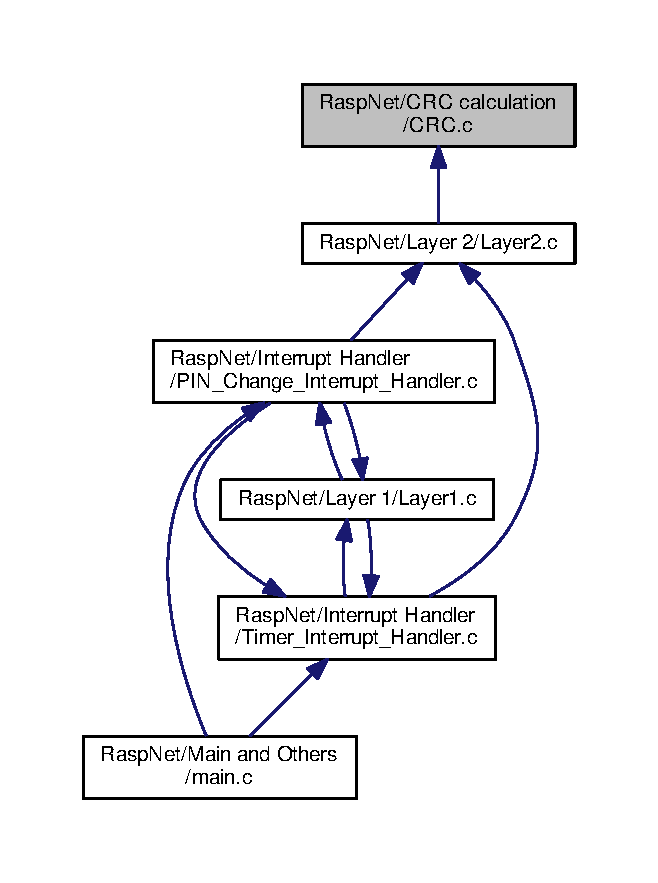
\includegraphics[width=316pt]{CRC_8c__dep__incl}
\end{center}
\end{figure}
\subsection*{Functions}
\begin{DoxyCompactItemize}
\item 
uint32\+\_\+t \hyperlink{CRC_8c_a80a6d5b0482ae9760e75c021a70a4ce1}{C\+R\+C\+\_\+\+Computation} (uint8\+\_\+t $\ast$bytes, int len)
\end{DoxyCompactItemize}


\subsection{Function Documentation}
\index{C\+R\+C.\+c@{C\+R\+C.\+c}!C\+R\+C\+\_\+\+Computation@{C\+R\+C\+\_\+\+Computation}}
\index{C\+R\+C\+\_\+\+Computation@{C\+R\+C\+\_\+\+Computation}!C\+R\+C.\+c@{C\+R\+C.\+c}}
\subsubsection[{\texorpdfstring{C\+R\+C\+\_\+\+Computation(uint8\+\_\+t $\ast$bytes, int len)}{CRC_Computation(uint8_t *bytes, int len)}}]{\setlength{\rightskip}{0pt plus 5cm}uint32\+\_\+t C\+R\+C\+\_\+\+Computation (
\begin{DoxyParamCaption}
\item[{uint8\+\_\+t $\ast$}]{bytes, }
\item[{int}]{len}
\end{DoxyParamCaption}
)}\hypertarget{CRC_8c_a80a6d5b0482ae9760e75c021a70a4ce1}{}\label{CRC_8c_a80a6d5b0482ae9760e75c021a70a4ce1}
$<$ C\+RC polynomial

$<$ Move byte into M\+SB

$<$ Check if M\+SB is 1 or 0

$<$ Left shift 1 and do X\+OR operation

$<$ Left shift 1 if M\+SB is 0 
\begin{DoxyCode}
8                                                 \{
9     \textcolor{keyword}{const} uint64\_t polynomial=0x104C11DB7; 
10     uint32\_t crc = 0;
11     \textcolor{keywordtype}{int} i,byte;
12     \textcolor{keywordflow}{for}(byte=0;byte<len;byte++)\{
13         crc^=((uint32\_t)bytes[byte])<<24; 
14         \textcolor{keywordflow}{for}(i=0;i<8;i++)\{
15             \textcolor{keywordflow}{if}((crc&0x80000000)!=0)\{ 
16                 crc=(uint32\_t)((crc<<1)^polynomial); 
17             \}
18             \textcolor{keywordflow}{else}\{
19                 crc <<= 1; 
21             \}
22         \}
23     \}
24 
25     \textcolor{keywordflow}{return} crc;
26 \}
\end{DoxyCode}

\hypertarget{CRC_8h}{}\section{Rasp\+Net/\+C\+RC calculation/\+C\+RC.h File Reference}
\label{CRC_8h}\index{Rasp\+Net/\+C\+R\+C calculation/\+C\+R\+C.\+h@{Rasp\+Net/\+C\+R\+C calculation/\+C\+R\+C.\+h}}
This graph shows which files directly or indirectly include this file\+:
\nopagebreak
\begin{figure}[H]
\begin{center}
\leavevmode
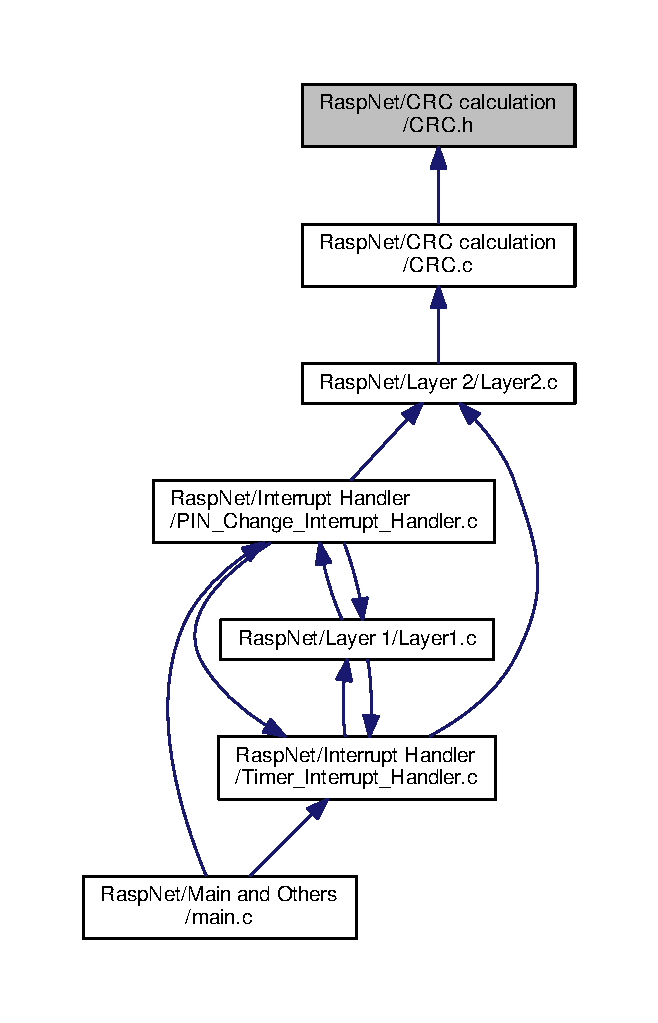
\includegraphics[width=316pt]{CRC_8h__dep__incl}
\end{center}
\end{figure}
\subsection*{Functions}
\begin{DoxyCompactItemize}
\item 
uint32\+\_\+t \hyperlink{CRC_8h_a8ae7190dc3124a566c989b67d5aad3df}{Compute\+\_\+\+C\+R\+C32} (uint8\+\_\+t $\ast$bytes, int len)
\begin{DoxyCompactList}\small\item\em Cyclic Redundancy Check or C\+RC is used to detect error in data. \end{DoxyCompactList}\end{DoxyCompactItemize}


\subsection{Function Documentation}
\index{C\+R\+C.\+h@{C\+R\+C.\+h}!Compute\+\_\+\+C\+R\+C32@{Compute\+\_\+\+C\+R\+C32}}
\index{Compute\+\_\+\+C\+R\+C32@{Compute\+\_\+\+C\+R\+C32}!C\+R\+C.\+h@{C\+R\+C.\+h}}
\subsubsection[{\texorpdfstring{Compute\+\_\+\+C\+R\+C32(uint8\+\_\+t $\ast$bytes, int len)}{Compute_CRC32(uint8_t *bytes, int len)}}]{\setlength{\rightskip}{0pt plus 5cm}uint32\+\_\+t Compute\+\_\+\+C\+R\+C32 (
\begin{DoxyParamCaption}
\item[{uint8\+\_\+t $\ast$}]{bytes, }
\item[{int}]{len}
\end{DoxyParamCaption}
)}\hypertarget{CRC_8h_a8ae7190dc3124a566c989b67d5aad3df}{}\label{CRC_8h_a8ae7190dc3124a566c989b67d5aad3df}


Cyclic Redundancy Check or C\+RC is used to detect error in data. 


\begin{DoxyParams}{Parameters}
{\em bytes} & Integer array which contains payload \\
\hline
{\em len} & of the payload \\
\hline
\end{DoxyParams}
\begin{DoxyReturn}{Returns}
unsigned 32 bit integer is returned which is the computed C\+RC 
\end{DoxyReturn}

\hypertarget{PIN__Change__Interrupt__Handler_8c}{}\section{Rasp\+Net/\+Interrupt Handler/\+P\+I\+N\+\_\+\+Change\+\_\+\+Interrupt\+\_\+\+Handler.c File Reference}
\label{PIN__Change__Interrupt__Handler_8c}\index{Rasp\+Net/\+Interrupt Handler/\+P\+I\+N\+\_\+\+Change\+\_\+\+Interrupt\+\_\+\+Handler.\+c@{Rasp\+Net/\+Interrupt Handler/\+P\+I\+N\+\_\+\+Change\+\_\+\+Interrupt\+\_\+\+Handler.\+c}}
{\ttfamily \#include $<$avr/io.\+h$>$}\\*
{\ttfamily \#include $<$avr/interrupt.\+h$>$}\\*
{\ttfamily \#include \char`\"{}Layer1.\+c\char`\"{}}\\*
{\ttfamily \#include \char`\"{}Layer2.\+c\char`\"{}}\\*
{\ttfamily \#include \char`\"{}Layer3.\+c\char`\"{}}\\*
{\ttfamily \#include \char`\"{}Buffer.\+c\char`\"{}}\\*
{\ttfamily \#include \char`\"{}U\+A\+R\+T\+\_\+\+Handler.\+c\char`\"{}}\\*
{\ttfamily \#include \char`\"{}Timer\+\_\+\+Interrupt\+\_\+\+Handler.\+c\char`\"{}}\\*
{\ttfamily \#include \char`\"{}Miscellaneous.\+c\char`\"{}}\\*
Include dependency graph for P\+I\+N\+\_\+\+Change\+\_\+\+Interrupt\+\_\+\+Handler.\+c\+:
\nopagebreak
\begin{figure}[H]
\begin{center}
\leavevmode
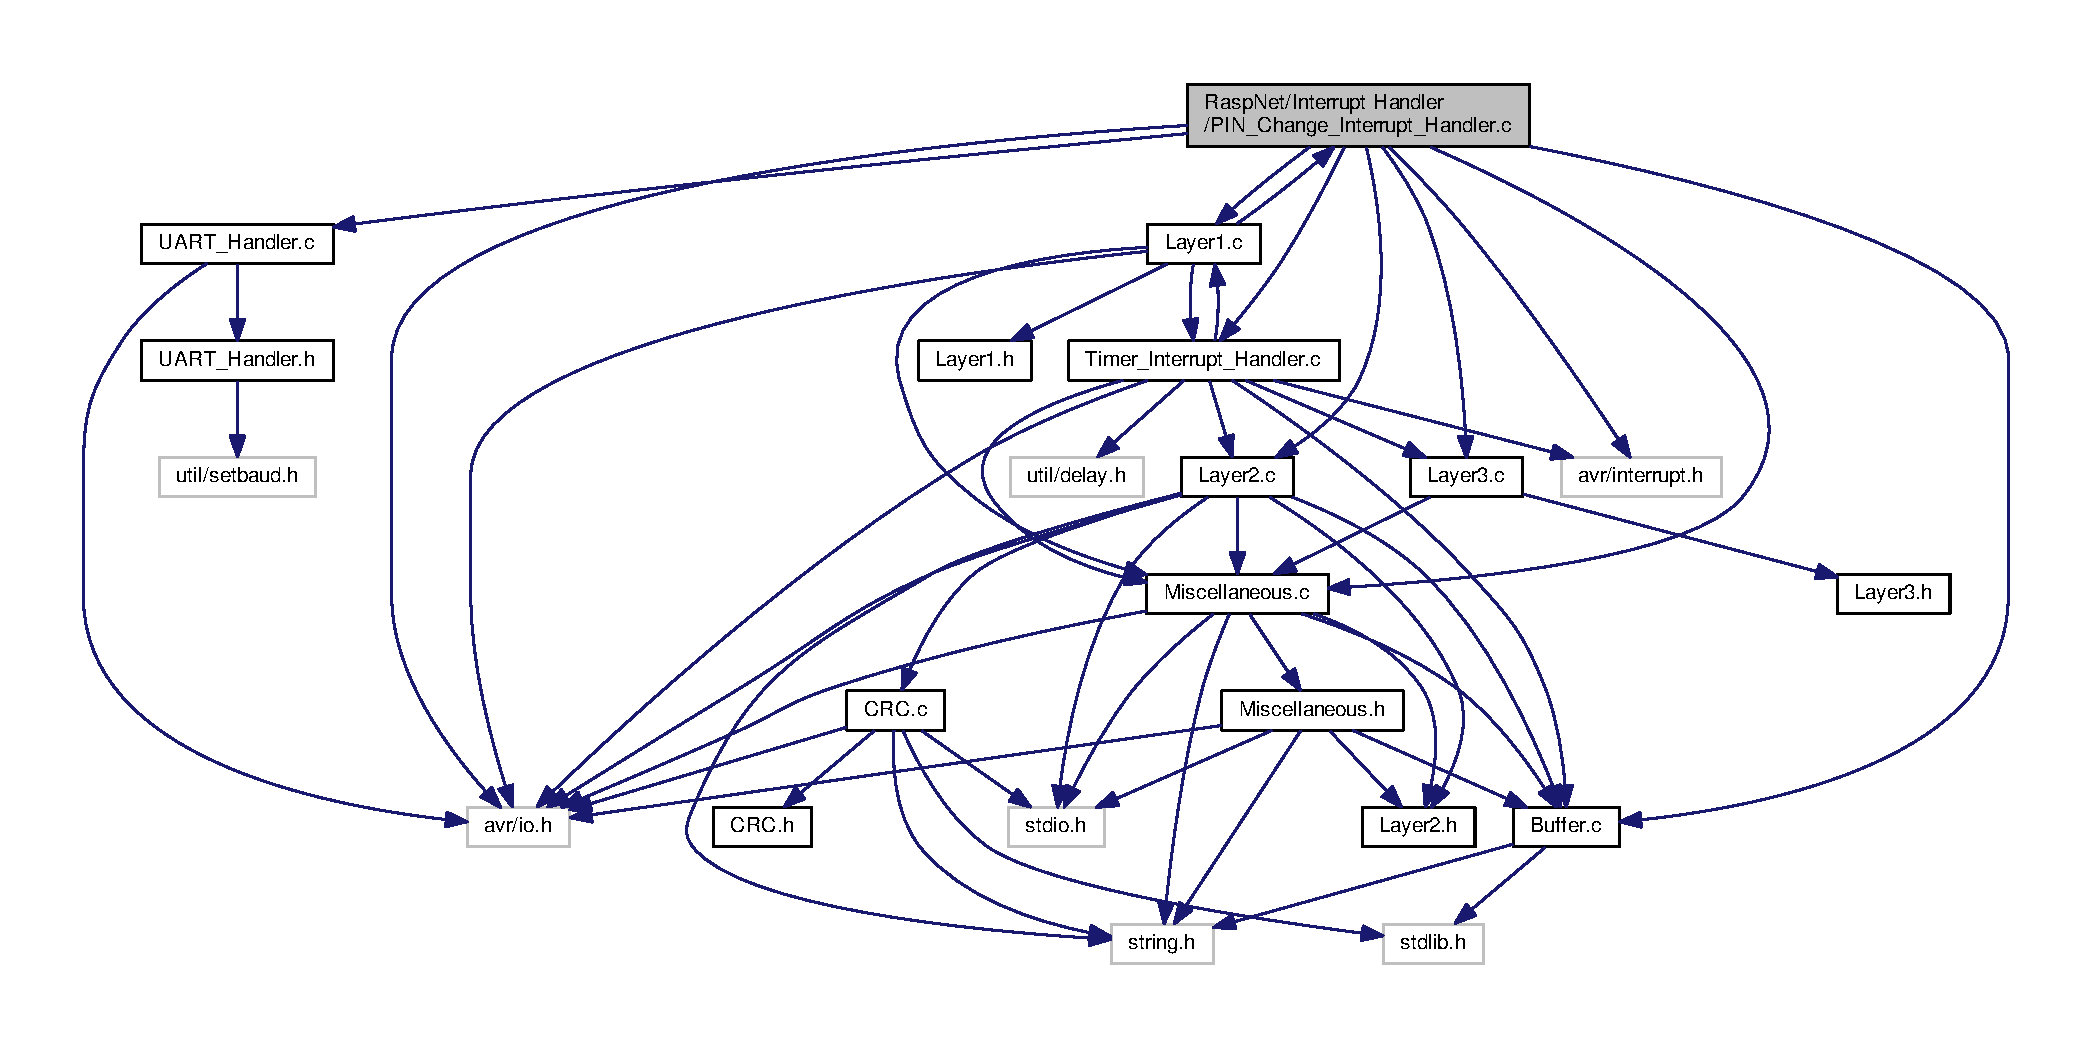
\includegraphics[width=350pt]{PIN__Change__Interrupt__Handler_8c__incl}
\end{center}
\end{figure}
This graph shows which files directly or indirectly include this file\+:
\nopagebreak
\begin{figure}[H]
\begin{center}
\leavevmode
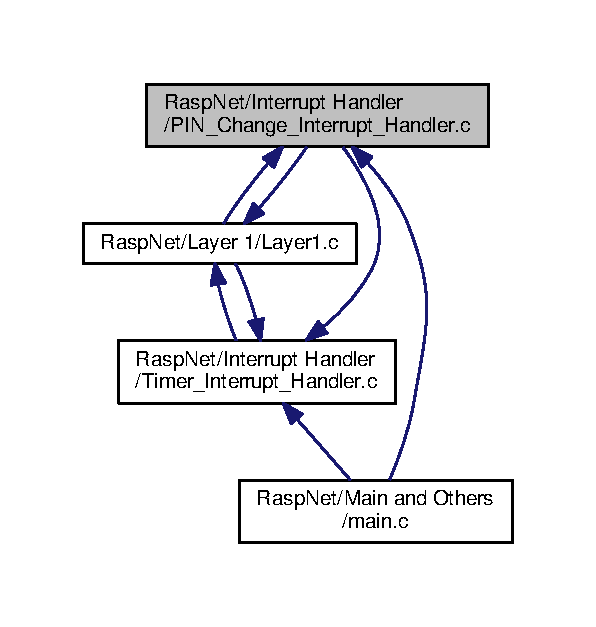
\includegraphics[width=286pt]{PIN__Change__Interrupt__Handler_8c__dep__incl}
\end{center}
\end{figure}
\subsection*{Functions}
\begin{DoxyCompactItemize}
\item 
void \hyperlink{PIN__Change__Interrupt__Handler_8c_acdf613f8022f5390f71cfeb1e84885c7}{pin\+\_\+change\+\_\+interrupt\+\_\+initialization} ()
\item 
\hyperlink{PIN__Change__Interrupt__Handler_8c_a9c4665742c6b6eb1f0bb9dde41f7cba3}{I\+SR} (P\+C\+I\+N\+T2\+\_\+vect)
\end{DoxyCompactItemize}
\subsection*{Variables}
\begin{DoxyCompactItemize}
\item 
int \hyperlink{PIN__Change__Interrupt__Handler_8c_aeae841bbc913f2cc27fe80376dae649f}{Receiver\+Index} =0
\item 
int \hyperlink{PIN__Change__Interrupt__Handler_8c_af6cabaa2e9aa161ceb2c0b36afee5a03}{Receive\+Buffer\+Index} =0
\item 
int \hyperlink{PIN__Change__Interrupt__Handler_8c_a7931d58a3bd94b4566da60f28597d922}{receiver\+\_\+flag} =1
\item 
int \hyperlink{PIN__Change__Interrupt__Handler_8c_a84100ed1f53f510ef91a3d88f24b4b53}{sender\+\_\+flag}
\end{DoxyCompactItemize}


\subsection{Function Documentation}
\index{P\+I\+N\+\_\+\+Change\+\_\+\+Interrupt\+\_\+\+Handler.\+c@{P\+I\+N\+\_\+\+Change\+\_\+\+Interrupt\+\_\+\+Handler.\+c}!I\+SR@{I\+SR}}
\index{I\+SR@{I\+SR}!P\+I\+N\+\_\+\+Change\+\_\+\+Interrupt\+\_\+\+Handler.\+c@{P\+I\+N\+\_\+\+Change\+\_\+\+Interrupt\+\_\+\+Handler.\+c}}
\subsubsection[{\texorpdfstring{I\+S\+R(\+P\+C\+I\+N\+T2\+\_\+vect)}{ISR(PCINT2_vect)}}]{\setlength{\rightskip}{0pt plus 5cm}I\+SR (
\begin{DoxyParamCaption}
\item[{P\+C\+I\+N\+T2\+\_\+vect}]{}
\end{DoxyParamCaption}
)}\hypertarget{PIN__Change__Interrupt__Handler_8c_a9c4665742c6b6eb1f0bb9dde41f7cba3}{}\label{PIN__Change__Interrupt__Handler_8c_a9c4665742c6b6eb1f0bb9dde41f7cba3}
$<$1. Receive preamble which is 8 bit

$<$ Wait until detect the correct preamble

$<$ Receive bit by bit and check

$<$ C\+RC is correct

$<$ Check type of message

$<$1. When message is sent to me

$<$Delete message

$<$ Consider as higher priority

$<$ Received data is put into transmit buffer

$<$Priority is set for R\+E\+L\+AY

$<$ Consider as higher priority

$<$Priority is set for R\+E\+L\+AY

$<$ Start to receive again 
\begin{DoxyCode}
26                  \{
28     \textcolor{keywordflow}{if}(\hyperlink{PIN__Change__Interrupt__Handler_8c_a7931d58a3bd94b4566da60f28597d922}{receiver\_flag}==\hyperlink{Layer3_8h_aa8ef63ae0468c77b8312b92d7154609d}{receive\_preamble}) \{
29         \textcolor{keywordflow}{if}(\hyperlink{Layer2_8c_a5c4475bf56e57eeadef01672aa670a82}{data\_receive}()) \{
30             \hyperlink{Buffer_8c_a60b199d535890694c3b1f82494e64e6d}{receive\_packet\_pointer}->\hyperlink{structPacket_aa305c88136c91911a5159610863cb41d}{preamble}=
      \hyperlink{Miscellaneous_8c_af81f6965e50b219ff38ea272019bac1f}{write\_8\_bit}(\hyperlink{Buffer_8c_a60b199d535890694c3b1f82494e64e6d}{receive\_packet\_pointer}->\hyperlink{structPacket_aa305c88136c91911a5159610863cb41d}{preamble},7-
      \hyperlink{PIN__Change__Interrupt__Handler_8c_aeae841bbc913f2cc27fe80376dae649f}{ReceiverIndex},1);
31             \textcolor{comment}{//uart\_transmission('1');}
32         \}
33         \textcolor{keywordflow}{else} \{
34             \hyperlink{Buffer_8c_a60b199d535890694c3b1f82494e64e6d}{receive\_packet\_pointer}->\hyperlink{structPacket_aa305c88136c91911a5159610863cb41d}{preamble}=
      \hyperlink{Miscellaneous_8c_af81f6965e50b219ff38ea272019bac1f}{write\_8\_bit}(\hyperlink{Buffer_8c_a60b199d535890694c3b1f82494e64e6d}{receive\_packet\_pointer}->\hyperlink{structPacket_aa305c88136c91911a5159610863cb41d}{preamble},7-
      \hyperlink{PIN__Change__Interrupt__Handler_8c_aeae841bbc913f2cc27fe80376dae649f}{ReceiverIndex},0);
35             \textcolor{comment}{//uart\_transmission('0');}
36         \}
37 
38         \hyperlink{PIN__Change__Interrupt__Handler_8c_aeae841bbc913f2cc27fe80376dae649f}{ReceiverIndex}++;
39         \textcolor{keywordflow}{if}(\hyperlink{PIN__Change__Interrupt__Handler_8c_aeae841bbc913f2cc27fe80376dae649f}{ReceiverIndex}>=8) \{
40             \hyperlink{Miscellaneous_8c_afac087d6e168f5fc2cd8994eb07eadb2}{showLog}(\textcolor{stringliteral}{"Received Preamble: "});
41             \hyperlink{Miscellaneous_8c_ae61d07597b559d7305b272b31507f138}{show\_8\_bit\_data}(\hyperlink{Buffer_8c_a60b199d535890694c3b1f82494e64e6d}{receive\_packet\_pointer}->
      \hyperlink{structPacket_aa305c88136c91911a5159610863cb41d}{preamble});
42             \textcolor{keywordflow}{if}(\hyperlink{Miscellaneous_8c_ad063f3ce115eb187d5cbb6fd2b00c0e6}{compare\_preamble}(\hyperlink{Buffer_8c_a60b199d535890694c3b1f82494e64e6d}{receive\_packet\_pointer}->
      \hyperlink{structPacket_aa305c88136c91911a5159610863cb41d}{preamble},\hyperlink{Buffer_8c_ad32f9b2a3c3f3aba80f847dd8c18f77c}{predefined\_preamble})) \{
43                 \hyperlink{Miscellaneous_8c_afac087d6e168f5fc2cd8994eb07eadb2}{showLog}(\textcolor{stringliteral}{"\(\backslash\)nCorrect Preamble\(\backslash\)n"});
44                 \hyperlink{PIN__Change__Interrupt__Handler_8c_aeae841bbc913f2cc27fe80376dae649f}{ReceiverIndex}=0;
45                 \hyperlink{PIN__Change__Interrupt__Handler_8c_a7931d58a3bd94b4566da60f28597d922}{receiver\_flag}=\hyperlink{Layer3_8h_aa59256b98f189dbcee223214dfde1c49}{receive\_crc};
46 
47             \}
48             \textcolor{keywordflow}{else} \{
49                 \textcolor{comment}{//showLog("Wrong preamble\(\backslash\)n");}
51 \textcolor{comment}{}                \hyperlink{Buffer_8c_a60b199d535890694c3b1f82494e64e6d}{receive\_packet\_pointer}->\hyperlink{structPacket_aa305c88136c91911a5159610863cb41d}{preamble}=
      \hyperlink{Buffer_8c_a60b199d535890694c3b1f82494e64e6d}{receive\_packet\_pointer}->\hyperlink{structPacket_aa305c88136c91911a5159610863cb41d}{preamble}<<1;
55             \}
56 
57 
58 
59         \}
60 
61     \}
62 
64     \textcolor{keywordflow}{else} \textcolor{keywordflow}{if}(\hyperlink{PIN__Change__Interrupt__Handler_8c_a7931d58a3bd94b4566da60f28597d922}{receiver\_flag}==\hyperlink{Layer3_8h_aa59256b98f189dbcee223214dfde1c49}{receive\_crc}) \{
65         \textcolor{keywordflow}{if}(\hyperlink{Layer2_8c_a5c4475bf56e57eeadef01672aa670a82}{data\_receive}()) \{
66             \hyperlink{Buffer_8c_a60b199d535890694c3b1f82494e64e6d}{receive\_packet\_pointer}->\hyperlink{structPacket_abad95795e9615463d9d69d298a86b0b8}{crc}=\hyperlink{Miscellaneous_8c_a864fd2a5d36c61fdc91090a497784b55}{write\_32\_bit}(
      \hyperlink{Buffer_8c_a60b199d535890694c3b1f82494e64e6d}{receive\_packet\_pointer}->\hyperlink{structPacket_abad95795e9615463d9d69d298a86b0b8}{crc},31-\hyperlink{PIN__Change__Interrupt__Handler_8c_aeae841bbc913f2cc27fe80376dae649f}{ReceiverIndex},1);
67         \}
68         \textcolor{keywordflow}{else} \{
69             \hyperlink{Buffer_8c_a60b199d535890694c3b1f82494e64e6d}{receive\_packet\_pointer}->\hyperlink{structPacket_abad95795e9615463d9d69d298a86b0b8}{crc}=\hyperlink{Miscellaneous_8c_a864fd2a5d36c61fdc91090a497784b55}{write\_32\_bit}(
      \hyperlink{Buffer_8c_a60b199d535890694c3b1f82494e64e6d}{receive\_packet\_pointer}->\hyperlink{structPacket_abad95795e9615463d9d69d298a86b0b8}{crc},31-\hyperlink{PIN__Change__Interrupt__Handler_8c_aeae841bbc913f2cc27fe80376dae649f}{ReceiverIndex},0);
70         \}
71 
72         \hyperlink{PIN__Change__Interrupt__Handler_8c_aeae841bbc913f2cc27fe80376dae649f}{ReceiverIndex}++;
73         \textcolor{keywordflow}{if}(\hyperlink{PIN__Change__Interrupt__Handler_8c_aeae841bbc913f2cc27fe80376dae649f}{ReceiverIndex}>=32) \{
74             \hyperlink{Miscellaneous_8c_afac087d6e168f5fc2cd8994eb07eadb2}{showLog}(\textcolor{stringliteral}{"Received CRC: "});
75             \hyperlink{Miscellaneous_8c_a4da719f1865290663e587ffb1b00744d}{show\_32\_bit\_data}(\hyperlink{Buffer_8c_a60b199d535890694c3b1f82494e64e6d}{receive\_packet\_pointer}->
      \hyperlink{structPacket_abad95795e9615463d9d69d298a86b0b8}{crc});
76             \hyperlink{PIN__Change__Interrupt__Handler_8c_a7931d58a3bd94b4566da60f28597d922}{receiver\_flag}=\hyperlink{Layer3_8h_a1c9fabd7b0478766bb4b611e5dbe8853}{receive\_payload\_size};
77             \hyperlink{PIN__Change__Interrupt__Handler_8c_aeae841bbc913f2cc27fe80376dae649f}{ReceiverIndex}=0;
78         \}
79 
80     \}
81 
83     \textcolor{keywordflow}{else} \textcolor{keywordflow}{if}(\hyperlink{PIN__Change__Interrupt__Handler_8c_a7931d58a3bd94b4566da60f28597d922}{receiver\_flag}==\hyperlink{Layer3_8h_a1c9fabd7b0478766bb4b611e5dbe8853}{receive\_payload\_size}) \{
84         \textcolor{keywordflow}{if}(\hyperlink{Layer2_8c_a5c4475bf56e57eeadef01672aa670a82}{data\_receive}()) \{
85             \hyperlink{Buffer_8c_a60b199d535890694c3b1f82494e64e6d}{receive\_packet\_pointer}->\hyperlink{structPacket_ab13014675ea9eda122b1c50842a567fc}{payload\_siz}=
      \hyperlink{Miscellaneous_8c_af81f6965e50b219ff38ea272019bac1f}{write\_8\_bit}(\hyperlink{Buffer_8c_a60b199d535890694c3b1f82494e64e6d}{receive\_packet\_pointer}->\hyperlink{structPacket_ab13014675ea9eda122b1c50842a567fc}{payload\_siz},7-
      \hyperlink{PIN__Change__Interrupt__Handler_8c_aeae841bbc913f2cc27fe80376dae649f}{ReceiverIndex},1);
86         \}
87         \textcolor{keywordflow}{else} \{
88             \hyperlink{Buffer_8c_a60b199d535890694c3b1f82494e64e6d}{receive\_packet\_pointer}->\hyperlink{structPacket_ab13014675ea9eda122b1c50842a567fc}{payload\_siz}=
      \hyperlink{Miscellaneous_8c_af81f6965e50b219ff38ea272019bac1f}{write\_8\_bit}(\hyperlink{Buffer_8c_a60b199d535890694c3b1f82494e64e6d}{receive\_packet\_pointer}->\hyperlink{structPacket_ab13014675ea9eda122b1c50842a567fc}{payload\_siz},7-
      \hyperlink{PIN__Change__Interrupt__Handler_8c_aeae841bbc913f2cc27fe80376dae649f}{ReceiverIndex},0);
89         \}
90         \hyperlink{PIN__Change__Interrupt__Handler_8c_aeae841bbc913f2cc27fe80376dae649f}{ReceiverIndex}++;
91         \textcolor{keywordflow}{if}(\hyperlink{PIN__Change__Interrupt__Handler_8c_aeae841bbc913f2cc27fe80376dae649f}{ReceiverIndex}>=8) \{
92             \hyperlink{Miscellaneous_8c_afac087d6e168f5fc2cd8994eb07eadb2}{showLog}(\textcolor{stringliteral}{"Received Payload size: "});
93             \hyperlink{Miscellaneous_8c_ae61d07597b559d7305b272b31507f138}{show\_8\_bit\_data}(\hyperlink{Buffer_8c_a60b199d535890694c3b1f82494e64e6d}{receive\_packet\_pointer}->
      \hyperlink{structPacket_ab13014675ea9eda122b1c50842a567fc}{payload\_siz});
94             \hyperlink{PIN__Change__Interrupt__Handler_8c_a7931d58a3bd94b4566da60f28597d922}{receiver\_flag}=\hyperlink{Layer3_8h_a39e1380303eff462d17201a4cd077b31}{receive\_destination\_address};
95             \hyperlink{PIN__Change__Interrupt__Handler_8c_aeae841bbc913f2cc27fe80376dae649f}{ReceiverIndex}=0;
96         \}
97 
98     \}
99 
101     \textcolor{keywordflow}{else} \textcolor{keywordflow}{if}(\hyperlink{PIN__Change__Interrupt__Handler_8c_a7931d58a3bd94b4566da60f28597d922}{receiver\_flag}==\hyperlink{Layer3_8h_a39e1380303eff462d17201a4cd077b31}{receive\_destination\_address}) \{
102         \textcolor{keywordflow}{if}(\hyperlink{Layer2_8c_a5c4475bf56e57eeadef01672aa670a82}{data\_receive}()) \{
103             \hyperlink{Buffer_8c_a60b199d535890694c3b1f82494e64e6d}{receive\_packet\_pointer}->\hyperlink{structPacket_af626fe07d93fe4116d613304792df080}{destination}=
      \hyperlink{Miscellaneous_8c_af81f6965e50b219ff38ea272019bac1f}{write\_8\_bit}(\hyperlink{Buffer_8c_a60b199d535890694c3b1f82494e64e6d}{receive\_packet\_pointer}->\hyperlink{structPacket_af626fe07d93fe4116d613304792df080}{destination},7-
      \hyperlink{PIN__Change__Interrupt__Handler_8c_aeae841bbc913f2cc27fe80376dae649f}{ReceiverIndex},1);
104 
105         \}
106         \textcolor{keywordflow}{else} \{
107 
108             \hyperlink{Buffer_8c_a60b199d535890694c3b1f82494e64e6d}{receive\_packet\_pointer}->\hyperlink{structPacket_af626fe07d93fe4116d613304792df080}{destination}=
      \hyperlink{Miscellaneous_8c_af81f6965e50b219ff38ea272019bac1f}{write\_8\_bit}(\hyperlink{Buffer_8c_a60b199d535890694c3b1f82494e64e6d}{receive\_packet\_pointer}->\hyperlink{structPacket_af626fe07d93fe4116d613304792df080}{destination},7-
      \hyperlink{PIN__Change__Interrupt__Handler_8c_aeae841bbc913f2cc27fe80376dae649f}{ReceiverIndex},0);
109         \}
110 
111         \hyperlink{PIN__Change__Interrupt__Handler_8c_aeae841bbc913f2cc27fe80376dae649f}{ReceiverIndex}++;
112         \textcolor{keywordflow}{if}(\hyperlink{PIN__Change__Interrupt__Handler_8c_aeae841bbc913f2cc27fe80376dae649f}{ReceiverIndex}>=8) \{
113             \hyperlink{Buffer_8c_a60b199d535890694c3b1f82494e64e6d}{receive\_packet\_pointer}->\hyperlink{structPacket_a58a48ac639979f488f254bbcb98e72b8}{payload}[0]=
      \hyperlink{Buffer_8c_a60b199d535890694c3b1f82494e64e6d}{receive\_packet\_pointer}->\hyperlink{structPacket_af626fe07d93fe4116d613304792df080}{destination};
114             \hyperlink{Miscellaneous_8c_afac087d6e168f5fc2cd8994eb07eadb2}{showLog}(\textcolor{stringliteral}{"\(\backslash\)nReceived Destination address\(\backslash\)n"});
115             \hyperlink{Miscellaneous_8c_ae61d07597b559d7305b272b31507f138}{show\_8\_bit\_data}(\hyperlink{Buffer_8c_a60b199d535890694c3b1f82494e64e6d}{receive\_packet\_pointer}->
      \hyperlink{structPacket_af626fe07d93fe4116d613304792df080}{destination});
116             \hyperlink{PIN__Change__Interrupt__Handler_8c_a7931d58a3bd94b4566da60f28597d922}{receiver\_flag}=\hyperlink{Layer3_8h_ace2bdbcd80ee617b80126b378b51dfe3}{receive\_source\_address};
117             \hyperlink{PIN__Change__Interrupt__Handler_8c_aeae841bbc913f2cc27fe80376dae649f}{ReceiverIndex}=0;
118         \}
119 
120     \}
121 
123     \textcolor{keywordflow}{else} \textcolor{keywordflow}{if}(\hyperlink{PIN__Change__Interrupt__Handler_8c_a7931d58a3bd94b4566da60f28597d922}{receiver\_flag}==\hyperlink{Layer3_8h_ace2bdbcd80ee617b80126b378b51dfe3}{receive\_source\_address}) \{
124         \textcolor{keywordflow}{if}(\hyperlink{Layer2_8c_a5c4475bf56e57eeadef01672aa670a82}{data\_receive}()) \{
125             \hyperlink{Buffer_8c_a60b199d535890694c3b1f82494e64e6d}{receive\_packet\_pointer}->\hyperlink{structPacket_a01308f5b690e5060fea6037e765058b9}{source}=
      \hyperlink{Miscellaneous_8c_af81f6965e50b219ff38ea272019bac1f}{write\_8\_bit}(\hyperlink{Buffer_8c_a60b199d535890694c3b1f82494e64e6d}{receive\_packet\_pointer}->\hyperlink{structPacket_a01308f5b690e5060fea6037e765058b9}{source},7-
      \hyperlink{PIN__Change__Interrupt__Handler_8c_aeae841bbc913f2cc27fe80376dae649f}{ReceiverIndex},1);
126         \}
127         \textcolor{keywordflow}{else} \{
128             \hyperlink{Buffer_8c_a60b199d535890694c3b1f82494e64e6d}{receive\_packet\_pointer}->\hyperlink{structPacket_a01308f5b690e5060fea6037e765058b9}{source}=
      \hyperlink{Miscellaneous_8c_af81f6965e50b219ff38ea272019bac1f}{write\_8\_bit}(\hyperlink{Buffer_8c_a60b199d535890694c3b1f82494e64e6d}{receive\_packet\_pointer}->\hyperlink{structPacket_a01308f5b690e5060fea6037e765058b9}{source},7-
      \hyperlink{PIN__Change__Interrupt__Handler_8c_aeae841bbc913f2cc27fe80376dae649f}{ReceiverIndex},0);
129         \}
130         \hyperlink{PIN__Change__Interrupt__Handler_8c_aeae841bbc913f2cc27fe80376dae649f}{ReceiverIndex}++;
131         \textcolor{keywordflow}{if}(\hyperlink{PIN__Change__Interrupt__Handler_8c_aeae841bbc913f2cc27fe80376dae649f}{ReceiverIndex}>=8) \{
132             \hyperlink{Buffer_8c_a60b199d535890694c3b1f82494e64e6d}{receive\_packet\_pointer}->\hyperlink{structPacket_a58a48ac639979f488f254bbcb98e72b8}{payload}[1]=
      \hyperlink{Buffer_8c_a60b199d535890694c3b1f82494e64e6d}{receive\_packet\_pointer}->\hyperlink{structPacket_a01308f5b690e5060fea6037e765058b9}{source};
133             \hyperlink{Miscellaneous_8c_afac087d6e168f5fc2cd8994eb07eadb2}{showLog}(\textcolor{stringliteral}{"\(\backslash\)nReceived source address\(\backslash\)n"});
134             \hyperlink{PIN__Change__Interrupt__Handler_8c_a7931d58a3bd94b4566da60f28597d922}{receiver\_flag}=\hyperlink{Layer3_8h_a8fc3575b730c4bc458cdce87537175d1}{receive\_payload};
135             \hyperlink{Miscellaneous_8c_ae61d07597b559d7305b272b31507f138}{show\_8\_bit\_data}(\hyperlink{Buffer_8c_a60b199d535890694c3b1f82494e64e6d}{receive\_packet\_pointer}->
      \hyperlink{structPacket_a01308f5b690e5060fea6037e765058b9}{source});
136             \hyperlink{PIN__Change__Interrupt__Handler_8c_aeae841bbc913f2cc27fe80376dae649f}{ReceiverIndex}=0;
137             \hyperlink{PIN__Change__Interrupt__Handler_8c_af6cabaa2e9aa161ceb2c0b36afee5a03}{ReceiveBufferIndex}=2;
138         \}
139 
140     \}
141 
143     \textcolor{keywordflow}{else} \textcolor{keywordflow}{if}(\hyperlink{PIN__Change__Interrupt__Handler_8c_a7931d58a3bd94b4566da60f28597d922}{receiver\_flag}==\hyperlink{Layer3_8h_a8fc3575b730c4bc458cdce87537175d1}{receive\_payload}) \{
144         \textcolor{keywordflow}{if}(\hyperlink{Layer2_8c_a5c4475bf56e57eeadef01672aa670a82}{data\_receive}()) \{
145             \hyperlink{Buffer_8c_a60b199d535890694c3b1f82494e64e6d}{receive\_packet\_pointer}->\hyperlink{structPacket_a58a48ac639979f488f254bbcb98e72b8}{payload}[
      \hyperlink{PIN__Change__Interrupt__Handler_8c_af6cabaa2e9aa161ceb2c0b36afee5a03}{ReceiveBufferIndex}]=\hyperlink{Miscellaneous_8c_af81f6965e50b219ff38ea272019bac1f}{write\_8\_bit}(
      \hyperlink{Buffer_8c_a60b199d535890694c3b1f82494e64e6d}{receive\_packet\_pointer}->\hyperlink{structPacket_a58a48ac639979f488f254bbcb98e72b8}{payload}[\hyperlink{PIN__Change__Interrupt__Handler_8c_af6cabaa2e9aa161ceb2c0b36afee5a03}{ReceiveBufferIndex}],(7-(
      \hyperlink{PIN__Change__Interrupt__Handler_8c_aeae841bbc913f2cc27fe80376dae649f}{ReceiverIndex}%8)),1);
146         \}
147         \textcolor{keywordflow}{else} \{
148             \hyperlink{Buffer_8c_a60b199d535890694c3b1f82494e64e6d}{receive\_packet\_pointer}->\hyperlink{structPacket_a58a48ac639979f488f254bbcb98e72b8}{payload}[
      \hyperlink{PIN__Change__Interrupt__Handler_8c_af6cabaa2e9aa161ceb2c0b36afee5a03}{ReceiveBufferIndex}]=\hyperlink{Miscellaneous_8c_af81f6965e50b219ff38ea272019bac1f}{write\_8\_bit}(
      \hyperlink{Buffer_8c_a60b199d535890694c3b1f82494e64e6d}{receive\_packet\_pointer}->\hyperlink{structPacket_a58a48ac639979f488f254bbcb98e72b8}{payload}[\hyperlink{PIN__Change__Interrupt__Handler_8c_af6cabaa2e9aa161ceb2c0b36afee5a03}{ReceiveBufferIndex}],(7-(
      \hyperlink{PIN__Change__Interrupt__Handler_8c_aeae841bbc913f2cc27fe80376dae649f}{ReceiverIndex}%8)),0);
149         \}
150 
151         \hyperlink{PIN__Change__Interrupt__Handler_8c_aeae841bbc913f2cc27fe80376dae649f}{ReceiverIndex}++;
152         \textcolor{keywordflow}{if}(\hyperlink{PIN__Change__Interrupt__Handler_8c_aeae841bbc913f2cc27fe80376dae649f}{ReceiverIndex}%8==0) \{
153             \hyperlink{PIN__Change__Interrupt__Handler_8c_af6cabaa2e9aa161ceb2c0b36afee5a03}{ReceiveBufferIndex}=\hyperlink{PIN__Change__Interrupt__Handler_8c_af6cabaa2e9aa161ceb2c0b36afee5a03}{ReceiveBufferIndex}+1;
154         \}
155 
156 
157         \textcolor{keywordflow}{if}(\hyperlink{PIN__Change__Interrupt__Handler_8c_aeae841bbc913f2cc27fe80376dae649f}{ReceiverIndex}>=(((\hyperlink{Buffer_8c_a60b199d535890694c3b1f82494e64e6d}{receive\_packet\_pointer}->
      \hyperlink{structPacket_ab13014675ea9eda122b1c50842a567fc}{payload\_siz})-2)*8)) \{
158             \hyperlink{PIN__Change__Interrupt__Handler_8c_a7931d58a3bd94b4566da60f28597d922}{receiver\_flag}=\hyperlink{Layer3_8h_ae248a94ed37c2d8dad80d8a627ad9974}{received\_crc\_check};
159             \hyperlink{PIN__Change__Interrupt__Handler_8c_aeae841bbc913f2cc27fe80376dae649f}{ReceiverIndex}=0;
160             \hyperlink{Miscellaneous_8c_afac087d6e168f5fc2cd8994eb07eadb2}{showLog}(\textcolor{stringliteral}{"Received payload: "});
161             \hyperlink{Miscellaneous_8c_a9ea1d4b6a27b5caa55c150b2ba17983a}{show\_payload}(\hyperlink{Buffer_8c_a60b199d535890694c3b1f82494e64e6d}{receive\_packet\_pointer}->
      \hyperlink{structPacket_a58a48ac639979f488f254bbcb98e72b8}{payload},\hyperlink{Buffer_8c_a60b199d535890694c3b1f82494e64e6d}{receive\_packet\_pointer}->\hyperlink{structPacket_ab13014675ea9eda122b1c50842a567fc}{payload\_siz});
162 
163         \}
164 
165     \}
166 
168     \textcolor{keywordflow}{else} \textcolor{keywordflow}{if}(\hyperlink{PIN__Change__Interrupt__Handler_8c_a7931d58a3bd94b4566da60f28597d922}{receiver\_flag}==\hyperlink{Layer3_8h_ae248a94ed37c2d8dad80d8a627ad9974}{received\_crc\_check}) \{
169         uint32\_t crc\_calculation=\hyperlink{CRC_8c_a80a6d5b0482ae9760e75c021a70a4ce1}{CRC\_Computation}(
      \hyperlink{Buffer_8c_a60b199d535890694c3b1f82494e64e6d}{receive\_packet\_pointer}->\hyperlink{structPacket_a58a48ac639979f488f254bbcb98e72b8}{payload},
      \hyperlink{Buffer_8c_a60b199d535890694c3b1f82494e64e6d}{receive\_packet\_pointer}->\hyperlink{structPacket_ab13014675ea9eda122b1c50842a567fc}{payload\_siz});
170         \hyperlink{Miscellaneous_8c_afac087d6e168f5fc2cd8994eb07eadb2}{showLog}(\textcolor{stringliteral}{"CRC Check: \(\backslash\)n"});
172         \textcolor{keywordflow}{if}(\hyperlink{Miscellaneous_8c_a7ea454e652a249ba5f17f6233e65887a}{compare\_crc}(crc\_calculation,\hyperlink{Buffer_8c_a60b199d535890694c3b1f82494e64e6d}{receive\_packet\_pointer}->
      \hyperlink{structPacket_abad95795e9615463d9d69d298a86b0b8}{crc})) \{
173             \hyperlink{Miscellaneous_8c_afac087d6e168f5fc2cd8994eb07eadb2}{showLog}(\textcolor{stringliteral}{"Correct CRC"});
174             \textcolor{keywordtype}{int} message\_type=\hyperlink{Layer3_8c_a23b38c7493fb43e33264c3972782f496}{type\_of\_msg}(\hyperlink{Buffer_8c_a60b199d535890694c3b1f82494e64e6d}{receive\_packet\_pointer}); 
177             \textcolor{keywordflow}{if}(message\_type==\hyperlink{Layer3_8h_a465792308892364b6fd0d58cf45b6043}{msg\_send\_to\_me}) \{
178                 \hyperlink{Miscellaneous_8c_afac087d6e168f5fc2cd8994eb07eadb2}{showLog}(\textcolor{stringliteral}{"Message send to me"});
179                 \hyperlink{Layer3_8c_a5cc35a45674625cd8733379d3f0523b8}{discard\_packet}(\hyperlink{Buffer_8c_a60b199d535890694c3b1f82494e64e6d}{receive\_packet\_pointer});
180                 \textcolor{comment}{//transmit\_packet=my\_own\_packet;}
181 
182 
183             \}
184 
186             \textcolor{keywordflow}{else} \textcolor{keywordflow}{if}(message\_type==\hyperlink{Layer3_8h_a8aa9037a9afe926a10f769adc957936a}{msg\_send\_to\_other\_node}) \{
187                 \hyperlink{Layer3_8h_a2a0eb18d69ebbaf44dd4e863fa4f6a59}{priority\_type}=\hyperlink{Layer3_8h_a4a793a607f3e830119fe598d76630898}{priority\_high}; 
188                 \textcolor{keywordflow}{if}(\hyperlink{PIN__Change__Interrupt__Handler_8c_a84100ed1f53f510ef91a3d88f24b4b53}{sender\_flag}==\hyperlink{Layer3_8h_af43b7652801ee9e083162514d5372e9f}{transmitted})\{
189                     \hyperlink{PIN__Change__Interrupt__Handler_8c_a84100ed1f53f510ef91a3d88f24b4b53}{sender\_flag}=\hyperlink{Layer3_8h_a5b4f913d88d52723f970056a0ea4dd09}{transmit\_preamble};
190                 \}
191                 *\hyperlink{Buffer_8c_ac229f7d7f062771563514df9f3927eb6}{transmit\_packet\_pointer}=*
      \hyperlink{Buffer_8c_a60b199d535890694c3b1f82494e64e6d}{receive\_packet\_pointer}; 
192                 \hyperlink{Miscellaneous_8c_afac087d6e168f5fc2cd8994eb07eadb2}{showLog}(\textcolor{stringliteral}{"Message send to other"});
193 
194                 \hyperlink{Layer3_8h_a2a0eb18d69ebbaf44dd4e863fa4f6a59}{priority\_type}=\hyperlink{Layer3_8h_aaccf0a951ca84ac3578fa3bcfbac5522}{priority\_for\_relay}; 
196             \}
197 
199             \textcolor{keywordflow}{else} \textcolor{keywordflow}{if}(message\_type==\hyperlink{Layer3_8h_a3bd3ae1527491d97c67f22e569f296a4}{broadcasting\_msg}) \{
200                 \hyperlink{Layer3_8h_a2a0eb18d69ebbaf44dd4e863fa4f6a59}{priority\_type}=\hyperlink{Layer3_8h_a4a793a607f3e830119fe598d76630898}{priority\_high}; 
201                 \hyperlink{Miscellaneous_8c_afac087d6e168f5fc2cd8994eb07eadb2}{showLog}(\textcolor{stringliteral}{"Broadcasting Message"});
202 
203                 \textcolor{keywordflow}{if}(\hyperlink{PIN__Change__Interrupt__Handler_8c_a84100ed1f53f510ef91a3d88f24b4b53}{sender\_flag}==\hyperlink{Layer3_8h_af43b7652801ee9e083162514d5372e9f}{transmitted})\{
204                         \hyperlink{PIN__Change__Interrupt__Handler_8c_a84100ed1f53f510ef91a3d88f24b4b53}{sender\_flag}=\hyperlink{Layer3_8h_a5b4f913d88d52723f970056a0ea4dd09}{transmit\_preamble};
205                 \}
206                 *\hyperlink{Buffer_8c_ac229f7d7f062771563514df9f3927eb6}{transmit\_packet\_pointer}=*
      \hyperlink{Buffer_8c_a60b199d535890694c3b1f82494e64e6d}{receive\_packet\_pointer};
207                 \hyperlink{Layer3_8h_a2a0eb18d69ebbaf44dd4e863fa4f6a59}{priority\_type}=\hyperlink{Layer3_8h_aaccf0a951ca84ac3578fa3bcfbac5522}{priority\_for\_relay}; 
210             \}
211 
213             \textcolor{keywordflow}{else} \textcolor{keywordflow}{if}(message\_type==\hyperlink{Layer3_8h_ab7153c7289145c9aab31e838d3f29b0f}{return\_my\_own\_msg}) \{
214                 \hyperlink{Miscellaneous_8c_afac087d6e168f5fc2cd8994eb07eadb2}{showLog}(\textcolor{stringliteral}{"Return my own messsage"});
215                 \hyperlink{Miscellaneous_8c_afac087d6e168f5fc2cd8994eb07eadb2}{showLog}(\textcolor{stringliteral}{"Discard packet"});
216                 *\hyperlink{Buffer_8c_ac229f7d7f062771563514df9f3927eb6}{transmit\_packet\_pointer}= *
      \hyperlink{Buffer_8c_ac247c7d61e5a6e7abecd95209dae8bcb}{my\_own\_packet\_pointer};
217                 \hyperlink{Layer3_8c_a5cc35a45674625cd8733379d3f0523b8}{discard\_packet}(\hyperlink{Buffer_8c_a60b199d535890694c3b1f82494e64e6d}{receive\_packet\_pointer});
218                 \hyperlink{PIN__Change__Interrupt__Handler_8c_a84100ed1f53f510ef91a3d88f24b4b53}{sender\_flag}=\hyperlink{Layer3_8h_a5b4f913d88d52723f970056a0ea4dd09}{transmit\_preamble};
219                 \hyperlink{Layer3_8h_a2a0eb18d69ebbaf44dd4e863fa4f6a59}{priority\_type}=\hyperlink{Layer3_8h_a3b7ed14628679beda488dc3269b7b6a0}{priority\_for\_sending\_order};
220 
221             \}
222 
224             \textcolor{keywordflow}{else} \textcolor{keywordflow}{if}(message\_type==\hyperlink{Layer3_8h_a58352e6aa962709f6a002dbc21406113}{my\_own\_braodcasting\_msg}) \{
225                 \hyperlink{Miscellaneous_8c_afac087d6e168f5fc2cd8994eb07eadb2}{showLog}(\textcolor{stringliteral}{"My own broadcasting Messsage"});
226                 \hyperlink{Miscellaneous_8c_afac087d6e168f5fc2cd8994eb07eadb2}{showLog}(\textcolor{stringliteral}{"Discard packet"});
227                 *\hyperlink{Buffer_8c_ac229f7d7f062771563514df9f3927eb6}{transmit\_packet\_pointer}= *
      \hyperlink{Buffer_8c_ac247c7d61e5a6e7abecd95209dae8bcb}{my\_own\_packet\_pointer};
228                 \hyperlink{Layer3_8c_a5cc35a45674625cd8733379d3f0523b8}{discard\_packet}(\hyperlink{Buffer_8c_a60b199d535890694c3b1f82494e64e6d}{receive\_packet\_pointer});
229                 \hyperlink{PIN__Change__Interrupt__Handler_8c_a84100ed1f53f510ef91a3d88f24b4b53}{sender\_flag}=\hyperlink{Layer3_8h_a5b4f913d88d52723f970056a0ea4dd09}{transmit\_preamble};
230                 \hyperlink{Layer3_8h_a2a0eb18d69ebbaf44dd4e863fa4f6a59}{priority\_type}=\hyperlink{Layer3_8h_a3b7ed14628679beda488dc3269b7b6a0}{priority\_for\_sending\_order};
231 
232             \}
234             \textcolor{keywordflow}{else} \textcolor{keywordflow}{if}(message\_type==\hyperlink{Layer3_8h_a09741204cd73a0942c6f97dd0e9d3108}{unknown})\{
235                 \hyperlink{Miscellaneous_8c_afac087d6e168f5fc2cd8994eb07eadb2}{showLog}(\textcolor{stringliteral}{"Unknown Message"});
236             \}
237 
238             \hyperlink{PIN__Change__Interrupt__Handler_8c_a7931d58a3bd94b4566da60f28597d922}{receiver\_flag}=\hyperlink{Layer3_8h_aa8ef63ae0468c77b8312b92d7154609d}{receive\_preamble}; 
239             \textcolor{comment}{//discard\_packet(receive\_packet\_pointer);}
240             \hyperlink{Miscellaneous_8c_afac087d6e168f5fc2cd8994eb07eadb2}{showLog}(\textcolor{stringliteral}{"----------Receive Cycle Finish----------"});
241 
242         \}
243 
245         \textcolor{keywordflow}{else} \{
246             \hyperlink{Miscellaneous_8c_afac087d6e168f5fc2cd8994eb07eadb2}{showLog}(\textcolor{stringliteral}{"Wrong CRC"});
247             \hyperlink{Layer3_8c_a5cc35a45674625cd8733379d3f0523b8}{discard\_packet}(\hyperlink{Buffer_8c_a60b199d535890694c3b1f82494e64e6d}{receive\_packet\_pointer});
248             \hyperlink{PIN__Change__Interrupt__Handler_8c_a7931d58a3bd94b4566da60f28597d922}{receiver\_flag}=\hyperlink{Layer3_8h_aa8ef63ae0468c77b8312b92d7154609d}{receive\_preamble};
249 
250         \}
251 
252         \hyperlink{PIN__Change__Interrupt__Handler_8c_aeae841bbc913f2cc27fe80376dae649f}{ReceiverIndex}=0;
253 
254     \}
255 
256 
257 \}
\end{DoxyCode}
\index{P\+I\+N\+\_\+\+Change\+\_\+\+Interrupt\+\_\+\+Handler.\+c@{P\+I\+N\+\_\+\+Change\+\_\+\+Interrupt\+\_\+\+Handler.\+c}!pin\+\_\+change\+\_\+interrupt\+\_\+initialization@{pin\+\_\+change\+\_\+interrupt\+\_\+initialization}}
\index{pin\+\_\+change\+\_\+interrupt\+\_\+initialization@{pin\+\_\+change\+\_\+interrupt\+\_\+initialization}!P\+I\+N\+\_\+\+Change\+\_\+\+Interrupt\+\_\+\+Handler.\+c@{P\+I\+N\+\_\+\+Change\+\_\+\+Interrupt\+\_\+\+Handler.\+c}}
\subsubsection[{\texorpdfstring{pin\+\_\+change\+\_\+interrupt\+\_\+initialization()}{pin_change_interrupt_initialization()}}]{\setlength{\rightskip}{0pt plus 5cm}void pin\+\_\+change\+\_\+interrupt\+\_\+initialization (
\begin{DoxyParamCaption}
{}
\end{DoxyParamCaption}
)}\hypertarget{PIN__Change__Interrupt__Handler_8c_acdf613f8022f5390f71cfeb1e84885c7}{}\label{PIN__Change__Interrupt__Handler_8c_acdf613f8022f5390f71cfeb1e84885c7}
P\+IN Change interrupt is used for receiving data $<$ enabled P\+C\+I\+NT\mbox{[}23\+:16\mbox{]} pin will cause an interrupt

$<$ pin change interrupt for P\+D4 or clock receive signal 
\begin{DoxyCode}
50                                           \{
51   PCICR|= (1<<PCIE2); 
52   PCMSK2|=(1<<PCINT20);
53 \}
\end{DoxyCode}


\subsection{Variable Documentation}
\index{P\+I\+N\+\_\+\+Change\+\_\+\+Interrupt\+\_\+\+Handler.\+c@{P\+I\+N\+\_\+\+Change\+\_\+\+Interrupt\+\_\+\+Handler.\+c}!Receive\+Buffer\+Index@{Receive\+Buffer\+Index}}
\index{Receive\+Buffer\+Index@{Receive\+Buffer\+Index}!P\+I\+N\+\_\+\+Change\+\_\+\+Interrupt\+\_\+\+Handler.\+c@{P\+I\+N\+\_\+\+Change\+\_\+\+Interrupt\+\_\+\+Handler.\+c}}
\subsubsection[{\texorpdfstring{Receive\+Buffer\+Index}{ReceiveBufferIndex}}]{\setlength{\rightskip}{0pt plus 5cm}int Receive\+Buffer\+Index =0}\hypertarget{PIN__Change__Interrupt__Handler_8c_af6cabaa2e9aa161ceb2c0b36afee5a03}{}\label{PIN__Change__Interrupt__Handler_8c_af6cabaa2e9aa161ceb2c0b36afee5a03}
\index{P\+I\+N\+\_\+\+Change\+\_\+\+Interrupt\+\_\+\+Handler.\+c@{P\+I\+N\+\_\+\+Change\+\_\+\+Interrupt\+\_\+\+Handler.\+c}!receiver\+\_\+flag@{receiver\+\_\+flag}}
\index{receiver\+\_\+flag@{receiver\+\_\+flag}!P\+I\+N\+\_\+\+Change\+\_\+\+Interrupt\+\_\+\+Handler.\+c@{P\+I\+N\+\_\+\+Change\+\_\+\+Interrupt\+\_\+\+Handler.\+c}}
\subsubsection[{\texorpdfstring{receiver\+\_\+flag}{receiver_flag}}]{\setlength{\rightskip}{0pt plus 5cm}int receiver\+\_\+flag =1}\hypertarget{PIN__Change__Interrupt__Handler_8c_a7931d58a3bd94b4566da60f28597d922}{}\label{PIN__Change__Interrupt__Handler_8c_a7931d58a3bd94b4566da60f28597d922}
\index{P\+I\+N\+\_\+\+Change\+\_\+\+Interrupt\+\_\+\+Handler.\+c@{P\+I\+N\+\_\+\+Change\+\_\+\+Interrupt\+\_\+\+Handler.\+c}!Receiver\+Index@{Receiver\+Index}}
\index{Receiver\+Index@{Receiver\+Index}!P\+I\+N\+\_\+\+Change\+\_\+\+Interrupt\+\_\+\+Handler.\+c@{P\+I\+N\+\_\+\+Change\+\_\+\+Interrupt\+\_\+\+Handler.\+c}}
\subsubsection[{\texorpdfstring{Receiver\+Index}{ReceiverIndex}}]{\setlength{\rightskip}{0pt plus 5cm}int Receiver\+Index =0}\hypertarget{PIN__Change__Interrupt__Handler_8c_aeae841bbc913f2cc27fe80376dae649f}{}\label{PIN__Change__Interrupt__Handler_8c_aeae841bbc913f2cc27fe80376dae649f}
\index{P\+I\+N\+\_\+\+Change\+\_\+\+Interrupt\+\_\+\+Handler.\+c@{P\+I\+N\+\_\+\+Change\+\_\+\+Interrupt\+\_\+\+Handler.\+c}!sender\+\_\+flag@{sender\+\_\+flag}}
\index{sender\+\_\+flag@{sender\+\_\+flag}!P\+I\+N\+\_\+\+Change\+\_\+\+Interrupt\+\_\+\+Handler.\+c@{P\+I\+N\+\_\+\+Change\+\_\+\+Interrupt\+\_\+\+Handler.\+c}}
\subsubsection[{\texorpdfstring{sender\+\_\+flag}{sender_flag}}]{\setlength{\rightskip}{0pt plus 5cm}int sender\+\_\+flag}\hypertarget{PIN__Change__Interrupt__Handler_8c_a84100ed1f53f510ef91a3d88f24b4b53}{}\label{PIN__Change__Interrupt__Handler_8c_a84100ed1f53f510ef91a3d88f24b4b53}

\hypertarget{Timer__Interrupt__Handler_8c}{}\section{Rasp\+Net/\+Interrupt Handler/\+Timer\+\_\+\+Interrupt\+\_\+\+Handler.c File Reference}
\label{Timer__Interrupt__Handler_8c}\index{Rasp\+Net/\+Interrupt Handler/\+Timer\+\_\+\+Interrupt\+\_\+\+Handler.\+c@{Rasp\+Net/\+Interrupt Handler/\+Timer\+\_\+\+Interrupt\+\_\+\+Handler.\+c}}
{\ttfamily \#include $<$avr/io.\+h$>$}\\*
{\ttfamily \#include $<$avr/interrupt.\+h$>$}\\*
{\ttfamily \#include $<$util/delay.\+h$>$}\\*
{\ttfamily \#include \char`\"{}Layer1.\+c\char`\"{}}\\*
{\ttfamily \#include \char`\"{}Layer2.\+c\char`\"{}}\\*
{\ttfamily \#include \char`\"{}Layer3.\+c\char`\"{}}\\*
{\ttfamily \#include \char`\"{}Buffer.\+c\char`\"{}}\\*
{\ttfamily \#include \char`\"{}Miscellaneous.\+c\char`\"{}}\\*
Include dependency graph for Timer\+\_\+\+Interrupt\+\_\+\+Handler.\+c\+:
\nopagebreak
\begin{figure}[H]
\begin{center}
\leavevmode
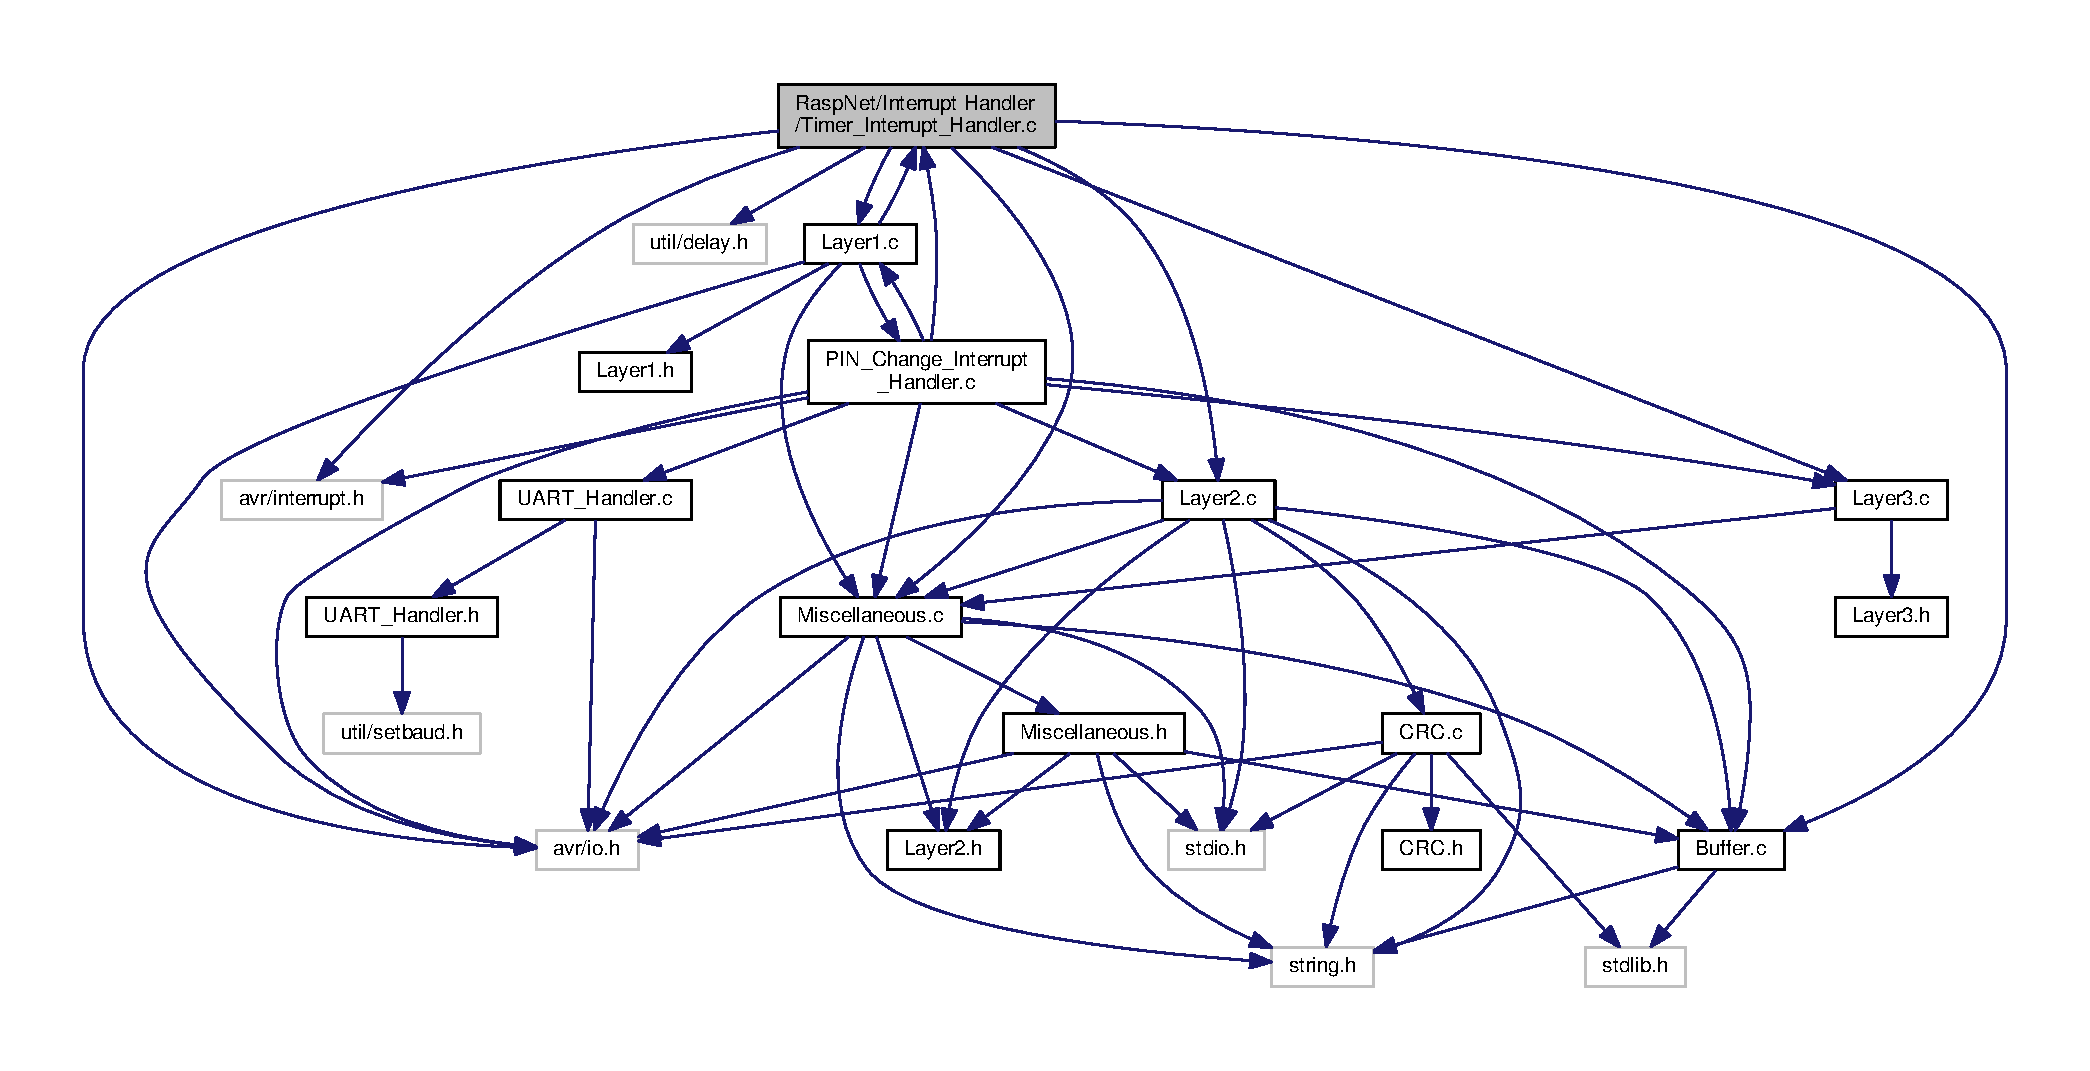
\includegraphics[width=350pt]{Timer__Interrupt__Handler_8c__incl}
\end{center}
\end{figure}
This graph shows which files directly or indirectly include this file\+:
\nopagebreak
\begin{figure}[H]
\begin{center}
\leavevmode
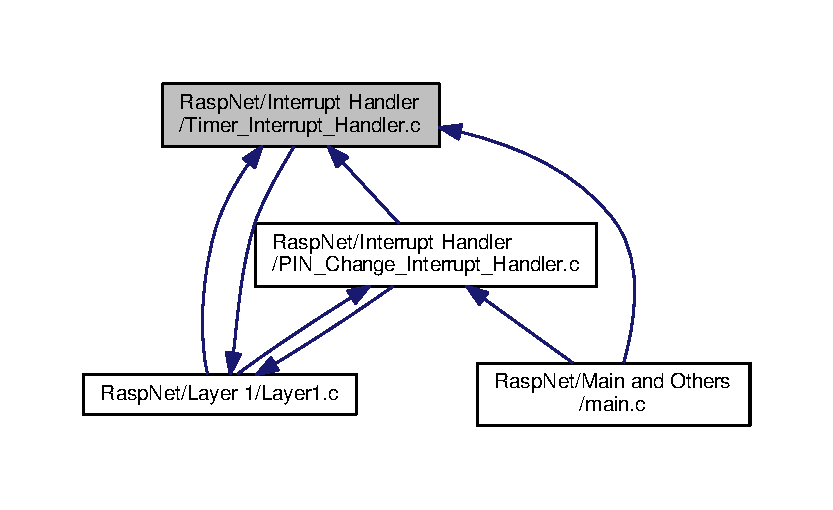
\includegraphics[width=350pt]{Timer__Interrupt__Handler_8c__dep__incl}
\end{center}
\end{figure}
\subsection*{Functions}
\begin{DoxyCompactItemize}
\item 
\hyperlink{Timer__Interrupt__Handler_8c_aec43762dc86e029b395d4e5819192c2d}{I\+SR} (T\+I\+M\+E\+R0\+\_\+\+C\+O\+M\+P\+A\+\_\+vect)
\end{DoxyCompactItemize}
\subsection*{Variables}
\begin{DoxyCompactItemize}
\item 
int \hyperlink{Timer__Interrupt__Handler_8c_a00da6a689ea15785d8f930576f3aeecd}{Transmit\+Index} =0
\item 
int \hyperlink{Timer__Interrupt__Handler_8c_a84100ed1f53f510ef91a3d88f24b4b53}{sender\+\_\+flag} =2
\item 
int \hyperlink{Timer__Interrupt__Handler_8c_ada6d325188acbfd053a663bad47ecda7}{array\+Index} =0
\item 
int \hyperlink{Timer__Interrupt__Handler_8c_a0b38a05fd17813ac9ded6c20924d8a76}{Compare\+\_\+A} =0
\item 
int \hyperlink{Timer__Interrupt__Handler_8c_a8b3219b9b8d2e090d4065a74c66635dc}{Compare\+\_\+B} =0
\end{DoxyCompactItemize}


\subsection{Function Documentation}
\index{Timer\+\_\+\+Interrupt\+\_\+\+Handler.\+c@{Timer\+\_\+\+Interrupt\+\_\+\+Handler.\+c}!I\+SR@{I\+SR}}
\index{I\+SR@{I\+SR}!Timer\+\_\+\+Interrupt\+\_\+\+Handler.\+c@{Timer\+\_\+\+Interrupt\+\_\+\+Handler.\+c}}
\subsubsection[{\texorpdfstring{I\+S\+R(\+T\+I\+M\+E\+R0\+\_\+\+C\+O\+M\+P\+A\+\_\+vect)}{ISR(TIMER0_COMPA_vect)}}]{\setlength{\rightskip}{0pt plus 5cm}I\+SR (
\begin{DoxyParamCaption}
\item[{T\+I\+M\+E\+R0\+\_\+\+C\+O\+M\+P\+A\+\_\+vect}]{}
\end{DoxyParamCaption}
)}\hypertarget{Timer__Interrupt__Handler_8c_aec43762dc86e029b395d4e5819192c2d}{}\label{Timer__Interrupt__Handler_8c_aec43762dc86e029b395d4e5819192c2d}
$<$ Check priority type

$<$ 1. Preamble transmit which is 8 bit data

$<$Set sending priority as normal 
\begin{DoxyCode}
22                        \{
23     \hyperlink{Timer__Interrupt__Handler_8c_a0b38a05fd17813ac9ded6c20924d8a76}{Compare\_A}=\hyperlink{Timer__Interrupt__Handler_8c_a0b38a05fd17813ac9ded6c20924d8a76}{Compare\_A}+1;
24     \textcolor{keywordflow}{if}(\hyperlink{Timer__Interrupt__Handler_8c_a0b38a05fd17813ac9ded6c20924d8a76}{Compare\_A}>100) \{
25         \hyperlink{Layer1_8c_a86a83b72f60ece554515ac4a4316dca6}{clock\_signal\_change}();
26         \_delay\_ms(1000);
27         \hyperlink{Timer__Interrupt__Handler_8c_a0b38a05fd17813ac9ded6c20924d8a76}{Compare\_A}=0;
29         \textcolor{keywordflow}{if}((\hyperlink{Layer3_8h_a2a0eb18d69ebbaf44dd4e863fa4f6a59}{priority\_type}==\hyperlink{Layer3_8h_a3b7ed14628679beda488dc3269b7b6a0}{priority\_for\_sending\_order}) ||(
      \hyperlink{Layer3_8h_a2a0eb18d69ebbaf44dd4e863fa4f6a59}{priority\_type}==\hyperlink{Layer3_8h_aaccf0a951ca84ac3578fa3bcfbac5522}{priority\_for\_relay})) \{
30             \textcolor{comment}{//\_delay\_ms(1000);}
32 \textcolor{comment}{}            \textcolor{keywordflow}{if}(\hyperlink{Timer__Interrupt__Handler_8c_a84100ed1f53f510ef91a3d88f24b4b53}{sender\_flag}==\hyperlink{Layer3_8h_a5b4f913d88d52723f970056a0ea4dd09}{transmit\_preamble}) \{
33                 \textcolor{keywordflow}{if}(\hyperlink{Miscellaneous_8c_a3c3d2514913829c2be8324680f0987b9}{read\_8\_bit}(\hyperlink{Buffer_8c_ac229f7d7f062771563514df9f3927eb6}{transmit\_packet\_pointer}->
      \hyperlink{structPacket_aa305c88136c91911a5159610863cb41d}{preamble},7-\hyperlink{Timer__Interrupt__Handler_8c_a00da6a689ea15785d8f930576f3aeecd}{TransmitIndex})) \{
34                     \hyperlink{Layer2_8c_ae785b505c564edf60c7c6a736235ddec}{tranmit\_1}();
35                 \}
36 
37                 \textcolor{keywordflow}{else} \textcolor{keywordflow}{if}(!\hyperlink{Miscellaneous_8c_a3c3d2514913829c2be8324680f0987b9}{read\_8\_bit}(\hyperlink{Buffer_8c_ac229f7d7f062771563514df9f3927eb6}{transmit\_packet\_pointer}->
      \hyperlink{structPacket_aa305c88136c91911a5159610863cb41d}{preamble},7-\hyperlink{Timer__Interrupt__Handler_8c_a00da6a689ea15785d8f930576f3aeecd}{TransmitIndex})) \{
38                     \hyperlink{Layer2_8c_ae79cf97d224edfd2ebfabc1a049360ce}{tranmit\_0}();
39                 \}
40                 \hyperlink{Timer__Interrupt__Handler_8c_a00da6a689ea15785d8f930576f3aeecd}{TransmitIndex}++;
41                 \textcolor{keywordflow}{if}(\hyperlink{Timer__Interrupt__Handler_8c_a00da6a689ea15785d8f930576f3aeecd}{TransmitIndex}>=8) \{
42                     \hyperlink{Timer__Interrupt__Handler_8c_a00da6a689ea15785d8f930576f3aeecd}{TransmitIndex}=0;
43                     \hyperlink{Miscellaneous_8c_afac087d6e168f5fc2cd8994eb07eadb2}{showLog}(\textcolor{stringliteral}{"Transmit Preamble: "});
44                     \hyperlink{Miscellaneous_8c_ae61d07597b559d7305b272b31507f138}{show\_8\_bit\_data}(\hyperlink{Buffer_8c_ac229f7d7f062771563514df9f3927eb6}{transmit\_packet\_pointer}->
      \hyperlink{structPacket_aa305c88136c91911a5159610863cb41d}{preamble});
45                     \hyperlink{Timer__Interrupt__Handler_8c_a84100ed1f53f510ef91a3d88f24b4b53}{sender\_flag}=\hyperlink{Layer3_8h_a97826fb6e7415b7cca5b6f704b2c37fc}{transmit\_crc};
46 
47                 \}
48 
49             \}
50 
52             \textcolor{keywordflow}{else} \textcolor{keywordflow}{if}(\hyperlink{Timer__Interrupt__Handler_8c_a84100ed1f53f510ef91a3d88f24b4b53}{sender\_flag}==\hyperlink{Layer3_8h_a97826fb6e7415b7cca5b6f704b2c37fc}{transmit\_crc}) \{
53                 \textcolor{keywordflow}{if}(\hyperlink{Miscellaneous_8c_a027b54125044a7b75a94ebdfef27ab46}{read\_32\_bit}(\hyperlink{Buffer_8c_ac229f7d7f062771563514df9f3927eb6}{transmit\_packet\_pointer}->
      \hyperlink{structPacket_abad95795e9615463d9d69d298a86b0b8}{crc},31-\hyperlink{Timer__Interrupt__Handler_8c_a00da6a689ea15785d8f930576f3aeecd}{TransmitIndex})) \{
54                     \hyperlink{Layer2_8c_ae785b505c564edf60c7c6a736235ddec}{tranmit\_1}();
55                 \}
56 
57                 \textcolor{keywordflow}{else} \textcolor{keywordflow}{if}(!\hyperlink{Miscellaneous_8c_a027b54125044a7b75a94ebdfef27ab46}{read\_32\_bit}(\hyperlink{Buffer_8c_ac229f7d7f062771563514df9f3927eb6}{transmit\_packet\_pointer}->
      \hyperlink{structPacket_abad95795e9615463d9d69d298a86b0b8}{crc},31-\hyperlink{Timer__Interrupt__Handler_8c_a00da6a689ea15785d8f930576f3aeecd}{TransmitIndex})) \{
58                     \hyperlink{Layer2_8c_ae79cf97d224edfd2ebfabc1a049360ce}{tranmit\_0}();
59                 \}
60                 \hyperlink{Timer__Interrupt__Handler_8c_a00da6a689ea15785d8f930576f3aeecd}{TransmitIndex}++;
61                 \textcolor{keywordflow}{if}(\hyperlink{Timer__Interrupt__Handler_8c_a00da6a689ea15785d8f930576f3aeecd}{TransmitIndex}>=32) \{
62                     \hyperlink{Miscellaneous_8c_afac087d6e168f5fc2cd8994eb07eadb2}{showLog}(\textcolor{stringliteral}{"Transmit CRC: "});
63                     \hyperlink{Timer__Interrupt__Handler_8c_a84100ed1f53f510ef91a3d88f24b4b53}{sender\_flag}=\hyperlink{Layer3_8h_a6b4b30550290df6d0f6c7726714672bf}{transmit\_payload\_size};
64                     \hyperlink{Miscellaneous_8c_a4da719f1865290663e587ffb1b00744d}{show\_32\_bit\_data}(\hyperlink{Buffer_8c_ac229f7d7f062771563514df9f3927eb6}{transmit\_packet\_pointer}->
      \hyperlink{structPacket_abad95795e9615463d9d69d298a86b0b8}{crc});
65                     \hyperlink{Timer__Interrupt__Handler_8c_a00da6a689ea15785d8f930576f3aeecd}{TransmitIndex}=0;
66                 \}
67 
68             \}
69 
71             \textcolor{keywordflow}{else} \textcolor{keywordflow}{if}(\hyperlink{Timer__Interrupt__Handler_8c_a84100ed1f53f510ef91a3d88f24b4b53}{sender\_flag}==\hyperlink{Layer3_8h_a6b4b30550290df6d0f6c7726714672bf}{transmit\_payload\_size}) \{
72                 \textcolor{keywordflow}{if}(\hyperlink{Miscellaneous_8c_a3c3d2514913829c2be8324680f0987b9}{read\_8\_bit}(\hyperlink{Buffer_8c_ac229f7d7f062771563514df9f3927eb6}{transmit\_packet\_pointer}->
      \hyperlink{structPacket_ab13014675ea9eda122b1c50842a567fc}{payload\_siz},7-\hyperlink{Timer__Interrupt__Handler_8c_a00da6a689ea15785d8f930576f3aeecd}{TransmitIndex})) \{
73                     \hyperlink{Layer2_8c_ae785b505c564edf60c7c6a736235ddec}{tranmit\_1}();
74 
75                 \}
76 
77                 \textcolor{keywordflow}{else} \textcolor{keywordflow}{if}(!\hyperlink{Miscellaneous_8c_a3c3d2514913829c2be8324680f0987b9}{read\_8\_bit}(\hyperlink{Buffer_8c_ac229f7d7f062771563514df9f3927eb6}{transmit\_packet\_pointer}->
      \hyperlink{structPacket_ab13014675ea9eda122b1c50842a567fc}{payload\_siz},7-\hyperlink{Timer__Interrupt__Handler_8c_a00da6a689ea15785d8f930576f3aeecd}{TransmitIndex})) \{
78                     \hyperlink{Layer2_8c_ae79cf97d224edfd2ebfabc1a049360ce}{tranmit\_0}();
79 
80                 \}
81                 \hyperlink{Timer__Interrupt__Handler_8c_a00da6a689ea15785d8f930576f3aeecd}{TransmitIndex}++;
82                 \textcolor{keywordflow}{if}(\hyperlink{Timer__Interrupt__Handler_8c_a00da6a689ea15785d8f930576f3aeecd}{TransmitIndex}>=8) \{
83                     \hyperlink{Miscellaneous_8c_afac087d6e168f5fc2cd8994eb07eadb2}{showLog}(\textcolor{stringliteral}{"Payload size send: "});
84                     \hyperlink{Miscellaneous_8c_ae61d07597b559d7305b272b31507f138}{show\_8\_bit\_data}(\hyperlink{Buffer_8c_ac229f7d7f062771563514df9f3927eb6}{transmit\_packet\_pointer}->
      \hyperlink{structPacket_ab13014675ea9eda122b1c50842a567fc}{payload\_siz});
85                     \hyperlink{Timer__Interrupt__Handler_8c_a00da6a689ea15785d8f930576f3aeecd}{TransmitIndex}=0;
86                     \hyperlink{Timer__Interrupt__Handler_8c_a84100ed1f53f510ef91a3d88f24b4b53}{sender\_flag}=\hyperlink{Layer3_8h_a44e78cb310dd2d291b3d3f96c2a4fbf3}{transmit\_destination\_address};
87                 \}
88             \}
89 
91             \textcolor{keywordflow}{else} \textcolor{keywordflow}{if}(\hyperlink{Timer__Interrupt__Handler_8c_a84100ed1f53f510ef91a3d88f24b4b53}{sender\_flag}==\hyperlink{Layer3_8h_a44e78cb310dd2d291b3d3f96c2a4fbf3}{transmit\_destination\_address}) \{
92                 \textcolor{keywordflow}{if}(\hyperlink{Miscellaneous_8c_a3c3d2514913829c2be8324680f0987b9}{read\_8\_bit}(\hyperlink{Buffer_8c_ac229f7d7f062771563514df9f3927eb6}{transmit\_packet\_pointer}->
      \hyperlink{structPacket_af626fe07d93fe4116d613304792df080}{destination},7-\hyperlink{Timer__Interrupt__Handler_8c_a00da6a689ea15785d8f930576f3aeecd}{TransmitIndex})) \{
93                     \hyperlink{Layer2_8c_ae785b505c564edf60c7c6a736235ddec}{tranmit\_1}();
94                 \}
95 
96                 \textcolor{keywordflow}{else} \textcolor{keywordflow}{if}(!\hyperlink{Miscellaneous_8c_a3c3d2514913829c2be8324680f0987b9}{read\_8\_bit}(\hyperlink{Buffer_8c_ac229f7d7f062771563514df9f3927eb6}{transmit\_packet\_pointer}->
      \hyperlink{structPacket_af626fe07d93fe4116d613304792df080}{destination},7-\hyperlink{Timer__Interrupt__Handler_8c_a00da6a689ea15785d8f930576f3aeecd}{TransmitIndex})) \{
97                     \hyperlink{Layer2_8c_ae79cf97d224edfd2ebfabc1a049360ce}{tranmit\_0}();
98                 \}
99                 \hyperlink{Timer__Interrupt__Handler_8c_a00da6a689ea15785d8f930576f3aeecd}{TransmitIndex}++;
100                 \textcolor{keywordflow}{if}(\hyperlink{Timer__Interrupt__Handler_8c_a00da6a689ea15785d8f930576f3aeecd}{TransmitIndex}>=8) \{
101                     \hyperlink{Miscellaneous_8c_afac087d6e168f5fc2cd8994eb07eadb2}{showLog}(\textcolor{stringliteral}{"\(\backslash\)nDestination address send\(\backslash\)n"});
102                     \hyperlink{Miscellaneous_8c_ae61d07597b559d7305b272b31507f138}{show\_8\_bit\_data}(\hyperlink{Buffer_8c_ac229f7d7f062771563514df9f3927eb6}{transmit\_packet\_pointer}->
      \hyperlink{structPacket_af626fe07d93fe4116d613304792df080}{destination});
103                     \hyperlink{Timer__Interrupt__Handler_8c_a84100ed1f53f510ef91a3d88f24b4b53}{sender\_flag}=\hyperlink{Layer3_8h_aa4e2ceb5bd48f2fde7e6c7240ca66e44}{transmit\_source\_address};
104                     \hyperlink{Timer__Interrupt__Handler_8c_a00da6a689ea15785d8f930576f3aeecd}{TransmitIndex}=0;
105                 \}
106 
107             \}
108 
110             \textcolor{keywordflow}{else} \textcolor{keywordflow}{if}(\hyperlink{Timer__Interrupt__Handler_8c_a84100ed1f53f510ef91a3d88f24b4b53}{sender\_flag}==\hyperlink{Layer3_8h_aa4e2ceb5bd48f2fde7e6c7240ca66e44}{transmit\_source\_address}) \{
111                 \textcolor{keywordflow}{if}(\hyperlink{Miscellaneous_8c_a3c3d2514913829c2be8324680f0987b9}{read\_8\_bit}(\hyperlink{Buffer_8c_ac229f7d7f062771563514df9f3927eb6}{transmit\_packet\_pointer}->
      \hyperlink{structPacket_a01308f5b690e5060fea6037e765058b9}{source},7-\hyperlink{Timer__Interrupt__Handler_8c_a00da6a689ea15785d8f930576f3aeecd}{TransmitIndex})) \{
112                     \hyperlink{Layer2_8c_ae785b505c564edf60c7c6a736235ddec}{tranmit\_1}();
113                 \}
114                 \textcolor{keywordflow}{else} \textcolor{keywordflow}{if}(!\hyperlink{Miscellaneous_8c_a3c3d2514913829c2be8324680f0987b9}{read\_8\_bit}(\hyperlink{Buffer_8c_ac229f7d7f062771563514df9f3927eb6}{transmit\_packet\_pointer}->
      \hyperlink{structPacket_a01308f5b690e5060fea6037e765058b9}{source},7-\hyperlink{Timer__Interrupt__Handler_8c_a00da6a689ea15785d8f930576f3aeecd}{TransmitIndex})) \{
115                     \hyperlink{Layer2_8c_ae79cf97d224edfd2ebfabc1a049360ce}{tranmit\_0}();
116                 \}
117                 \hyperlink{Timer__Interrupt__Handler_8c_a00da6a689ea15785d8f930576f3aeecd}{TransmitIndex}++;
118                 \textcolor{keywordflow}{if}(\hyperlink{Timer__Interrupt__Handler_8c_a00da6a689ea15785d8f930576f3aeecd}{TransmitIndex}>=8) \{
119                     \hyperlink{Miscellaneous_8c_afac087d6e168f5fc2cd8994eb07eadb2}{showLog}(\textcolor{stringliteral}{"\(\backslash\)nSource address send\(\backslash\)n"});
120                     \hyperlink{Timer__Interrupt__Handler_8c_a84100ed1f53f510ef91a3d88f24b4b53}{sender\_flag}=\hyperlink{Layer3_8h_afde148ebf464f31e83576556e5bc4102}{transmit\_payload};
121                     \hyperlink{Miscellaneous_8c_ae61d07597b559d7305b272b31507f138}{show\_8\_bit\_data}(\hyperlink{Buffer_8c_ac229f7d7f062771563514df9f3927eb6}{transmit\_packet\_pointer}->
      \hyperlink{structPacket_a01308f5b690e5060fea6037e765058b9}{source});
122                     \hyperlink{Timer__Interrupt__Handler_8c_a00da6a689ea15785d8f930576f3aeecd}{TransmitIndex}=0;
123                     \hyperlink{Timer__Interrupt__Handler_8c_ada6d325188acbfd053a663bad47ecda7}{arrayIndex}=2;
124                 \}
125 
126             \}
127 
129             \textcolor{keywordflow}{else} \textcolor{keywordflow}{if}(\hyperlink{Timer__Interrupt__Handler_8c_a84100ed1f53f510ef91a3d88f24b4b53}{sender\_flag}==\hyperlink{Layer3_8h_afde148ebf464f31e83576556e5bc4102}{transmit\_payload}) \{
130 
131                 \textcolor{keywordflow}{if}(\hyperlink{Miscellaneous_8c_a3c3d2514913829c2be8324680f0987b9}{read\_8\_bit}(\hyperlink{Buffer_8c_ac229f7d7f062771563514df9f3927eb6}{transmit\_packet\_pointer}->
      \hyperlink{structPacket_a58a48ac639979f488f254bbcb98e72b8}{payload}[\hyperlink{Timer__Interrupt__Handler_8c_ada6d325188acbfd053a663bad47ecda7}{arrayIndex}],(7-(\hyperlink{Timer__Interrupt__Handler_8c_a00da6a689ea15785d8f930576f3aeecd}{TransmitIndex}%8)))) \{
132                     \hyperlink{Layer2_8c_ae785b505c564edf60c7c6a736235ddec}{tranmit\_1}();
133                 \}
134 
135                 \textcolor{keywordflow}{else} \textcolor{keywordflow}{if}(!\hyperlink{Miscellaneous_8c_a3c3d2514913829c2be8324680f0987b9}{read\_8\_bit}(\hyperlink{Buffer_8c_ac229f7d7f062771563514df9f3927eb6}{transmit\_packet\_pointer}->
      \hyperlink{structPacket_a58a48ac639979f488f254bbcb98e72b8}{payload}[\hyperlink{Timer__Interrupt__Handler_8c_ada6d325188acbfd053a663bad47ecda7}{arrayIndex}],(7-(\hyperlink{Timer__Interrupt__Handler_8c_a00da6a689ea15785d8f930576f3aeecd}{TransmitIndex}%8)))) \{
136                     \hyperlink{Layer2_8c_ae79cf97d224edfd2ebfabc1a049360ce}{tranmit\_0}();
137                 \}
138                 \hyperlink{Timer__Interrupt__Handler_8c_a00da6a689ea15785d8f930576f3aeecd}{TransmitIndex}++;
139                 \textcolor{keywordflow}{if}(\hyperlink{Timer__Interrupt__Handler_8c_a00da6a689ea15785d8f930576f3aeecd}{TransmitIndex}%8==0) \{
140                     \hyperlink{Timer__Interrupt__Handler_8c_ada6d325188acbfd053a663bad47ecda7}{arrayIndex}=\hyperlink{Timer__Interrupt__Handler_8c_ada6d325188acbfd053a663bad47ecda7}{arrayIndex}+1;
141 
142                 \}
143 
144                 \textcolor{keywordflow}{if}(\hyperlink{Timer__Interrupt__Handler_8c_a00da6a689ea15785d8f930576f3aeecd}{TransmitIndex}>=(((\hyperlink{Buffer_8c_ac229f7d7f062771563514df9f3927eb6}{transmit\_packet\_pointer}->
      \hyperlink{structPacket_ab13014675ea9eda122b1c50842a567fc}{payload\_siz})-2)*8)) \{
145                     \hyperlink{Miscellaneous_8c_afac087d6e168f5fc2cd8994eb07eadb2}{showLog}(\textcolor{stringliteral}{"Send payload: "});
146                     \hyperlink{Miscellaneous_8c_a9ea1d4b6a27b5caa55c150b2ba17983a}{show\_payload}(\hyperlink{Buffer_8c_ac229f7d7f062771563514df9f3927eb6}{transmit\_packet\_pointer}->
      \hyperlink{structPacket_a58a48ac639979f488f254bbcb98e72b8}{payload},\hyperlink{Buffer_8c_ac229f7d7f062771563514df9f3927eb6}{transmit\_packet\_pointer}->\hyperlink{structPacket_ab13014675ea9eda122b1c50842a567fc}{payload\_siz}*8);
147                     \hyperlink{Timer__Interrupt__Handler_8c_a00da6a689ea15785d8f930576f3aeecd}{TransmitIndex}=0;
148                     \textcolor{keywordflow}{if}(\hyperlink{Layer3_8h_a2a0eb18d69ebbaf44dd4e863fa4f6a59}{priority\_type}==\hyperlink{Layer3_8h_a3b7ed14628679beda488dc3269b7b6a0}{priority\_for\_sending\_order}) \{
149                         \hyperlink{Miscellaneous_8c_afac087d6e168f5fc2cd8994eb07eadb2}{showLog}(\textcolor{stringliteral}{"Transmitted....!"});
150 
151                     \}
152 
153                     \hyperlink{Layer3_8h_a2a0eb18d69ebbaf44dd4e863fa4f6a59}{priority\_type}=\hyperlink{Layer3_8h_afd5191a3ada0a4968402449c806bd4b3}{priority\_normal}; 
154                     \hyperlink{Layer3_8c_a5cc35a45674625cd8733379d3f0523b8}{discard\_packet}(\hyperlink{Buffer_8c_ac229f7d7f062771563514df9f3927eb6}{transmit\_packet\_pointer});
155                     \hyperlink{Timer__Interrupt__Handler_8c_a84100ed1f53f510ef91a3d88f24b4b53}{sender\_flag}=\hyperlink{Layer3_8h_af43b7652801ee9e083162514d5372e9f}{transmitted};
156                     \hyperlink{Miscellaneous_8c_afac087d6e168f5fc2cd8994eb07eadb2}{showLog}(\textcolor{stringliteral}{"----------------transmit cycle finish----------------------"});
157 
158                 \}
159 
160 
161             \}
162 
163         \}
164 
165     \}
166 
167 \}
\end{DoxyCode}


\subsection{Variable Documentation}
\index{Timer\+\_\+\+Interrupt\+\_\+\+Handler.\+c@{Timer\+\_\+\+Interrupt\+\_\+\+Handler.\+c}!array\+Index@{array\+Index}}
\index{array\+Index@{array\+Index}!Timer\+\_\+\+Interrupt\+\_\+\+Handler.\+c@{Timer\+\_\+\+Interrupt\+\_\+\+Handler.\+c}}
\subsubsection[{\texorpdfstring{array\+Index}{arrayIndex}}]{\setlength{\rightskip}{0pt plus 5cm}int array\+Index =0}\hypertarget{Timer__Interrupt__Handler_8c_ada6d325188acbfd053a663bad47ecda7}{}\label{Timer__Interrupt__Handler_8c_ada6d325188acbfd053a663bad47ecda7}
\index{Timer\+\_\+\+Interrupt\+\_\+\+Handler.\+c@{Timer\+\_\+\+Interrupt\+\_\+\+Handler.\+c}!Compare\+\_\+A@{Compare\+\_\+A}}
\index{Compare\+\_\+A@{Compare\+\_\+A}!Timer\+\_\+\+Interrupt\+\_\+\+Handler.\+c@{Timer\+\_\+\+Interrupt\+\_\+\+Handler.\+c}}
\subsubsection[{\texorpdfstring{Compare\+\_\+A}{Compare_A}}]{\setlength{\rightskip}{0pt plus 5cm}int Compare\+\_\+A =0}\hypertarget{Timer__Interrupt__Handler_8c_a0b38a05fd17813ac9ded6c20924d8a76}{}\label{Timer__Interrupt__Handler_8c_a0b38a05fd17813ac9ded6c20924d8a76}
\index{Timer\+\_\+\+Interrupt\+\_\+\+Handler.\+c@{Timer\+\_\+\+Interrupt\+\_\+\+Handler.\+c}!Compare\+\_\+B@{Compare\+\_\+B}}
\index{Compare\+\_\+B@{Compare\+\_\+B}!Timer\+\_\+\+Interrupt\+\_\+\+Handler.\+c@{Timer\+\_\+\+Interrupt\+\_\+\+Handler.\+c}}
\subsubsection[{\texorpdfstring{Compare\+\_\+B}{Compare_B}}]{\setlength{\rightskip}{0pt plus 5cm}int Compare\+\_\+B =0}\hypertarget{Timer__Interrupt__Handler_8c_a8b3219b9b8d2e090d4065a74c66635dc}{}\label{Timer__Interrupt__Handler_8c_a8b3219b9b8d2e090d4065a74c66635dc}
Timer interrupt for transmitting data \index{Timer\+\_\+\+Interrupt\+\_\+\+Handler.\+c@{Timer\+\_\+\+Interrupt\+\_\+\+Handler.\+c}!sender\+\_\+flag@{sender\+\_\+flag}}
\index{sender\+\_\+flag@{sender\+\_\+flag}!Timer\+\_\+\+Interrupt\+\_\+\+Handler.\+c@{Timer\+\_\+\+Interrupt\+\_\+\+Handler.\+c}}
\subsubsection[{\texorpdfstring{sender\+\_\+flag}{sender_flag}}]{\setlength{\rightskip}{0pt plus 5cm}int sender\+\_\+flag =2}\hypertarget{Timer__Interrupt__Handler_8c_a84100ed1f53f510ef91a3d88f24b4b53}{}\label{Timer__Interrupt__Handler_8c_a84100ed1f53f510ef91a3d88f24b4b53}
\index{Timer\+\_\+\+Interrupt\+\_\+\+Handler.\+c@{Timer\+\_\+\+Interrupt\+\_\+\+Handler.\+c}!Transmit\+Index@{Transmit\+Index}}
\index{Transmit\+Index@{Transmit\+Index}!Timer\+\_\+\+Interrupt\+\_\+\+Handler.\+c@{Timer\+\_\+\+Interrupt\+\_\+\+Handler.\+c}}
\subsubsection[{\texorpdfstring{Transmit\+Index}{TransmitIndex}}]{\setlength{\rightskip}{0pt plus 5cm}int Transmit\+Index =0}\hypertarget{Timer__Interrupt__Handler_8c_a00da6a689ea15785d8f930576f3aeecd}{}\label{Timer__Interrupt__Handler_8c_a00da6a689ea15785d8f930576f3aeecd}

\hypertarget{Layer1_8c}{}\section{Rasp\+Net/\+Layer 1/\+Layer1.c File Reference}
\label{Layer1_8c}\index{Rasp\+Net/\+Layer 1/\+Layer1.\+c@{Rasp\+Net/\+Layer 1/\+Layer1.\+c}}
{\ttfamily \#include $<$avr/io.\+h$>$}\\*
{\ttfamily \#include \char`\"{}Timer\+\_\+\+Interrupt\+\_\+\+Handler.\+c\char`\"{}}\\*
{\ttfamily \#include \char`\"{}P\+I\+N\+\_\+\+Change\+\_\+\+Interrupt\+\_\+\+Handler.\+c\char`\"{}}\\*
{\ttfamily \#include \char`\"{}Layer1.\+h\char`\"{}}\\*
{\ttfamily \#include \char`\"{}Miscellaneous.\+c\char`\"{}}\\*
Include dependency graph for Layer1.\+c\+:
\nopagebreak
\begin{figure}[H]
\begin{center}
\leavevmode
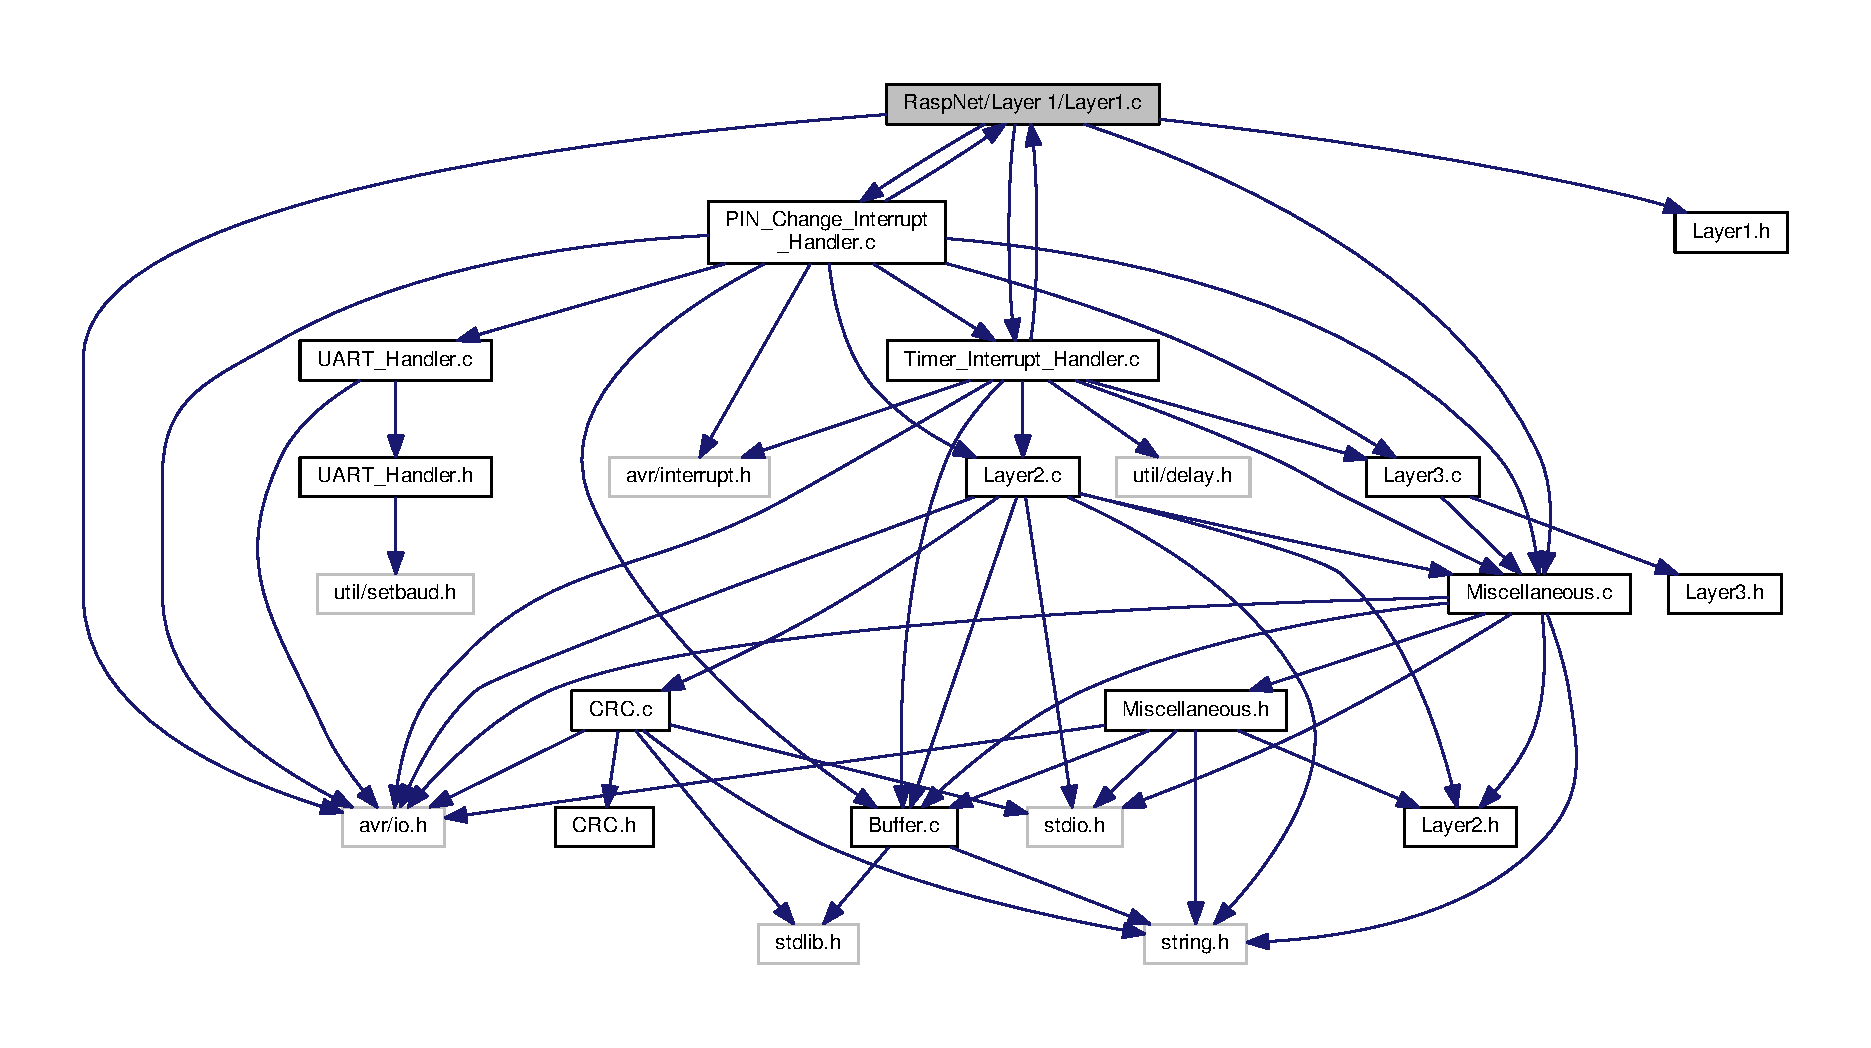
\includegraphics[width=350pt]{Layer1_8c__incl}
\end{center}
\end{figure}
This graph shows which files directly or indirectly include this file\+:
\nopagebreak
\begin{figure}[H]
\begin{center}
\leavevmode
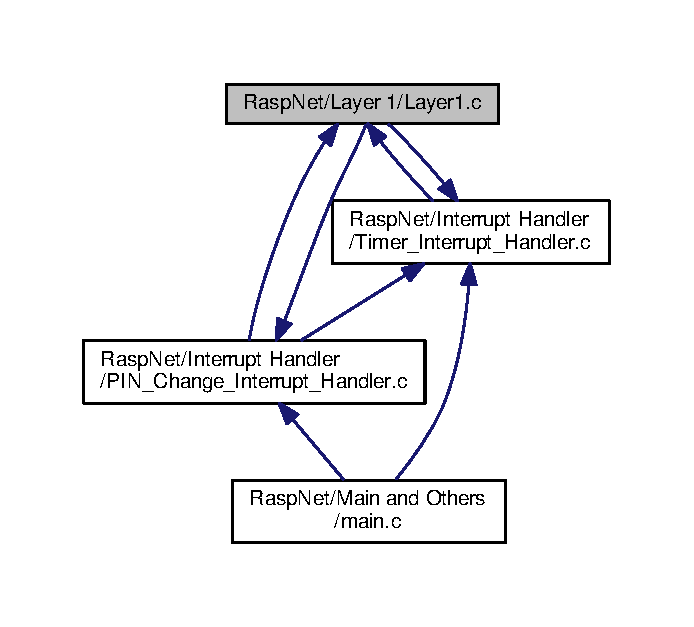
\includegraphics[width=333pt]{Layer1_8c__dep__incl}
\end{center}
\end{figure}
\subsection*{Functions}
\begin{DoxyCompactItemize}
\item 
void \hyperlink{Layer1_8c_a229b2097a7d8df6649528de6108edb54}{L\+E\+D\+\_\+blink\+\_\+for\+\_\+clock\+\_\+signal\+\_\+receive} ()
\begin{DoxyCompactList}\small\item\em This functions is used for debugging purpose L\+ED blinks based on clock signal. \end{DoxyCompactList}\item 
void \hyperlink{Layer1_8c_a2081bb4779c7101b51f8572e20fab5e3}{L\+E\+D\+\_\+blink\+\_\+for\+\_\+data\+\_\+signal\+\_\+receive} ()
\begin{DoxyCompactList}\small\item\em This functions is used for debugging purpose L\+ED blinks based on data signal. \end{DoxyCompactList}\item 
void \hyperlink{Layer1_8c_a86a83b72f60ece554515ac4a4316dca6}{clock\+\_\+signal\+\_\+change} ()
\begin{DoxyCompactList}\small\item\em Change clock signal\+: from high(1) to low(0), low(0) to high(1) \end{DoxyCompactList}\item 
void \hyperlink{Layer1_8c_abf739cbeeff67b31459f8899e02986b0}{clock\+\_\+signal\+\_\+receive} ()
\begin{DoxyCompactList}\small\item\em Receive the clock signal when the clock signal is changed, then a new bit. \end{DoxyCompactList}\end{DoxyCompactItemize}


\subsection{Function Documentation}
\index{Layer1.\+c@{Layer1.\+c}!clock\+\_\+signal\+\_\+change@{clock\+\_\+signal\+\_\+change}}
\index{clock\+\_\+signal\+\_\+change@{clock\+\_\+signal\+\_\+change}!Layer1.\+c@{Layer1.\+c}}
\subsubsection[{\texorpdfstring{clock\+\_\+signal\+\_\+change()}{clock_signal_change()}}]{\setlength{\rightskip}{0pt plus 5cm}void clock\+\_\+signal\+\_\+change (
\begin{DoxyParamCaption}
{}
\end{DoxyParamCaption}
)}\hypertarget{Layer1_8c_a86a83b72f60ece554515ac4a4316dca6}{}\label{Layer1_8c_a86a83b72f60ece554515ac4a4316dca6}


Change clock signal\+: from high(1) to low(0), low(0) to high(1) 

\begin{DoxyReturn}{Returns}
void nothing has to return from this function 
\end{DoxyReturn}
$<$ if clock signal is H\+I\+GH,then make it L\+OW

$<$ if clock signal is L\+OW,then make it H\+I\+GH 
\begin{DoxyCode}
19                            \{
20     
21     \textcolor{keywordflow}{if}(PINB & (1<<PB4)) \{
22         PORTB&=~(1<<PB4); 
23     \}
24     \textcolor{keywordflow}{else} \{
25         PORTB|=(1<<PB4); 
26     \}
27 
28 \}
\end{DoxyCode}
\index{Layer1.\+c@{Layer1.\+c}!clock\+\_\+signal\+\_\+receive@{clock\+\_\+signal\+\_\+receive}}
\index{clock\+\_\+signal\+\_\+receive@{clock\+\_\+signal\+\_\+receive}!Layer1.\+c@{Layer1.\+c}}
\subsubsection[{\texorpdfstring{clock\+\_\+signal\+\_\+receive()}{clock_signal_receive()}}]{\setlength{\rightskip}{0pt plus 5cm}void clock\+\_\+signal\+\_\+receive (
\begin{DoxyParamCaption}
{}
\end{DoxyParamCaption}
)}\hypertarget{Layer1_8c_abf739cbeeff67b31459f8899e02986b0}{}\label{Layer1_8c_abf739cbeeff67b31459f8899e02986b0}


Receive the clock signal when the clock signal is changed, then a new bit. 

is available in the data pin for reading \begin{DoxyReturn}{Returns}
void nothing has to return from this function 
\end{DoxyReturn}
$<$ Used for debugging purpose 
\begin{DoxyCode}
31                             \{
32     \hyperlink{Layer1_8c_a229b2097a7d8df6649528de6108edb54}{LED\_blink\_for\_clock\_signal\_receive}(); 
33 \}
\end{DoxyCode}
\index{Layer1.\+c@{Layer1.\+c}!L\+E\+D\+\_\+blink\+\_\+for\+\_\+clock\+\_\+signal\+\_\+receive@{L\+E\+D\+\_\+blink\+\_\+for\+\_\+clock\+\_\+signal\+\_\+receive}}
\index{L\+E\+D\+\_\+blink\+\_\+for\+\_\+clock\+\_\+signal\+\_\+receive@{L\+E\+D\+\_\+blink\+\_\+for\+\_\+clock\+\_\+signal\+\_\+receive}!Layer1.\+c@{Layer1.\+c}}
\subsubsection[{\texorpdfstring{L\+E\+D\+\_\+blink\+\_\+for\+\_\+clock\+\_\+signal\+\_\+receive()}{LED_blink_for_clock_signal_receive()}}]{\setlength{\rightskip}{0pt plus 5cm}void L\+E\+D\+\_\+blink\+\_\+for\+\_\+clock\+\_\+signal\+\_\+receive (
\begin{DoxyParamCaption}
{}
\end{DoxyParamCaption}
)}\hypertarget{Layer1_8c_a229b2097a7d8df6649528de6108edb54}{}\label{Layer1_8c_a229b2097a7d8df6649528de6108edb54}


This functions is used for debugging purpose L\+ED blinks based on clock signal. 

\begin{DoxyReturn}{Returns}
void nothing has to return from this function 
\end{DoxyReturn}
$<$ L\+ED toggle based on clock signal receive 
\begin{DoxyCode}
10                                           \{
11     PORTB^=(1<<PB3); 
12 \}
\end{DoxyCode}
\index{Layer1.\+c@{Layer1.\+c}!L\+E\+D\+\_\+blink\+\_\+for\+\_\+data\+\_\+signal\+\_\+receive@{L\+E\+D\+\_\+blink\+\_\+for\+\_\+data\+\_\+signal\+\_\+receive}}
\index{L\+E\+D\+\_\+blink\+\_\+for\+\_\+data\+\_\+signal\+\_\+receive@{L\+E\+D\+\_\+blink\+\_\+for\+\_\+data\+\_\+signal\+\_\+receive}!Layer1.\+c@{Layer1.\+c}}
\subsubsection[{\texorpdfstring{L\+E\+D\+\_\+blink\+\_\+for\+\_\+data\+\_\+signal\+\_\+receive()}{LED_blink_for_data_signal_receive()}}]{\setlength{\rightskip}{0pt plus 5cm}void L\+E\+D\+\_\+blink\+\_\+for\+\_\+data\+\_\+signal\+\_\+receive (
\begin{DoxyParamCaption}
{}
\end{DoxyParamCaption}
)}\hypertarget{Layer1_8c_a2081bb4779c7101b51f8572e20fab5e3}{}\label{Layer1_8c_a2081bb4779c7101b51f8572e20fab5e3}


This functions is used for debugging purpose L\+ED blinks based on data signal. 

\begin{DoxyReturn}{Returns}
void nothing has to return from this function 
\end{DoxyReturn}
$<$ L\+ED toggle based on data signal receive 
\begin{DoxyCode}
14                                          \{
15     PORTB^=(1<<PB2); 
16 \}
\end{DoxyCode}

\hypertarget{Layer1_8h}{}\section{Rasp\+Net/\+Layer 1/\+Layer1.h File Reference}
\label{Layer1_8h}\index{Rasp\+Net/\+Layer 1/\+Layer1.\+h@{Rasp\+Net/\+Layer 1/\+Layer1.\+h}}
This graph shows which files directly or indirectly include this file\+:
\nopagebreak
\begin{figure}[H]
\begin{center}
\leavevmode
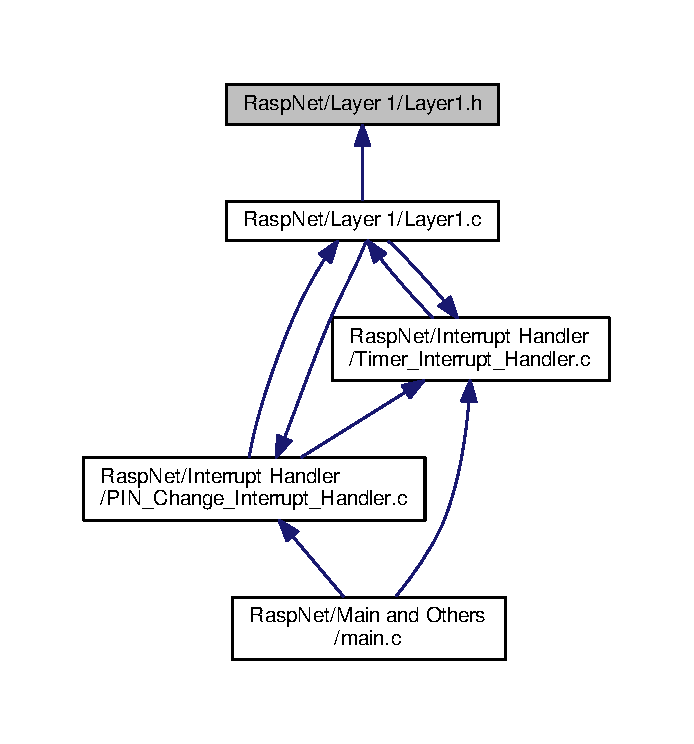
\includegraphics[width=333pt]{Layer1_8h__dep__incl}
\end{center}
\end{figure}
\subsection*{Functions}
\begin{DoxyCompactItemize}
\item 
void \hyperlink{Layer1_8h_a229b2097a7d8df6649528de6108edb54}{L\+E\+D\+\_\+blink\+\_\+for\+\_\+clock\+\_\+signal\+\_\+receive} ()
\begin{DoxyCompactList}\small\item\em This functions is used for debugging purpose L\+ED blinks based on clock signal. \end{DoxyCompactList}\item 
void \hyperlink{Layer1_8h_a2081bb4779c7101b51f8572e20fab5e3}{L\+E\+D\+\_\+blink\+\_\+for\+\_\+data\+\_\+signal\+\_\+receive} ()
\begin{DoxyCompactList}\small\item\em This functions is used for debugging purpose L\+ED blinks based on data signal. \end{DoxyCompactList}\item 
void \hyperlink{Layer1_8h_a86a83b72f60ece554515ac4a4316dca6}{clock\+\_\+signal\+\_\+change} ()
\begin{DoxyCompactList}\small\item\em Change clock signal\+: from high(1) to low(0), low(0) to high(1) \end{DoxyCompactList}\item 
void \hyperlink{Layer1_8h_abf739cbeeff67b31459f8899e02986b0}{clock\+\_\+signal\+\_\+receive} ()
\begin{DoxyCompactList}\small\item\em Receive the clock signal when the clock signal is changed, then a new bit. \end{DoxyCompactList}\end{DoxyCompactItemize}


\subsection{Function Documentation}
\index{Layer1.\+h@{Layer1.\+h}!clock\+\_\+signal\+\_\+change@{clock\+\_\+signal\+\_\+change}}
\index{clock\+\_\+signal\+\_\+change@{clock\+\_\+signal\+\_\+change}!Layer1.\+h@{Layer1.\+h}}
\subsubsection[{\texorpdfstring{clock\+\_\+signal\+\_\+change()}{clock_signal_change()}}]{\setlength{\rightskip}{0pt plus 5cm}void clock\+\_\+signal\+\_\+change (
\begin{DoxyParamCaption}
{}
\end{DoxyParamCaption}
)}\hypertarget{Layer1_8h_a86a83b72f60ece554515ac4a4316dca6}{}\label{Layer1_8h_a86a83b72f60ece554515ac4a4316dca6}


Change clock signal\+: from high(1) to low(0), low(0) to high(1) 

\begin{DoxyReturn}{Returns}
void nothing has to return from this function 
\end{DoxyReturn}
$<$ if clock signal is H\+I\+GH,then make it L\+OW

$<$ if clock signal is L\+OW,then make it H\+I\+GH 
\begin{DoxyCode}
19                            \{
20     
21     \textcolor{keywordflow}{if}(PINB & (1<<PB4)) \{
22         PORTB&=~(1<<PB4); 
23     \}
24     \textcolor{keywordflow}{else} \{
25         PORTB|=(1<<PB4); 
26     \}
27 
28 \}
\end{DoxyCode}
\index{Layer1.\+h@{Layer1.\+h}!clock\+\_\+signal\+\_\+receive@{clock\+\_\+signal\+\_\+receive}}
\index{clock\+\_\+signal\+\_\+receive@{clock\+\_\+signal\+\_\+receive}!Layer1.\+h@{Layer1.\+h}}
\subsubsection[{\texorpdfstring{clock\+\_\+signal\+\_\+receive()}{clock_signal_receive()}}]{\setlength{\rightskip}{0pt plus 5cm}void clock\+\_\+signal\+\_\+receive (
\begin{DoxyParamCaption}
{}
\end{DoxyParamCaption}
)}\hypertarget{Layer1_8h_abf739cbeeff67b31459f8899e02986b0}{}\label{Layer1_8h_abf739cbeeff67b31459f8899e02986b0}


Receive the clock signal when the clock signal is changed, then a new bit. 

is available in the data pin for reading \begin{DoxyReturn}{Returns}
void nothing has to return from this function 
\end{DoxyReturn}
$<$ Used for debugging purpose 
\begin{DoxyCode}
31                             \{
32     \hyperlink{Layer1_8c_a229b2097a7d8df6649528de6108edb54}{LED\_blink\_for\_clock\_signal\_receive}(); 
33 \}
\end{DoxyCode}
\index{Layer1.\+h@{Layer1.\+h}!L\+E\+D\+\_\+blink\+\_\+for\+\_\+clock\+\_\+signal\+\_\+receive@{L\+E\+D\+\_\+blink\+\_\+for\+\_\+clock\+\_\+signal\+\_\+receive}}
\index{L\+E\+D\+\_\+blink\+\_\+for\+\_\+clock\+\_\+signal\+\_\+receive@{L\+E\+D\+\_\+blink\+\_\+for\+\_\+clock\+\_\+signal\+\_\+receive}!Layer1.\+h@{Layer1.\+h}}
\subsubsection[{\texorpdfstring{L\+E\+D\+\_\+blink\+\_\+for\+\_\+clock\+\_\+signal\+\_\+receive()}{LED_blink_for_clock_signal_receive()}}]{\setlength{\rightskip}{0pt plus 5cm}void L\+E\+D\+\_\+blink\+\_\+for\+\_\+clock\+\_\+signal\+\_\+receive (
\begin{DoxyParamCaption}
{}
\end{DoxyParamCaption}
)}\hypertarget{Layer1_8h_a229b2097a7d8df6649528de6108edb54}{}\label{Layer1_8h_a229b2097a7d8df6649528de6108edb54}


This functions is used for debugging purpose L\+ED blinks based on clock signal. 

\begin{DoxyReturn}{Returns}
void nothing has to return from this function 
\end{DoxyReturn}
$<$ L\+ED toggle based on clock signal receive 
\begin{DoxyCode}
10                                           \{
11     PORTB^=(1<<PB3); 
12 \}
\end{DoxyCode}
\index{Layer1.\+h@{Layer1.\+h}!L\+E\+D\+\_\+blink\+\_\+for\+\_\+data\+\_\+signal\+\_\+receive@{L\+E\+D\+\_\+blink\+\_\+for\+\_\+data\+\_\+signal\+\_\+receive}}
\index{L\+E\+D\+\_\+blink\+\_\+for\+\_\+data\+\_\+signal\+\_\+receive@{L\+E\+D\+\_\+blink\+\_\+for\+\_\+data\+\_\+signal\+\_\+receive}!Layer1.\+h@{Layer1.\+h}}
\subsubsection[{\texorpdfstring{L\+E\+D\+\_\+blink\+\_\+for\+\_\+data\+\_\+signal\+\_\+receive()}{LED_blink_for_data_signal_receive()}}]{\setlength{\rightskip}{0pt plus 5cm}void L\+E\+D\+\_\+blink\+\_\+for\+\_\+data\+\_\+signal\+\_\+receive (
\begin{DoxyParamCaption}
{}
\end{DoxyParamCaption}
)}\hypertarget{Layer1_8h_a2081bb4779c7101b51f8572e20fab5e3}{}\label{Layer1_8h_a2081bb4779c7101b51f8572e20fab5e3}


This functions is used for debugging purpose L\+ED blinks based on data signal. 

\begin{DoxyReturn}{Returns}
void nothing has to return from this function 
\end{DoxyReturn}
$<$ L\+ED toggle based on data signal receive 
\begin{DoxyCode}
14                                          \{
15     PORTB^=(1<<PB2); 
16 \}
\end{DoxyCode}

\hypertarget{Layer2_8c}{}\section{Rasp\+Net/\+Layer 2/\+Layer2.c File Reference}
\label{Layer2_8c}\index{Rasp\+Net/\+Layer 2/\+Layer2.\+c@{Rasp\+Net/\+Layer 2/\+Layer2.\+c}}
{\ttfamily \#include $<$avr/io.\+h$>$}\\*
{\ttfamily \#include $<$stdio.\+h$>$}\\*
{\ttfamily \#include $<$string.\+h$>$}\\*
{\ttfamily \#include \char`\"{}C\+R\+C.\+c\char`\"{}}\\*
{\ttfamily \#include \char`\"{}Buffer.\+c\char`\"{}}\\*
{\ttfamily \#include \char`\"{}Layer2.\+h\char`\"{}}\\*
{\ttfamily \#include \char`\"{}Miscellaneous.\+c\char`\"{}}\\*
Include dependency graph for Layer2.\+c\+:
\nopagebreak
\begin{figure}[H]
\begin{center}
\leavevmode
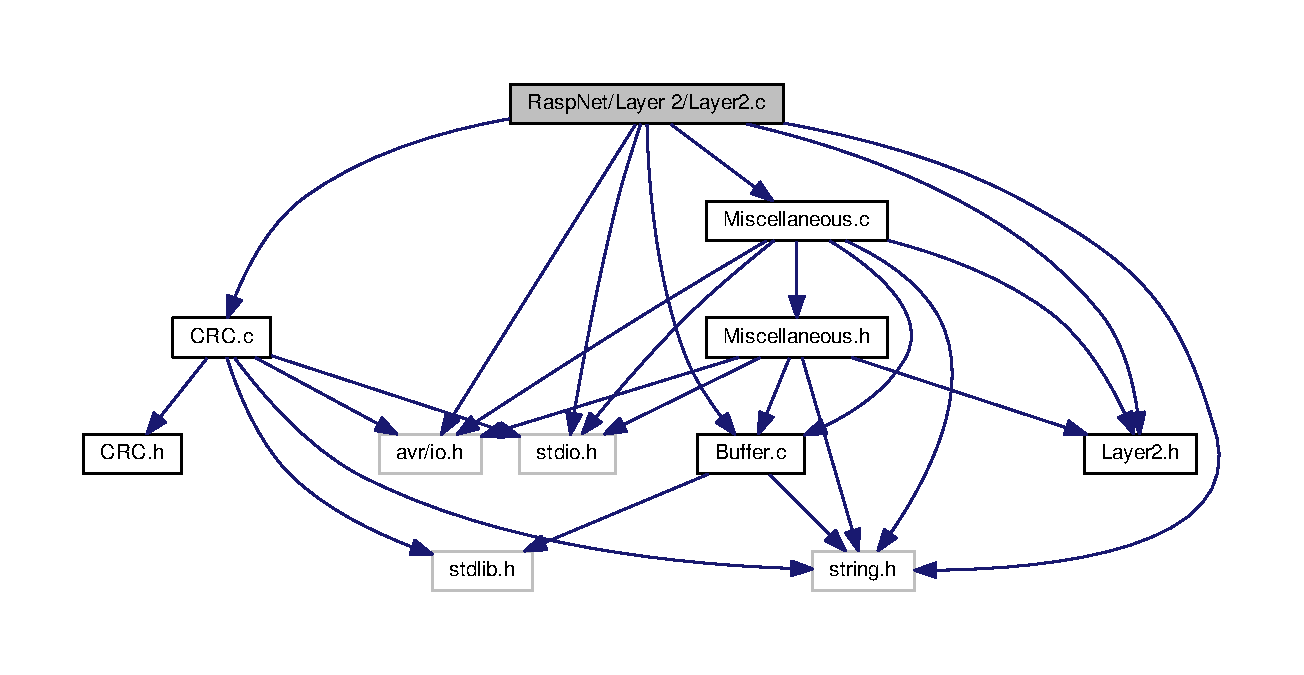
\includegraphics[width=350pt]{Layer2_8c__incl}
\end{center}
\end{figure}
This graph shows which files directly or indirectly include this file\+:
\nopagebreak
\begin{figure}[H]
\begin{center}
\leavevmode
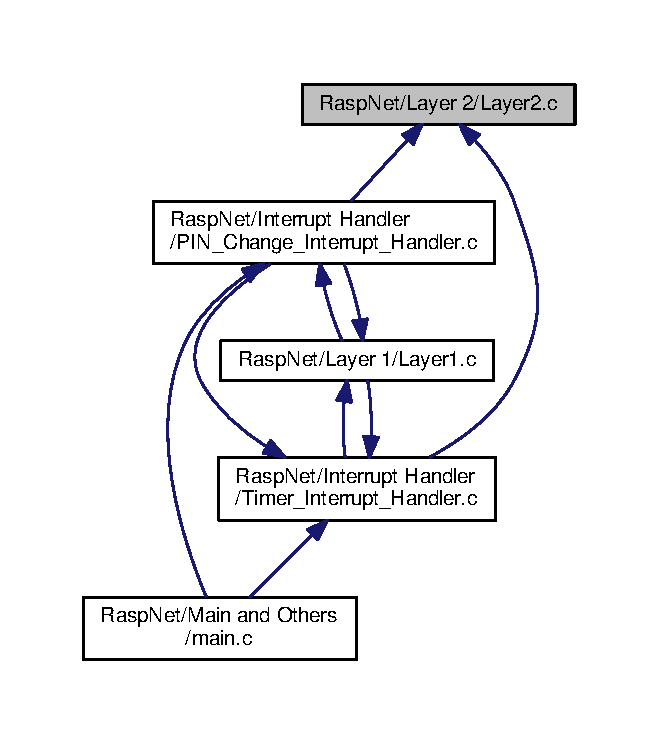
\includegraphics[width=316pt]{Layer2_8c__dep__incl}
\end{center}
\end{figure}
\subsection*{Functions}
\begin{DoxyCompactItemize}
\item 
void \hyperlink{Layer2_8c_ae785b505c564edf60c7c6a736235ddec}{tranmit\+\_\+1} ()
\begin{DoxyCompactList}\small\item\em Transmit data signal as H\+I\+GH or 1 through the data pin. \end{DoxyCompactList}\item 
void \hyperlink{Layer2_8c_ae79cf97d224edfd2ebfabc1a049360ce}{tranmit\+\_\+0} ()
\begin{DoxyCompactList}\small\item\em Transmit data signal as L\+OW or 0 through the data pin. \end{DoxyCompactList}\item 
int \hyperlink{Layer2_8c_a5c4475bf56e57eeadef01672aa670a82}{data\+\_\+receive} ()
\begin{DoxyCompactList}\small\item\em Read the status of the receiver data pin. \end{DoxyCompactList}\end{DoxyCompactItemize}


\subsection{Function Documentation}
\index{Layer2.\+c@{Layer2.\+c}!data\+\_\+receive@{data\+\_\+receive}}
\index{data\+\_\+receive@{data\+\_\+receive}!Layer2.\+c@{Layer2.\+c}}
\subsubsection[{\texorpdfstring{data\+\_\+receive()}{data_receive()}}]{\setlength{\rightskip}{0pt plus 5cm}int data\+\_\+receive (
\begin{DoxyParamCaption}
{}
\end{DoxyParamCaption}
)}\hypertarget{Layer2_8c_a5c4475bf56e57eeadef01672aa670a82}{}\label{Layer2_8c_a5c4475bf56e57eeadef01672aa670a82}


Read the status of the receiver data pin. 

\begin{DoxyReturn}{Returns}
integer data which are 0 or 1 
\end{DoxyReturn}
$<$ Receiver read the status of P\+D5 pin

$<$ When P\+D5 is H\+I\+GH return 1

$<$ When P\+D5 is L\+OW return 0 
\begin{DoxyCode}
24                    \{
25     \textcolor{keywordflow}{if}(PIND&(1<<PD5)) \{ 
26         \textcolor{keywordflow}{return} 1;   
27     \}
28     \textcolor{keywordflow}{else} \{
29         \textcolor{keywordflow}{return} 0; 
30     \}
31 \}
\end{DoxyCode}
\index{Layer2.\+c@{Layer2.\+c}!tranmit\+\_\+0@{tranmit\+\_\+0}}
\index{tranmit\+\_\+0@{tranmit\+\_\+0}!Layer2.\+c@{Layer2.\+c}}
\subsubsection[{\texorpdfstring{tranmit\+\_\+0()}{tranmit_0()}}]{\setlength{\rightskip}{0pt plus 5cm}void tranmit\+\_\+0 (
\begin{DoxyParamCaption}
{}
\end{DoxyParamCaption}
)}\hypertarget{Layer2_8c_ae79cf97d224edfd2ebfabc1a049360ce}{}\label{Layer2_8c_ae79cf97d224edfd2ebfabc1a049360ce}


Transmit data signal as L\+OW or 0 through the data pin. 

\begin{DoxyReturn}{Returns}
void nothing has to be returned 
\end{DoxyReturn}
$<$ Make P\+B5 pin L\+OW for data transmit 
\begin{DoxyCode}
17                  \{
18 
19     PORTB&=~(1<<PB5); 
20 \}
\end{DoxyCode}
\index{Layer2.\+c@{Layer2.\+c}!tranmit\+\_\+1@{tranmit\+\_\+1}}
\index{tranmit\+\_\+1@{tranmit\+\_\+1}!Layer2.\+c@{Layer2.\+c}}
\subsubsection[{\texorpdfstring{tranmit\+\_\+1()}{tranmit_1()}}]{\setlength{\rightskip}{0pt plus 5cm}void tranmit\+\_\+1 (
\begin{DoxyParamCaption}
{}
\end{DoxyParamCaption}
)}\hypertarget{Layer2_8c_ae785b505c564edf60c7c6a736235ddec}{}\label{Layer2_8c_ae785b505c564edf60c7c6a736235ddec}


Transmit data signal as H\+I\+GH or 1 through the data pin. 

\begin{DoxyReturn}{Returns}
void nothing has to be returned 
\end{DoxyReturn}
$<$ Make P\+B5 pin H\+I\+GH for data transmit 
\begin{DoxyCode}
11                  \{
12 
13     PORTB|=(1<<PB5); 
15 \}
\end{DoxyCode}

\hypertarget{Layer2_8h}{}\section{Rasp\+Net/\+Layer 2/\+Layer2.h File Reference}
\label{Layer2_8h}\index{Rasp\+Net/\+Layer 2/\+Layer2.\+h@{Rasp\+Net/\+Layer 2/\+Layer2.\+h}}
This graph shows which files directly or indirectly include this file\+:
\nopagebreak
\begin{figure}[H]
\begin{center}
\leavevmode
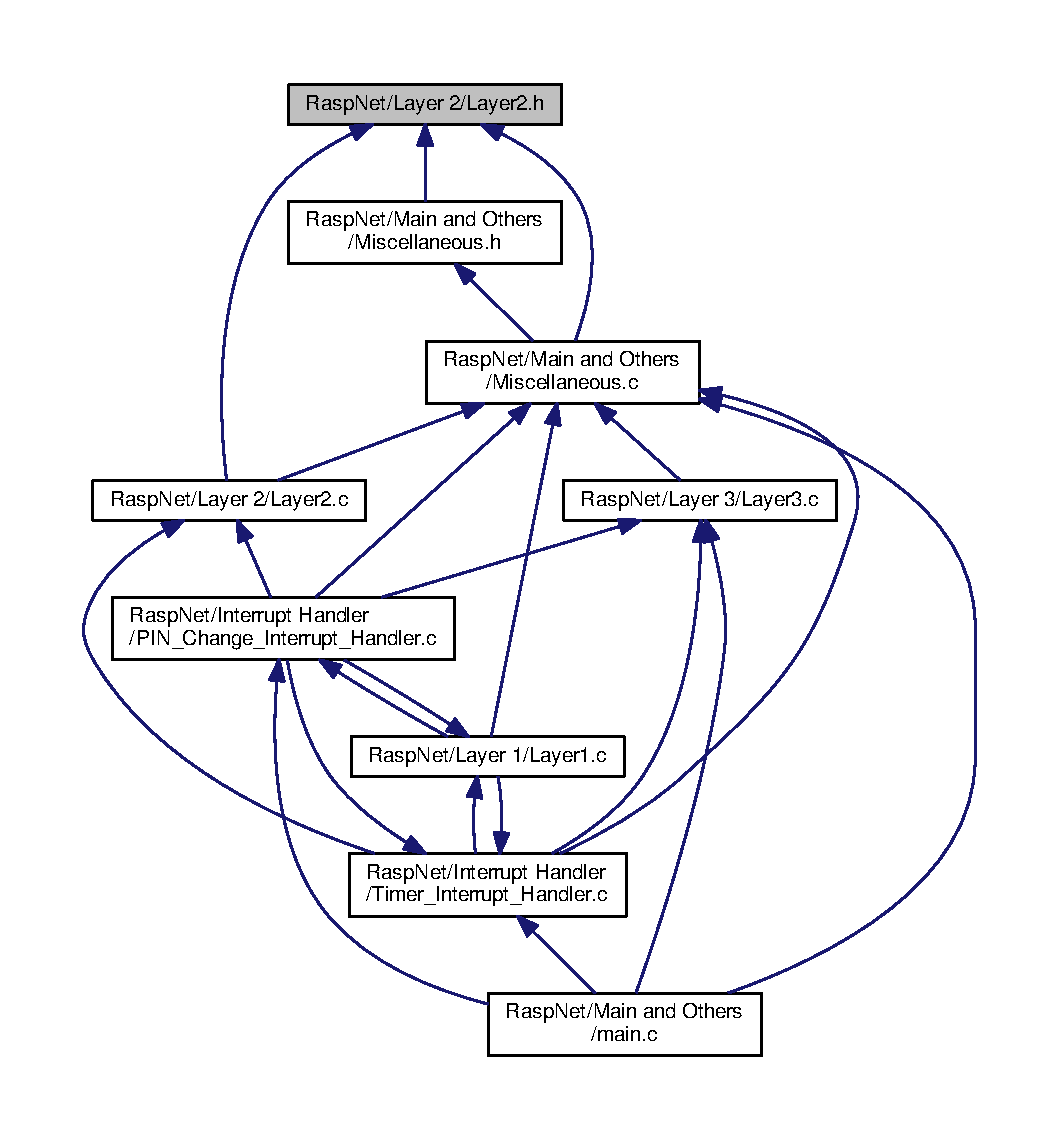
\includegraphics[width=350pt]{Layer2_8h__dep__incl}
\end{center}
\end{figure}
\subsection*{Functions}
\begin{DoxyCompactItemize}
\item 
int \hyperlink{Layer2_8h_a5c4475bf56e57eeadef01672aa670a82}{data\+\_\+receive} ()
\begin{DoxyCompactList}\small\item\em Read the status of the receiver data pin. \end{DoxyCompactList}\item 
void \hyperlink{Layer2_8h_ae785b505c564edf60c7c6a736235ddec}{tranmit\+\_\+1} ()
\begin{DoxyCompactList}\small\item\em Transmit data signal as H\+I\+GH or 1 through the data pin. \end{DoxyCompactList}\item 
void \hyperlink{Layer2_8h_ae79cf97d224edfd2ebfabc1a049360ce}{tranmit\+\_\+0} ()
\begin{DoxyCompactList}\small\item\em Transmit data signal as L\+OW or 0 through the data pin. \end{DoxyCompactList}\end{DoxyCompactItemize}


\subsection{Function Documentation}
\index{Layer2.\+h@{Layer2.\+h}!data\+\_\+receive@{data\+\_\+receive}}
\index{data\+\_\+receive@{data\+\_\+receive}!Layer2.\+h@{Layer2.\+h}}
\subsubsection[{\texorpdfstring{data\+\_\+receive()}{data_receive()}}]{\setlength{\rightskip}{0pt plus 5cm}int data\+\_\+receive (
\begin{DoxyParamCaption}
{}
\end{DoxyParamCaption}
)}\hypertarget{Layer2_8h_a5c4475bf56e57eeadef01672aa670a82}{}\label{Layer2_8h_a5c4475bf56e57eeadef01672aa670a82}


Read the status of the receiver data pin. 

\begin{DoxyReturn}{Returns}
integer data which are 0 or 1 
\end{DoxyReturn}
$<$ Receiver read the status of P\+D5 pin

$<$ When P\+D5 is H\+I\+GH return 1

$<$ When P\+D5 is L\+OW return 0 
\begin{DoxyCode}
24                    \{
25     \textcolor{keywordflow}{if}(PIND&(1<<PD5)) \{ 
26         \textcolor{keywordflow}{return} 1;   
27     \}
28     \textcolor{keywordflow}{else} \{
29         \textcolor{keywordflow}{return} 0; 
30     \}
31 \}
\end{DoxyCode}
\index{Layer2.\+h@{Layer2.\+h}!tranmit\+\_\+0@{tranmit\+\_\+0}}
\index{tranmit\+\_\+0@{tranmit\+\_\+0}!Layer2.\+h@{Layer2.\+h}}
\subsubsection[{\texorpdfstring{tranmit\+\_\+0()}{tranmit_0()}}]{\setlength{\rightskip}{0pt plus 5cm}void tranmit\+\_\+0 (
\begin{DoxyParamCaption}
{}
\end{DoxyParamCaption}
)}\hypertarget{Layer2_8h_ae79cf97d224edfd2ebfabc1a049360ce}{}\label{Layer2_8h_ae79cf97d224edfd2ebfabc1a049360ce}


Transmit data signal as L\+OW or 0 through the data pin. 

\begin{DoxyReturn}{Returns}
void nothing has to be returned 
\end{DoxyReturn}
$<$ Make P\+B5 pin L\+OW for data transmit 
\begin{DoxyCode}
17                  \{
18 
19     PORTB&=~(1<<PB5); 
20 \}
\end{DoxyCode}
\index{Layer2.\+h@{Layer2.\+h}!tranmit\+\_\+1@{tranmit\+\_\+1}}
\index{tranmit\+\_\+1@{tranmit\+\_\+1}!Layer2.\+h@{Layer2.\+h}}
\subsubsection[{\texorpdfstring{tranmit\+\_\+1()}{tranmit_1()}}]{\setlength{\rightskip}{0pt plus 5cm}void tranmit\+\_\+1 (
\begin{DoxyParamCaption}
{}
\end{DoxyParamCaption}
)}\hypertarget{Layer2_8h_ae785b505c564edf60c7c6a736235ddec}{}\label{Layer2_8h_ae785b505c564edf60c7c6a736235ddec}


Transmit data signal as H\+I\+GH or 1 through the data pin. 

\begin{DoxyReturn}{Returns}
void nothing has to be returned 
\end{DoxyReturn}
$<$ Make P\+B5 pin H\+I\+GH for data transmit 
\begin{DoxyCode}
11                  \{
12 
13     PORTB|=(1<<PB5); 
15 \}
\end{DoxyCode}

\hypertarget{Layer3_8c}{}\section{Rasp\+Net/\+Layer 3/\+Layer3.c File Reference}
\label{Layer3_8c}\index{Rasp\+Net/\+Layer 3/\+Layer3.\+c@{Rasp\+Net/\+Layer 3/\+Layer3.\+c}}
{\ttfamily \#include \char`\"{}Layer3.\+h\char`\"{}}\\*
{\ttfamily \#include \char`\"{}Miscellaneous.\+c\char`\"{}}\\*
Include dependency graph for Layer3.\+c\+:
\nopagebreak
\begin{figure}[H]
\begin{center}
\leavevmode
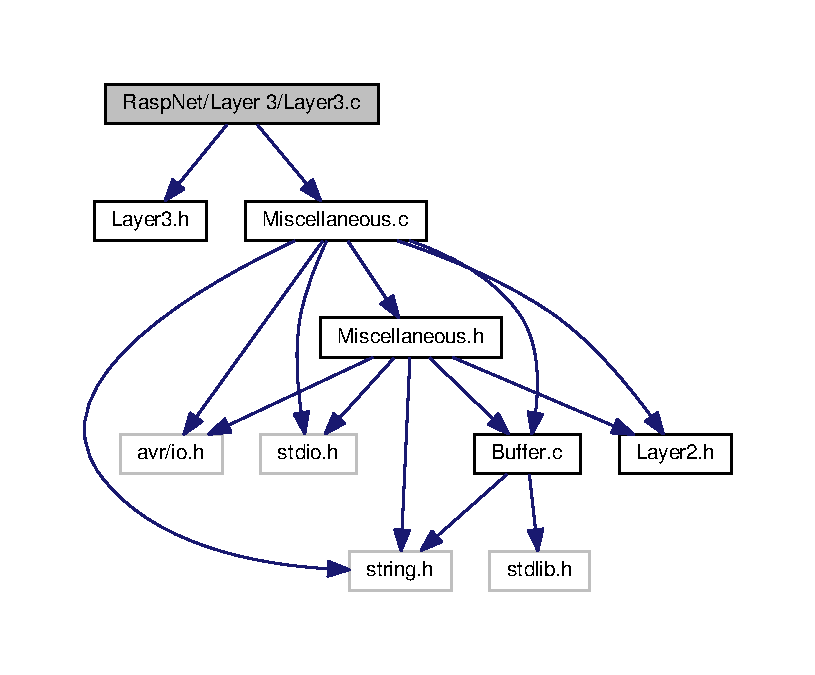
\includegraphics[width=350pt]{Layer3_8c__incl}
\end{center}
\end{figure}
This graph shows which files directly or indirectly include this file\+:
\nopagebreak
\begin{figure}[H]
\begin{center}
\leavevmode
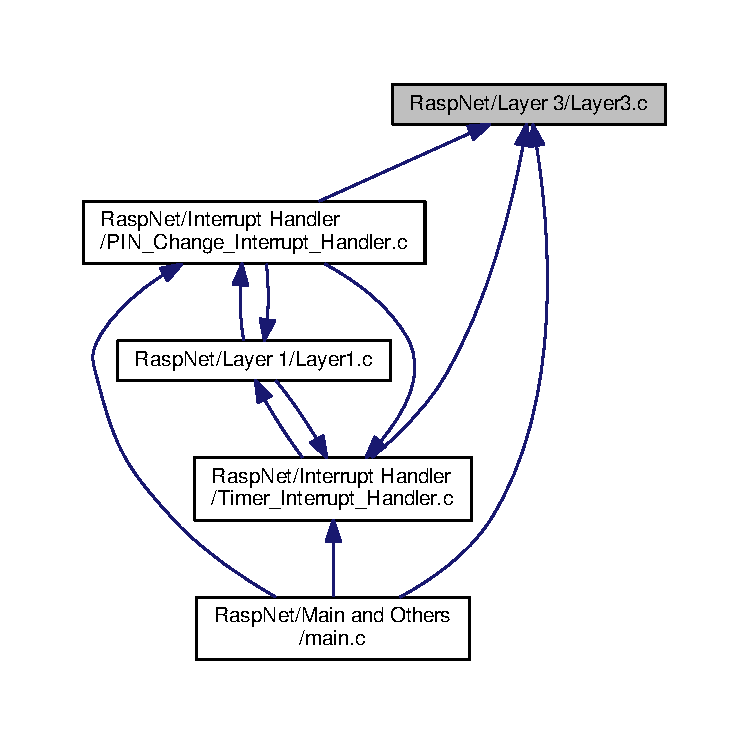
\includegraphics[width=350pt]{Layer3_8c__dep__incl}
\end{center}
\end{figure}
\subsection*{Functions}
\begin{DoxyCompactItemize}
\item 
void \hyperlink{Layer3_8c_a5cc35a45674625cd8733379d3f0523b8}{discard\+\_\+packet} (struct \hyperlink{structPacket}{Packet} $\ast$packet)
\begin{DoxyCompactList}\small\item\em This function is used to delete packet. \end{DoxyCompactList}\item 
int \hyperlink{Layer3_8c_a23b38c7493fb43e33264c3972782f496}{type\+\_\+of\+\_\+msg} (struct \hyperlink{structPacket}{Packet} $\ast$packet)
\begin{DoxyCompactList}\small\item\em This function is used to detect the type of message. \end{DoxyCompactList}\end{DoxyCompactItemize}


\subsection{Function Documentation}
\index{Layer3.\+c@{Layer3.\+c}!discard\+\_\+packet@{discard\+\_\+packet}}
\index{discard\+\_\+packet@{discard\+\_\+packet}!Layer3.\+c@{Layer3.\+c}}
\subsubsection[{\texorpdfstring{discard\+\_\+packet(struct Packet $\ast$packet)}{discard_packet(struct Packet *packet)}}]{\setlength{\rightskip}{0pt plus 5cm}void discard\+\_\+packet (
\begin{DoxyParamCaption}
\item[{struct {\bf Packet} $\ast$}]{packet}
\end{DoxyParamCaption}
)}\hypertarget{Layer3_8c_a5cc35a45674625cd8733379d3f0523b8}{}\label{Layer3_8c_a5cc35a45674625cd8733379d3f0523b8}


This function is used to delete packet. 


\begin{DoxyParams}{Parameters}
{\em f} & structure pointer, it\textquotesingle{}s type is \hyperlink{structPacket}{Packet} \\
\hline
\end{DoxyParams}
\begin{DoxyReturn}{Returns}
void nothing has to return from this function 
\end{DoxyReturn}

\begin{DoxyCode}
5                                           \{
6     packet->\hyperlink{structPacket_af626fe07d93fe4116d613304792df080}{destination}=0;
7     packet->\hyperlink{structPacket_a01308f5b690e5060fea6037e765058b9}{source}=0b00000000;
8     packet->\hyperlink{structPacket_aa305c88136c91911a5159610863cb41d}{preamble}=0b00000000;
9     packet->\hyperlink{structPacket_ab13014675ea9eda122b1c50842a567fc}{payload\_siz}=0b00000000;
10     packet->\hyperlink{structPacket_abad95795e9615463d9d69d298a86b0b8}{crc}=0b00000000000000000000000000000000;
11 \}
\end{DoxyCode}
\index{Layer3.\+c@{Layer3.\+c}!type\+\_\+of\+\_\+msg@{type\+\_\+of\+\_\+msg}}
\index{type\+\_\+of\+\_\+msg@{type\+\_\+of\+\_\+msg}!Layer3.\+c@{Layer3.\+c}}
\subsubsection[{\texorpdfstring{type\+\_\+of\+\_\+msg(struct Packet $\ast$packet)}{type_of_msg(struct Packet *packet)}}]{\setlength{\rightskip}{0pt plus 5cm}int type\+\_\+of\+\_\+msg (
\begin{DoxyParamCaption}
\item[{struct {\bf Packet} $\ast$}]{packet}
\end{DoxyParamCaption}
)}\hypertarget{Layer3_8c_a23b38c7493fb43e33264c3972782f496}{}\label{Layer3_8c_a23b38c7493fb43e33264c3972782f496}


This function is used to detect the type of message. 


\begin{DoxyParams}{Parameters}
{\em f} & structure pointer, it\textquotesingle{}s type is \hyperlink{structPacket}{Packet} \\
\hline
\end{DoxyParams}
\begin{DoxyReturn}{Returns}
integer type data, which is defined in macro 
\end{DoxyReturn}
$<$ At first initiaze message type as unknown

$<$ Extract the source address

$<$ Extract destination address

$<$Return my own message to me

$<$Receive my own broadcasting message

$<$ Receive broadcasting message

$<$ Message send to me

$<$Message send to other node\+: relay

$<$Message from unknown source which can not be identified 
\begin{DoxyCode}
14                                       \{
15     \textcolor{keywordtype}{int} message\_type=\hyperlink{Layer3_8h_a09741204cd73a0942c6f97dd0e9d3108}{unknown}; 
16     \textcolor{keywordtype}{int} source\_address = packet->\hyperlink{structPacket_a01308f5b690e5060fea6037e765058b9}{source}; 
17     \textcolor{keywordtype}{int} destination\_address=packet->\hyperlink{structPacket_af626fe07d93fe4116d613304792df080}{destination}; 
19     \textcolor{keywordflow}{if}((source\_address==\hyperlink{Layer3_8h_aeb49fa593cb6818cfc97aee412e3eb8d}{my\_own\_id}) && (destination\_address!=
      \hyperlink{Layer3_8h_aab720f22f66cc3daa0e843089e24d628}{broadcasting\_id}))\{
20         message\_type=\hyperlink{Layer3_8h_ab7153c7289145c9aab31e838d3f29b0f}{return\_my\_own\_msg}; 
22     \}
23     \textcolor{keywordflow}{else} \textcolor{keywordflow}{if}((source\_address==\hyperlink{Layer3_8h_aeb49fa593cb6818cfc97aee412e3eb8d}{my\_own\_id}) && (destination\_address==
      \hyperlink{Layer3_8h_aab720f22f66cc3daa0e843089e24d628}{broadcasting\_id}))\{
24         message\_type=\hyperlink{Layer3_8h_a58352e6aa962709f6a002dbc21406113}{my\_own\_braodcasting\_msg}; 
25     \}
26 
27 
28     \textcolor{keywordflow}{else} \textcolor{keywordflow}{if}((!(source\_address==\hyperlink{Layer3_8h_aeb49fa593cb6818cfc97aee412e3eb8d}{my\_own\_id})) && (destination\_address==
      \hyperlink{Layer3_8h_aab720f22f66cc3daa0e843089e24d628}{broadcasting\_id}))\{
29         message\_type=\hyperlink{Layer3_8h_a3bd3ae1527491d97c67f22e569f296a4}{broadcasting\_msg}; 
30     \}
31 
32     \textcolor{keywordflow}{else} \textcolor{keywordflow}{if}((!(source\_address==\hyperlink{Layer3_8h_aeb49fa593cb6818cfc97aee412e3eb8d}{my\_own\_id})) && (destination\_address==
      \hyperlink{Layer3_8h_aeb49fa593cb6818cfc97aee412e3eb8d}{my\_own\_id}))\{
33         message\_type=\hyperlink{Layer3_8h_a465792308892364b6fd0d58cf45b6043}{msg\_send\_to\_me}; 
34     \}
35     \textcolor{keywordflow}{else} \textcolor{keywordflow}{if}((!(source\_address==\hyperlink{Layer3_8h_aeb49fa593cb6818cfc97aee412e3eb8d}{my\_own\_id})) && (!(destination\_address==
      \hyperlink{Layer3_8h_aeb49fa593cb6818cfc97aee412e3eb8d}{my\_own\_id})) &&
36         (!(destination\_address==\hyperlink{Layer3_8h_a3bd3ae1527491d97c67f22e569f296a4}{broadcasting\_msg})))\{
37         message\_type=\hyperlink{Layer3_8h_a8aa9037a9afe926a10f769adc957936a}{msg\_send\_to\_other\_node}; 
38     \}
39 
40     \textcolor{keywordflow}{else}\{
41         message\_type=\hyperlink{Layer3_8h_a09741204cd73a0942c6f97dd0e9d3108}{unknown}; 
42     \}
43 
44     \textcolor{keywordflow}{return} message\_type;
45 
46 \}
\end{DoxyCode}

\hypertarget{Layer3_8h}{}\section{Rasp\+Net/\+Layer 3/\+Layer3.h File Reference}
\label{Layer3_8h}\index{Rasp\+Net/\+Layer 3/\+Layer3.\+h@{Rasp\+Net/\+Layer 3/\+Layer3.\+h}}
This graph shows which files directly or indirectly include this file\+:
\nopagebreak
\begin{figure}[H]
\begin{center}
\leavevmode
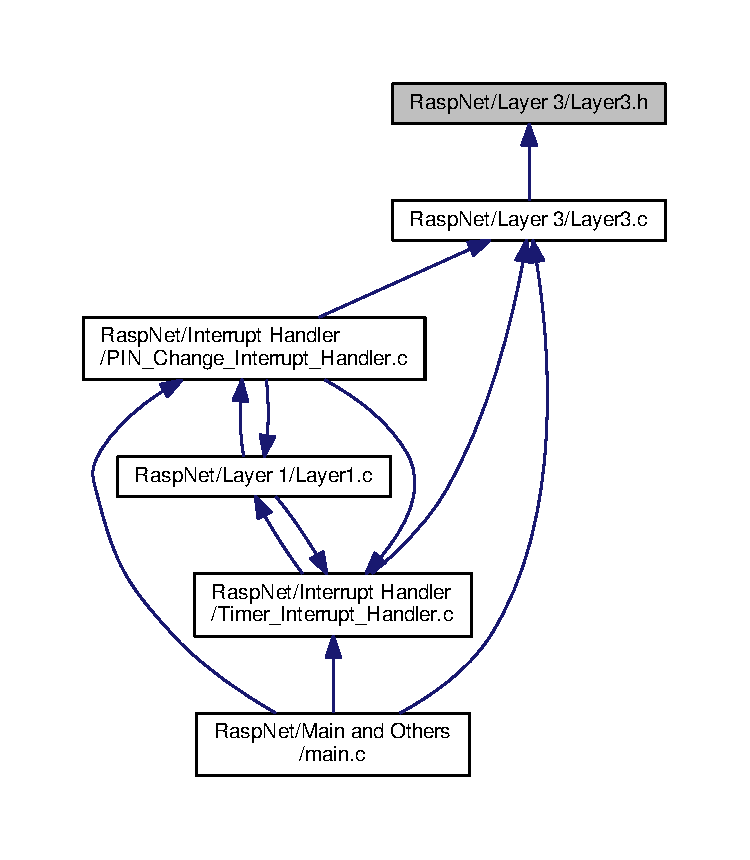
\includegraphics[width=350pt]{Layer3_8h__dep__incl}
\end{center}
\end{figure}
\subsection*{Macros}
\begin{DoxyCompactItemize}
\item 
\#define \hyperlink{Layer3_8h_aeb49fa593cb6818cfc97aee412e3eb8d}{my\+\_\+own\+\_\+id}~1
\item 
\#define \hyperlink{Layer3_8h_aab720f22f66cc3daa0e843089e24d628}{broadcasting\+\_\+id}~0
\item 
\#define \hyperlink{Layer3_8h_afd5191a3ada0a4968402449c806bd4b3}{priority\+\_\+normal}~21
\item 
\#define \hyperlink{Layer3_8h_aaccf0a951ca84ac3578fa3bcfbac5522}{priority\+\_\+for\+\_\+relay}~22
\item 
\#define \hyperlink{Layer3_8h_a3b7ed14628679beda488dc3269b7b6a0}{priority\+\_\+for\+\_\+sending\+\_\+order}~23
\item 
\#define \hyperlink{Layer3_8h_a4a793a607f3e830119fe598d76630898}{priority\+\_\+high}~24
\item 
\#define \hyperlink{Layer3_8h_ab7153c7289145c9aab31e838d3f29b0f}{return\+\_\+my\+\_\+own\+\_\+msg}~101
\item 
\#define \hyperlink{Layer3_8h_a58352e6aa962709f6a002dbc21406113}{my\+\_\+own\+\_\+braodcasting\+\_\+msg}~102
\item 
\#define \hyperlink{Layer3_8h_a3bd3ae1527491d97c67f22e569f296a4}{broadcasting\+\_\+msg}~103
\item 
\#define \hyperlink{Layer3_8h_a465792308892364b6fd0d58cf45b6043}{msg\+\_\+send\+\_\+to\+\_\+me}~104
\item 
\#define \hyperlink{Layer3_8h_a8aa9037a9afe926a10f769adc957936a}{msg\+\_\+send\+\_\+to\+\_\+other\+\_\+node}~105
\item 
\#define \hyperlink{Layer3_8h_a09741204cd73a0942c6f97dd0e9d3108}{unknown}~-\/111
\item 
\#define \hyperlink{Layer3_8h_a5b4f913d88d52723f970056a0ea4dd09}{transmit\+\_\+preamble}~31
\item 
\#define \hyperlink{Layer3_8h_a44e78cb310dd2d291b3d3f96c2a4fbf3}{transmit\+\_\+destination\+\_\+address}~32
\item 
\#define \hyperlink{Layer3_8h_aa4e2ceb5bd48f2fde7e6c7240ca66e44}{transmit\+\_\+source\+\_\+address}~33
\item 
\#define \hyperlink{Layer3_8h_a97826fb6e7415b7cca5b6f704b2c37fc}{transmit\+\_\+crc}~34
\item 
\#define \hyperlink{Layer3_8h_a6b4b30550290df6d0f6c7726714672bf}{transmit\+\_\+payload\+\_\+size}~35
\item 
\#define \hyperlink{Layer3_8h_afde148ebf464f31e83576556e5bc4102}{transmit\+\_\+payload}~36
\item 
\#define \hyperlink{Layer3_8h_af43b7652801ee9e083162514d5372e9f}{transmitted}~37
\item 
\#define \hyperlink{Layer3_8h_aa8ef63ae0468c77b8312b92d7154609d}{receive\+\_\+preamble}~41
\item 
\#define \hyperlink{Layer3_8h_a39e1380303eff462d17201a4cd077b31}{receive\+\_\+destination\+\_\+address}~42
\item 
\#define \hyperlink{Layer3_8h_ace2bdbcd80ee617b80126b378b51dfe3}{receive\+\_\+source\+\_\+address}~43
\item 
\#define \hyperlink{Layer3_8h_aa59256b98f189dbcee223214dfde1c49}{receive\+\_\+crc}~44
\item 
\#define \hyperlink{Layer3_8h_a1c9fabd7b0478766bb4b611e5dbe8853}{receive\+\_\+payload\+\_\+size}~45
\item 
\#define \hyperlink{Layer3_8h_a8fc3575b730c4bc458cdce87537175d1}{receive\+\_\+payload}~46
\item 
\#define \hyperlink{Layer3_8h_ae248a94ed37c2d8dad80d8a627ad9974}{received\+\_\+crc\+\_\+check}~47
\end{DoxyCompactItemize}
\subsection*{Functions}
\begin{DoxyCompactItemize}
\item 
void \hyperlink{Layer3_8h_a5cc35a45674625cd8733379d3f0523b8}{discard\+\_\+packet} (struct \hyperlink{structPacket}{Packet} $\ast$packet)
\begin{DoxyCompactList}\small\item\em This function is used to delete packet. \end{DoxyCompactList}\item 
int \hyperlink{Layer3_8h_a23b38c7493fb43e33264c3972782f496}{type\+\_\+of\+\_\+msg} (struct \hyperlink{structPacket}{Packet} $\ast$packet)
\begin{DoxyCompactList}\small\item\em This function is used to detect the type of message. \end{DoxyCompactList}\end{DoxyCompactItemize}
\subsection*{Variables}
\begin{DoxyCompactItemize}
\item 
int \hyperlink{Layer3_8h_a2a0eb18d69ebbaf44dd4e863fa4f6a59}{priority\+\_\+type}
\end{DoxyCompactItemize}


\subsection{Macro Definition Documentation}
\index{Layer3.\+h@{Layer3.\+h}!broadcasting\+\_\+id@{broadcasting\+\_\+id}}
\index{broadcasting\+\_\+id@{broadcasting\+\_\+id}!Layer3.\+h@{Layer3.\+h}}
\subsubsection[{\texorpdfstring{broadcasting\+\_\+id}{broadcasting_id}}]{\setlength{\rightskip}{0pt plus 5cm}\#define broadcasting\+\_\+id~0}\hypertarget{Layer3_8h_aab720f22f66cc3daa0e843089e24d628}{}\label{Layer3_8h_aab720f22f66cc3daa0e843089e24d628}
\index{Layer3.\+h@{Layer3.\+h}!broadcasting\+\_\+msg@{broadcasting\+\_\+msg}}
\index{broadcasting\+\_\+msg@{broadcasting\+\_\+msg}!Layer3.\+h@{Layer3.\+h}}
\subsubsection[{\texorpdfstring{broadcasting\+\_\+msg}{broadcasting_msg}}]{\setlength{\rightskip}{0pt plus 5cm}\#define broadcasting\+\_\+msg~103}\hypertarget{Layer3_8h_a3bd3ae1527491d97c67f22e569f296a4}{}\label{Layer3_8h_a3bd3ae1527491d97c67f22e569f296a4}
\index{Layer3.\+h@{Layer3.\+h}!msg\+\_\+send\+\_\+to\+\_\+me@{msg\+\_\+send\+\_\+to\+\_\+me}}
\index{msg\+\_\+send\+\_\+to\+\_\+me@{msg\+\_\+send\+\_\+to\+\_\+me}!Layer3.\+h@{Layer3.\+h}}
\subsubsection[{\texorpdfstring{msg\+\_\+send\+\_\+to\+\_\+me}{msg_send_to_me}}]{\setlength{\rightskip}{0pt plus 5cm}\#define msg\+\_\+send\+\_\+to\+\_\+me~104}\hypertarget{Layer3_8h_a465792308892364b6fd0d58cf45b6043}{}\label{Layer3_8h_a465792308892364b6fd0d58cf45b6043}
\index{Layer3.\+h@{Layer3.\+h}!msg\+\_\+send\+\_\+to\+\_\+other\+\_\+node@{msg\+\_\+send\+\_\+to\+\_\+other\+\_\+node}}
\index{msg\+\_\+send\+\_\+to\+\_\+other\+\_\+node@{msg\+\_\+send\+\_\+to\+\_\+other\+\_\+node}!Layer3.\+h@{Layer3.\+h}}
\subsubsection[{\texorpdfstring{msg\+\_\+send\+\_\+to\+\_\+other\+\_\+node}{msg_send_to_other_node}}]{\setlength{\rightskip}{0pt plus 5cm}\#define msg\+\_\+send\+\_\+to\+\_\+other\+\_\+node~105}\hypertarget{Layer3_8h_a8aa9037a9afe926a10f769adc957936a}{}\label{Layer3_8h_a8aa9037a9afe926a10f769adc957936a}
\index{Layer3.\+h@{Layer3.\+h}!my\+\_\+own\+\_\+braodcasting\+\_\+msg@{my\+\_\+own\+\_\+braodcasting\+\_\+msg}}
\index{my\+\_\+own\+\_\+braodcasting\+\_\+msg@{my\+\_\+own\+\_\+braodcasting\+\_\+msg}!Layer3.\+h@{Layer3.\+h}}
\subsubsection[{\texorpdfstring{my\+\_\+own\+\_\+braodcasting\+\_\+msg}{my_own_braodcasting_msg}}]{\setlength{\rightskip}{0pt plus 5cm}\#define my\+\_\+own\+\_\+braodcasting\+\_\+msg~102}\hypertarget{Layer3_8h_a58352e6aa962709f6a002dbc21406113}{}\label{Layer3_8h_a58352e6aa962709f6a002dbc21406113}
\index{Layer3.\+h@{Layer3.\+h}!my\+\_\+own\+\_\+id@{my\+\_\+own\+\_\+id}}
\index{my\+\_\+own\+\_\+id@{my\+\_\+own\+\_\+id}!Layer3.\+h@{Layer3.\+h}}
\subsubsection[{\texorpdfstring{my\+\_\+own\+\_\+id}{my_own_id}}]{\setlength{\rightskip}{0pt plus 5cm}\#define my\+\_\+own\+\_\+id~1}\hypertarget{Layer3_8h_aeb49fa593cb6818cfc97aee412e3eb8d}{}\label{Layer3_8h_aeb49fa593cb6818cfc97aee412e3eb8d}
\index{Layer3.\+h@{Layer3.\+h}!priority\+\_\+for\+\_\+relay@{priority\+\_\+for\+\_\+relay}}
\index{priority\+\_\+for\+\_\+relay@{priority\+\_\+for\+\_\+relay}!Layer3.\+h@{Layer3.\+h}}
\subsubsection[{\texorpdfstring{priority\+\_\+for\+\_\+relay}{priority_for_relay}}]{\setlength{\rightskip}{0pt plus 5cm}\#define priority\+\_\+for\+\_\+relay~22}\hypertarget{Layer3_8h_aaccf0a951ca84ac3578fa3bcfbac5522}{}\label{Layer3_8h_aaccf0a951ca84ac3578fa3bcfbac5522}
\index{Layer3.\+h@{Layer3.\+h}!priority\+\_\+for\+\_\+sending\+\_\+order@{priority\+\_\+for\+\_\+sending\+\_\+order}}
\index{priority\+\_\+for\+\_\+sending\+\_\+order@{priority\+\_\+for\+\_\+sending\+\_\+order}!Layer3.\+h@{Layer3.\+h}}
\subsubsection[{\texorpdfstring{priority\+\_\+for\+\_\+sending\+\_\+order}{priority_for_sending_order}}]{\setlength{\rightskip}{0pt plus 5cm}\#define priority\+\_\+for\+\_\+sending\+\_\+order~23}\hypertarget{Layer3_8h_a3b7ed14628679beda488dc3269b7b6a0}{}\label{Layer3_8h_a3b7ed14628679beda488dc3269b7b6a0}
\index{Layer3.\+h@{Layer3.\+h}!priority\+\_\+high@{priority\+\_\+high}}
\index{priority\+\_\+high@{priority\+\_\+high}!Layer3.\+h@{Layer3.\+h}}
\subsubsection[{\texorpdfstring{priority\+\_\+high}{priority_high}}]{\setlength{\rightskip}{0pt plus 5cm}\#define priority\+\_\+high~24}\hypertarget{Layer3_8h_a4a793a607f3e830119fe598d76630898}{}\label{Layer3_8h_a4a793a607f3e830119fe598d76630898}
\index{Layer3.\+h@{Layer3.\+h}!priority\+\_\+normal@{priority\+\_\+normal}}
\index{priority\+\_\+normal@{priority\+\_\+normal}!Layer3.\+h@{Layer3.\+h}}
\subsubsection[{\texorpdfstring{priority\+\_\+normal}{priority_normal}}]{\setlength{\rightskip}{0pt plus 5cm}\#define priority\+\_\+normal~21}\hypertarget{Layer3_8h_afd5191a3ada0a4968402449c806bd4b3}{}\label{Layer3_8h_afd5191a3ada0a4968402449c806bd4b3}
\index{Layer3.\+h@{Layer3.\+h}!receive\+\_\+crc@{receive\+\_\+crc}}
\index{receive\+\_\+crc@{receive\+\_\+crc}!Layer3.\+h@{Layer3.\+h}}
\subsubsection[{\texorpdfstring{receive\+\_\+crc}{receive_crc}}]{\setlength{\rightskip}{0pt plus 5cm}\#define receive\+\_\+crc~44}\hypertarget{Layer3_8h_aa59256b98f189dbcee223214dfde1c49}{}\label{Layer3_8h_aa59256b98f189dbcee223214dfde1c49}
\index{Layer3.\+h@{Layer3.\+h}!receive\+\_\+destination\+\_\+address@{receive\+\_\+destination\+\_\+address}}
\index{receive\+\_\+destination\+\_\+address@{receive\+\_\+destination\+\_\+address}!Layer3.\+h@{Layer3.\+h}}
\subsubsection[{\texorpdfstring{receive\+\_\+destination\+\_\+address}{receive_destination_address}}]{\setlength{\rightskip}{0pt plus 5cm}\#define receive\+\_\+destination\+\_\+address~42}\hypertarget{Layer3_8h_a39e1380303eff462d17201a4cd077b31}{}\label{Layer3_8h_a39e1380303eff462d17201a4cd077b31}
\index{Layer3.\+h@{Layer3.\+h}!receive\+\_\+payload@{receive\+\_\+payload}}
\index{receive\+\_\+payload@{receive\+\_\+payload}!Layer3.\+h@{Layer3.\+h}}
\subsubsection[{\texorpdfstring{receive\+\_\+payload}{receive_payload}}]{\setlength{\rightskip}{0pt plus 5cm}\#define receive\+\_\+payload~46}\hypertarget{Layer3_8h_a8fc3575b730c4bc458cdce87537175d1}{}\label{Layer3_8h_a8fc3575b730c4bc458cdce87537175d1}
\index{Layer3.\+h@{Layer3.\+h}!receive\+\_\+payload\+\_\+size@{receive\+\_\+payload\+\_\+size}}
\index{receive\+\_\+payload\+\_\+size@{receive\+\_\+payload\+\_\+size}!Layer3.\+h@{Layer3.\+h}}
\subsubsection[{\texorpdfstring{receive\+\_\+payload\+\_\+size}{receive_payload_size}}]{\setlength{\rightskip}{0pt plus 5cm}\#define receive\+\_\+payload\+\_\+size~45}\hypertarget{Layer3_8h_a1c9fabd7b0478766bb4b611e5dbe8853}{}\label{Layer3_8h_a1c9fabd7b0478766bb4b611e5dbe8853}
\index{Layer3.\+h@{Layer3.\+h}!receive\+\_\+preamble@{receive\+\_\+preamble}}
\index{receive\+\_\+preamble@{receive\+\_\+preamble}!Layer3.\+h@{Layer3.\+h}}
\subsubsection[{\texorpdfstring{receive\+\_\+preamble}{receive_preamble}}]{\setlength{\rightskip}{0pt plus 5cm}\#define receive\+\_\+preamble~41}\hypertarget{Layer3_8h_aa8ef63ae0468c77b8312b92d7154609d}{}\label{Layer3_8h_aa8ef63ae0468c77b8312b92d7154609d}
\index{Layer3.\+h@{Layer3.\+h}!receive\+\_\+source\+\_\+address@{receive\+\_\+source\+\_\+address}}
\index{receive\+\_\+source\+\_\+address@{receive\+\_\+source\+\_\+address}!Layer3.\+h@{Layer3.\+h}}
\subsubsection[{\texorpdfstring{receive\+\_\+source\+\_\+address}{receive_source_address}}]{\setlength{\rightskip}{0pt plus 5cm}\#define receive\+\_\+source\+\_\+address~43}\hypertarget{Layer3_8h_ace2bdbcd80ee617b80126b378b51dfe3}{}\label{Layer3_8h_ace2bdbcd80ee617b80126b378b51dfe3}
\index{Layer3.\+h@{Layer3.\+h}!received\+\_\+crc\+\_\+check@{received\+\_\+crc\+\_\+check}}
\index{received\+\_\+crc\+\_\+check@{received\+\_\+crc\+\_\+check}!Layer3.\+h@{Layer3.\+h}}
\subsubsection[{\texorpdfstring{received\+\_\+crc\+\_\+check}{received_crc_check}}]{\setlength{\rightskip}{0pt plus 5cm}\#define received\+\_\+crc\+\_\+check~47}\hypertarget{Layer3_8h_ae248a94ed37c2d8dad80d8a627ad9974}{}\label{Layer3_8h_ae248a94ed37c2d8dad80d8a627ad9974}
\index{Layer3.\+h@{Layer3.\+h}!return\+\_\+my\+\_\+own\+\_\+msg@{return\+\_\+my\+\_\+own\+\_\+msg}}
\index{return\+\_\+my\+\_\+own\+\_\+msg@{return\+\_\+my\+\_\+own\+\_\+msg}!Layer3.\+h@{Layer3.\+h}}
\subsubsection[{\texorpdfstring{return\+\_\+my\+\_\+own\+\_\+msg}{return_my_own_msg}}]{\setlength{\rightskip}{0pt plus 5cm}\#define return\+\_\+my\+\_\+own\+\_\+msg~101}\hypertarget{Layer3_8h_ab7153c7289145c9aab31e838d3f29b0f}{}\label{Layer3_8h_ab7153c7289145c9aab31e838d3f29b0f}
\index{Layer3.\+h@{Layer3.\+h}!transmit\+\_\+crc@{transmit\+\_\+crc}}
\index{transmit\+\_\+crc@{transmit\+\_\+crc}!Layer3.\+h@{Layer3.\+h}}
\subsubsection[{\texorpdfstring{transmit\+\_\+crc}{transmit_crc}}]{\setlength{\rightskip}{0pt plus 5cm}\#define transmit\+\_\+crc~34}\hypertarget{Layer3_8h_a97826fb6e7415b7cca5b6f704b2c37fc}{}\label{Layer3_8h_a97826fb6e7415b7cca5b6f704b2c37fc}
\index{Layer3.\+h@{Layer3.\+h}!transmit\+\_\+destination\+\_\+address@{transmit\+\_\+destination\+\_\+address}}
\index{transmit\+\_\+destination\+\_\+address@{transmit\+\_\+destination\+\_\+address}!Layer3.\+h@{Layer3.\+h}}
\subsubsection[{\texorpdfstring{transmit\+\_\+destination\+\_\+address}{transmit_destination_address}}]{\setlength{\rightskip}{0pt plus 5cm}\#define transmit\+\_\+destination\+\_\+address~32}\hypertarget{Layer3_8h_a44e78cb310dd2d291b3d3f96c2a4fbf3}{}\label{Layer3_8h_a44e78cb310dd2d291b3d3f96c2a4fbf3}
\index{Layer3.\+h@{Layer3.\+h}!transmit\+\_\+payload@{transmit\+\_\+payload}}
\index{transmit\+\_\+payload@{transmit\+\_\+payload}!Layer3.\+h@{Layer3.\+h}}
\subsubsection[{\texorpdfstring{transmit\+\_\+payload}{transmit_payload}}]{\setlength{\rightskip}{0pt plus 5cm}\#define transmit\+\_\+payload~36}\hypertarget{Layer3_8h_afde148ebf464f31e83576556e5bc4102}{}\label{Layer3_8h_afde148ebf464f31e83576556e5bc4102}
\index{Layer3.\+h@{Layer3.\+h}!transmit\+\_\+payload\+\_\+size@{transmit\+\_\+payload\+\_\+size}}
\index{transmit\+\_\+payload\+\_\+size@{transmit\+\_\+payload\+\_\+size}!Layer3.\+h@{Layer3.\+h}}
\subsubsection[{\texorpdfstring{transmit\+\_\+payload\+\_\+size}{transmit_payload_size}}]{\setlength{\rightskip}{0pt plus 5cm}\#define transmit\+\_\+payload\+\_\+size~35}\hypertarget{Layer3_8h_a6b4b30550290df6d0f6c7726714672bf}{}\label{Layer3_8h_a6b4b30550290df6d0f6c7726714672bf}
\index{Layer3.\+h@{Layer3.\+h}!transmit\+\_\+preamble@{transmit\+\_\+preamble}}
\index{transmit\+\_\+preamble@{transmit\+\_\+preamble}!Layer3.\+h@{Layer3.\+h}}
\subsubsection[{\texorpdfstring{transmit\+\_\+preamble}{transmit_preamble}}]{\setlength{\rightskip}{0pt plus 5cm}\#define transmit\+\_\+preamble~31}\hypertarget{Layer3_8h_a5b4f913d88d52723f970056a0ea4dd09}{}\label{Layer3_8h_a5b4f913d88d52723f970056a0ea4dd09}
\index{Layer3.\+h@{Layer3.\+h}!transmit\+\_\+source\+\_\+address@{transmit\+\_\+source\+\_\+address}}
\index{transmit\+\_\+source\+\_\+address@{transmit\+\_\+source\+\_\+address}!Layer3.\+h@{Layer3.\+h}}
\subsubsection[{\texorpdfstring{transmit\+\_\+source\+\_\+address}{transmit_source_address}}]{\setlength{\rightskip}{0pt plus 5cm}\#define transmit\+\_\+source\+\_\+address~33}\hypertarget{Layer3_8h_aa4e2ceb5bd48f2fde7e6c7240ca66e44}{}\label{Layer3_8h_aa4e2ceb5bd48f2fde7e6c7240ca66e44}
\index{Layer3.\+h@{Layer3.\+h}!transmitted@{transmitted}}
\index{transmitted@{transmitted}!Layer3.\+h@{Layer3.\+h}}
\subsubsection[{\texorpdfstring{transmitted}{transmitted}}]{\setlength{\rightskip}{0pt plus 5cm}\#define transmitted~37}\hypertarget{Layer3_8h_af43b7652801ee9e083162514d5372e9f}{}\label{Layer3_8h_af43b7652801ee9e083162514d5372e9f}
\index{Layer3.\+h@{Layer3.\+h}!unknown@{unknown}}
\index{unknown@{unknown}!Layer3.\+h@{Layer3.\+h}}
\subsubsection[{\texorpdfstring{unknown}{unknown}}]{\setlength{\rightskip}{0pt plus 5cm}\#define unknown~-\/111}\hypertarget{Layer3_8h_a09741204cd73a0942c6f97dd0e9d3108}{}\label{Layer3_8h_a09741204cd73a0942c6f97dd0e9d3108}


\subsection{Function Documentation}
\index{Layer3.\+h@{Layer3.\+h}!discard\+\_\+packet@{discard\+\_\+packet}}
\index{discard\+\_\+packet@{discard\+\_\+packet}!Layer3.\+h@{Layer3.\+h}}
\subsubsection[{\texorpdfstring{discard\+\_\+packet(struct Packet $\ast$packet)}{discard_packet(struct Packet *packet)}}]{\setlength{\rightskip}{0pt plus 5cm}void discard\+\_\+packet (
\begin{DoxyParamCaption}
\item[{struct {\bf Packet} $\ast$}]{packet}
\end{DoxyParamCaption}
)}\hypertarget{Layer3_8h_a5cc35a45674625cd8733379d3f0523b8}{}\label{Layer3_8h_a5cc35a45674625cd8733379d3f0523b8}


This function is used to delete packet. 


\begin{DoxyParams}{Parameters}
{\em f} & structure pointer, it\textquotesingle{}s type is \hyperlink{structPacket}{Packet} \\
\hline
\end{DoxyParams}
\begin{DoxyReturn}{Returns}
void nothing has to return from this function 
\end{DoxyReturn}

\begin{DoxyCode}
5                                           \{
6     packet->\hyperlink{structPacket_af626fe07d93fe4116d613304792df080}{destination}=0;
7     packet->\hyperlink{structPacket_a01308f5b690e5060fea6037e765058b9}{source}=0b00000000;
8     packet->\hyperlink{structPacket_aa305c88136c91911a5159610863cb41d}{preamble}=0b00000000;
9     packet->\hyperlink{structPacket_ab13014675ea9eda122b1c50842a567fc}{payload\_siz}=0b00000000;
10     packet->\hyperlink{structPacket_abad95795e9615463d9d69d298a86b0b8}{crc}=0b00000000000000000000000000000000;
11 \}
\end{DoxyCode}
\index{Layer3.\+h@{Layer3.\+h}!type\+\_\+of\+\_\+msg@{type\+\_\+of\+\_\+msg}}
\index{type\+\_\+of\+\_\+msg@{type\+\_\+of\+\_\+msg}!Layer3.\+h@{Layer3.\+h}}
\subsubsection[{\texorpdfstring{type\+\_\+of\+\_\+msg(struct Packet $\ast$packet)}{type_of_msg(struct Packet *packet)}}]{\setlength{\rightskip}{0pt plus 5cm}int type\+\_\+of\+\_\+msg (
\begin{DoxyParamCaption}
\item[{struct {\bf Packet} $\ast$}]{packet}
\end{DoxyParamCaption}
)}\hypertarget{Layer3_8h_a23b38c7493fb43e33264c3972782f496}{}\label{Layer3_8h_a23b38c7493fb43e33264c3972782f496}


This function is used to detect the type of message. 


\begin{DoxyParams}{Parameters}
{\em f} & structure pointer, it\textquotesingle{}s type is \hyperlink{structPacket}{Packet} \\
\hline
\end{DoxyParams}
\begin{DoxyReturn}{Returns}
integer type data, which is defined in macro 
\end{DoxyReturn}
$<$ At first initiaze message type as unknown

$<$ Extract the source address

$<$ Extract destination address

$<$Return my own message to me

$<$Receive my own broadcasting message

$<$ Receive broadcasting message

$<$ Message send to me

$<$Message send to other node\+: relay

$<$Message from unknown source which can not be identified 
\begin{DoxyCode}
14                                       \{
15     \textcolor{keywordtype}{int} message\_type=\hyperlink{Layer3_8h_a09741204cd73a0942c6f97dd0e9d3108}{unknown}; 
16     \textcolor{keywordtype}{int} source\_address = packet->\hyperlink{structPacket_a01308f5b690e5060fea6037e765058b9}{source}; 
17     \textcolor{keywordtype}{int} destination\_address=packet->\hyperlink{structPacket_af626fe07d93fe4116d613304792df080}{destination}; 
19     \textcolor{keywordflow}{if}((source\_address==\hyperlink{Layer3_8h_aeb49fa593cb6818cfc97aee412e3eb8d}{my\_own\_id}) && (destination\_address!=
      \hyperlink{Layer3_8h_aab720f22f66cc3daa0e843089e24d628}{broadcasting\_id}))\{
20         message\_type=\hyperlink{Layer3_8h_ab7153c7289145c9aab31e838d3f29b0f}{return\_my\_own\_msg}; 
22     \}
23     \textcolor{keywordflow}{else} \textcolor{keywordflow}{if}((source\_address==\hyperlink{Layer3_8h_aeb49fa593cb6818cfc97aee412e3eb8d}{my\_own\_id}) && (destination\_address==
      \hyperlink{Layer3_8h_aab720f22f66cc3daa0e843089e24d628}{broadcasting\_id}))\{
24         message\_type=\hyperlink{Layer3_8h_a58352e6aa962709f6a002dbc21406113}{my\_own\_braodcasting\_msg}; 
25     \}
26 
27 
28     \textcolor{keywordflow}{else} \textcolor{keywordflow}{if}((!(source\_address==\hyperlink{Layer3_8h_aeb49fa593cb6818cfc97aee412e3eb8d}{my\_own\_id})) && (destination\_address==
      \hyperlink{Layer3_8h_aab720f22f66cc3daa0e843089e24d628}{broadcasting\_id}))\{
29         message\_type=\hyperlink{Layer3_8h_a3bd3ae1527491d97c67f22e569f296a4}{broadcasting\_msg}; 
30     \}
31 
32     \textcolor{keywordflow}{else} \textcolor{keywordflow}{if}((!(source\_address==\hyperlink{Layer3_8h_aeb49fa593cb6818cfc97aee412e3eb8d}{my\_own\_id})) && (destination\_address==
      \hyperlink{Layer3_8h_aeb49fa593cb6818cfc97aee412e3eb8d}{my\_own\_id}))\{
33         message\_type=\hyperlink{Layer3_8h_a465792308892364b6fd0d58cf45b6043}{msg\_send\_to\_me}; 
34     \}
35     \textcolor{keywordflow}{else} \textcolor{keywordflow}{if}((!(source\_address==\hyperlink{Layer3_8h_aeb49fa593cb6818cfc97aee412e3eb8d}{my\_own\_id})) && (!(destination\_address==
      \hyperlink{Layer3_8h_aeb49fa593cb6818cfc97aee412e3eb8d}{my\_own\_id})) &&
36         (!(destination\_address==\hyperlink{Layer3_8h_a3bd3ae1527491d97c67f22e569f296a4}{broadcasting\_msg})))\{
37         message\_type=\hyperlink{Layer3_8h_a8aa9037a9afe926a10f769adc957936a}{msg\_send\_to\_other\_node}; 
38     \}
39 
40     \textcolor{keywordflow}{else}\{
41         message\_type=\hyperlink{Layer3_8h_a09741204cd73a0942c6f97dd0e9d3108}{unknown}; 
42     \}
43 
44     \textcolor{keywordflow}{return} message\_type;
45 
46 \}
\end{DoxyCode}


\subsection{Variable Documentation}
\index{Layer3.\+h@{Layer3.\+h}!priority\+\_\+type@{priority\+\_\+type}}
\index{priority\+\_\+type@{priority\+\_\+type}!Layer3.\+h@{Layer3.\+h}}
\subsubsection[{\texorpdfstring{priority\+\_\+type}{priority_type}}]{\setlength{\rightskip}{0pt plus 5cm}int priority\+\_\+type}\hypertarget{Layer3_8h_a2a0eb18d69ebbaf44dd4e863fa4f6a59}{}\label{Layer3_8h_a2a0eb18d69ebbaf44dd4e863fa4f6a59}

\hypertarget{Buffer_8c}{}\section{Rasp\+Net/\+Main and Others/\+Buffer.c File Reference}
\label{Buffer_8c}\index{Rasp\+Net/\+Main and Others/\+Buffer.\+c@{Rasp\+Net/\+Main and Others/\+Buffer.\+c}}
{\ttfamily \#include $<$string.\+h$>$}\\*
{\ttfamily \#include $<$stdlib.\+h$>$}\\*
Include dependency graph for Buffer.\+c\+:
\nopagebreak
\begin{figure}[H]
\begin{center}
\leavevmode
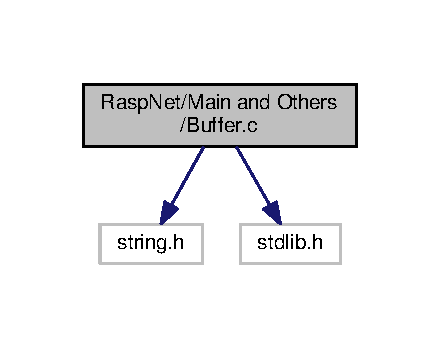
\includegraphics[width=211pt]{Buffer_8c__incl}
\end{center}
\end{figure}
This graph shows which files directly or indirectly include this file\+:
\nopagebreak
\begin{figure}[H]
\begin{center}
\leavevmode
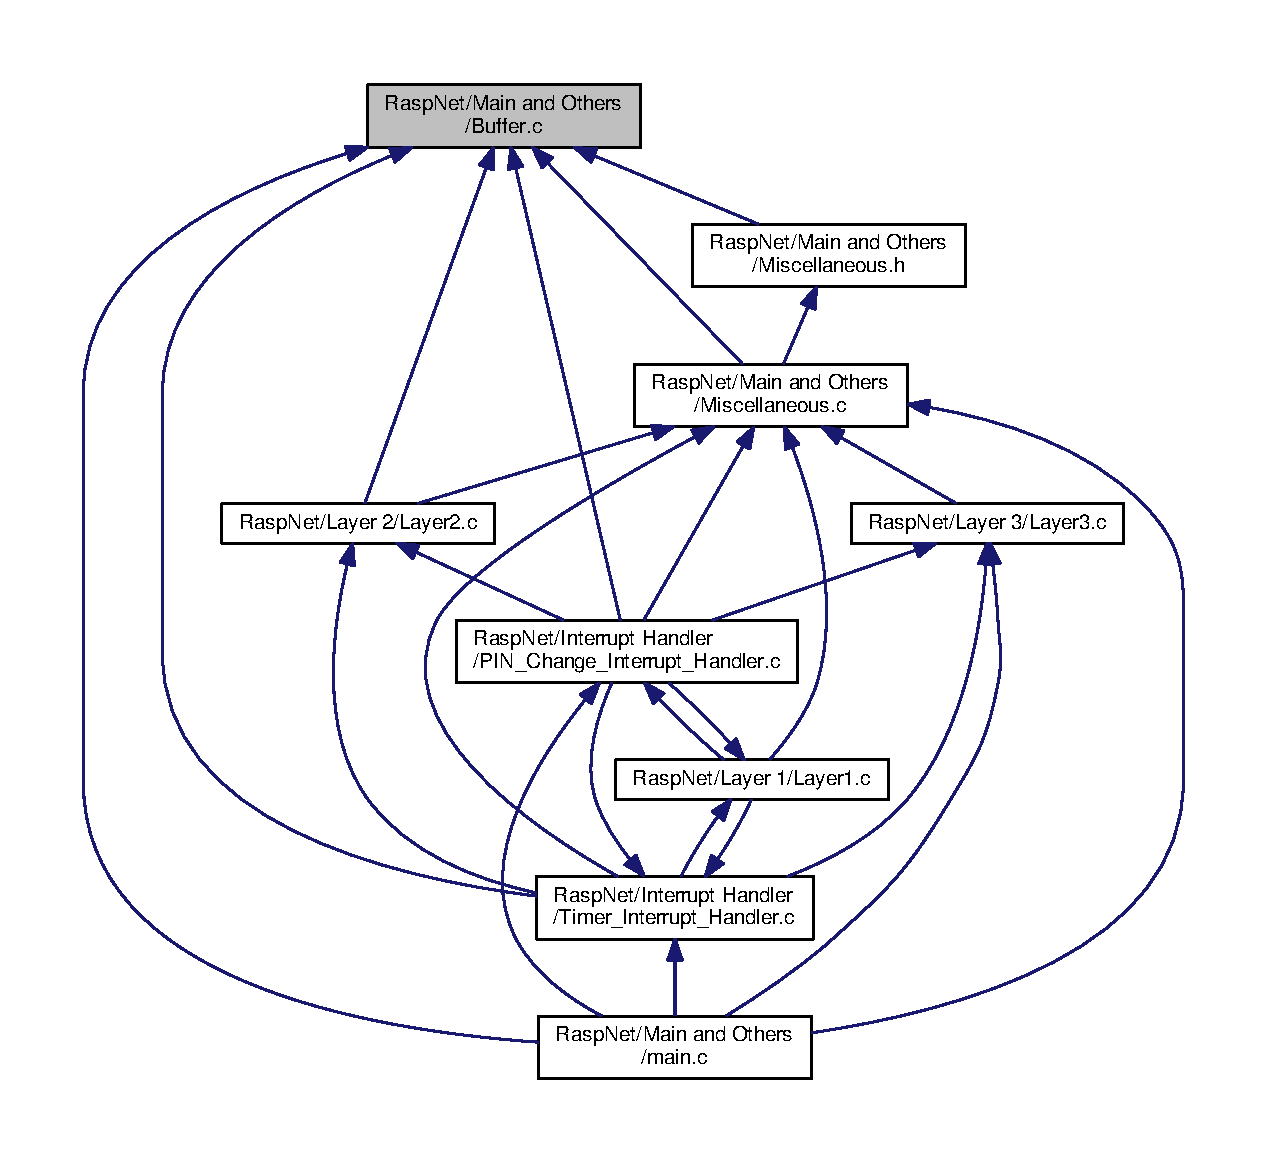
\includegraphics[width=350pt]{Buffer_8c__dep__incl}
\end{center}
\end{figure}
\subsection*{Classes}
\begin{DoxyCompactItemize}
\item 
struct \hyperlink{structPacket}{Packet}
\end{DoxyCompactItemize}
\subsection*{Variables}
\begin{DoxyCompactItemize}
\item 
struct \hyperlink{structPacket}{Packet} transmit\+\_\+packet $\ast$ \hyperlink{Buffer_8c_ac229f7d7f062771563514df9f3927eb6}{transmit\+\_\+packet\+\_\+pointer}
\item 
struct \hyperlink{structPacket}{Packet} receive\+\_\+packet $\ast$ \hyperlink{Buffer_8c_a60b199d535890694c3b1f82494e64e6d}{receive\+\_\+packet\+\_\+pointer}
\item 
struct \hyperlink{structPacket}{Packet} my\+\_\+own\+\_\+packet $\ast$ \hyperlink{Buffer_8c_ac247c7d61e5a6e7abecd95209dae8bcb}{my\+\_\+own\+\_\+packet\+\_\+pointer}
\item 
uint8\+\_\+t \hyperlink{Buffer_8c_ad32f9b2a3c3f3aba80f847dd8c18f77c}{predefined\+\_\+preamble} =0b01111110
\end{DoxyCompactItemize}


\subsection{Variable Documentation}
\index{Buffer.\+c@{Buffer.\+c}!my\+\_\+own\+\_\+packet\+\_\+pointer@{my\+\_\+own\+\_\+packet\+\_\+pointer}}
\index{my\+\_\+own\+\_\+packet\+\_\+pointer@{my\+\_\+own\+\_\+packet\+\_\+pointer}!Buffer.\+c@{Buffer.\+c}}
\subsubsection[{\texorpdfstring{my\+\_\+own\+\_\+packet\+\_\+pointer}{my_own_packet_pointer}}]{\setlength{\rightskip}{0pt plus 5cm}struct {\bf Packet} my\+\_\+own\+\_\+packet$\ast$ my\+\_\+own\+\_\+packet\+\_\+pointer}\hypertarget{Buffer_8c_ac247c7d61e5a6e7abecd95209dae8bcb}{}\label{Buffer_8c_ac247c7d61e5a6e7abecd95209dae8bcb}
My buffer \index{Buffer.\+c@{Buffer.\+c}!predefined\+\_\+preamble@{predefined\+\_\+preamble}}
\index{predefined\+\_\+preamble@{predefined\+\_\+preamble}!Buffer.\+c@{Buffer.\+c}}
\subsubsection[{\texorpdfstring{predefined\+\_\+preamble}{predefined_preamble}}]{\setlength{\rightskip}{0pt plus 5cm}uint8\+\_\+t predefined\+\_\+preamble =0b01111110}\hypertarget{Buffer_8c_ad32f9b2a3c3f3aba80f847dd8c18f77c}{}\label{Buffer_8c_ad32f9b2a3c3f3aba80f847dd8c18f77c}
\index{Buffer.\+c@{Buffer.\+c}!receive\+\_\+packet\+\_\+pointer@{receive\+\_\+packet\+\_\+pointer}}
\index{receive\+\_\+packet\+\_\+pointer@{receive\+\_\+packet\+\_\+pointer}!Buffer.\+c@{Buffer.\+c}}
\subsubsection[{\texorpdfstring{receive\+\_\+packet\+\_\+pointer}{receive_packet_pointer}}]{\setlength{\rightskip}{0pt plus 5cm}struct {\bf Packet} receive\+\_\+packet$\ast$ receive\+\_\+packet\+\_\+pointer}\hypertarget{Buffer_8c_a60b199d535890694c3b1f82494e64e6d}{}\label{Buffer_8c_a60b199d535890694c3b1f82494e64e6d}
Receive buffer \index{Buffer.\+c@{Buffer.\+c}!transmit\+\_\+packet\+\_\+pointer@{transmit\+\_\+packet\+\_\+pointer}}
\index{transmit\+\_\+packet\+\_\+pointer@{transmit\+\_\+packet\+\_\+pointer}!Buffer.\+c@{Buffer.\+c}}
\subsubsection[{\texorpdfstring{transmit\+\_\+packet\+\_\+pointer}{transmit_packet_pointer}}]{\setlength{\rightskip}{0pt plus 5cm}struct {\bf Packet} transmit\+\_\+packet$\ast$ transmit\+\_\+packet\+\_\+pointer}\hypertarget{Buffer_8c_ac229f7d7f062771563514df9f3927eb6}{}\label{Buffer_8c_ac229f7d7f062771563514df9f3927eb6}
Transmit buffer 
\hypertarget{initialization_8c}{}\section{Rasp\+Net/\+Main and Others/initialization.c File Reference}
\label{initialization_8c}\index{Rasp\+Net/\+Main and Others/initialization.\+c@{Rasp\+Net/\+Main and Others/initialization.\+c}}
{\ttfamily \#include $<$avr/io.\+h$>$}\\*
{\ttfamily \#include \char`\"{}initialization.\+h\char`\"{}}\\*
{\ttfamily \#include \char`\"{}U\+A\+R\+T\+\_\+\+Handler.\+h\char`\"{}}\\*
{\ttfamily \#include $<$avr/interrupt.\+h$>$}\\*
Include dependency graph for initialization.\+c\+:
\nopagebreak
\begin{figure}[H]
\begin{center}
\leavevmode
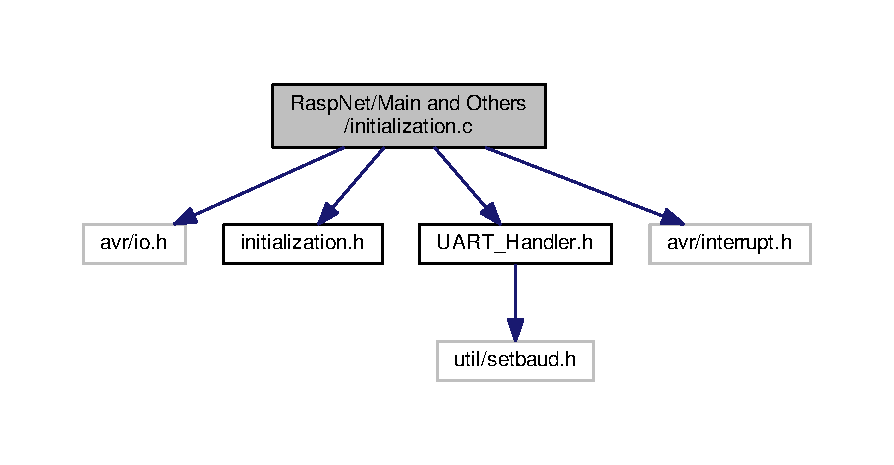
\includegraphics[width=350pt]{initialization_8c__incl}
\end{center}
\end{figure}
This graph shows which files directly or indirectly include this file\+:
\nopagebreak
\begin{figure}[H]
\begin{center}
\leavevmode
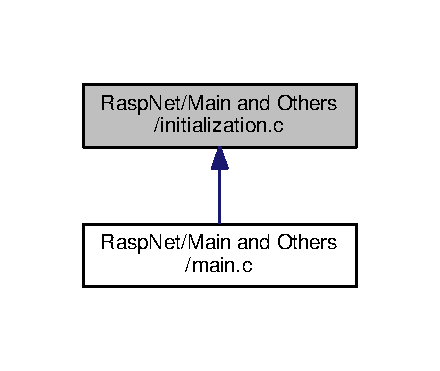
\includegraphics[width=211pt]{initialization_8c__dep__incl}
\end{center}
\end{figure}
\subsection*{Functions}
\begin{DoxyCompactItemize}
\item 
void \hyperlink{initialization_8c_a96e7bed13a0aabf62cd82cb63d0ecdcd}{port\+\_\+initialization} ()
\begin{DoxyCompactList}\small\item\em A\+VR port and pin initialization for input and output purpose. \end{DoxyCompactList}\item 
void \hyperlink{initialization_8c_aa76e84afd914db298418b16267fff5a1}{uart\+\_\+initialization} ()
\begin{DoxyCompactList}\small\item\em U\+A\+RT initialization for serial communication. \end{DoxyCompactList}\item 
void \hyperlink{initialization_8c_af18d14573a8ed7aa3bacc5d77011e423}{timer\+\_\+initialization} ()
\item 
void \hyperlink{initialization_8c_acdf613f8022f5390f71cfeb1e84885c7}{pin\+\_\+change\+\_\+interrupt\+\_\+initialization} ()
\begin{DoxyCompactList}\small\item\em P\+IN change interrupt initialization. \end{DoxyCompactList}\end{DoxyCompactItemize}


\subsection{Function Documentation}
\index{initialization.\+c@{initialization.\+c}!pin\+\_\+change\+\_\+interrupt\+\_\+initialization@{pin\+\_\+change\+\_\+interrupt\+\_\+initialization}}
\index{pin\+\_\+change\+\_\+interrupt\+\_\+initialization@{pin\+\_\+change\+\_\+interrupt\+\_\+initialization}!initialization.\+c@{initialization.\+c}}
\subsubsection[{\texorpdfstring{pin\+\_\+change\+\_\+interrupt\+\_\+initialization()}{pin_change_interrupt_initialization()}}]{\setlength{\rightskip}{0pt plus 5cm}void pin\+\_\+change\+\_\+interrupt\+\_\+initialization (
\begin{DoxyParamCaption}
{}
\end{DoxyParamCaption}
)}\hypertarget{initialization_8c_acdf613f8022f5390f71cfeb1e84885c7}{}\label{initialization_8c_acdf613f8022f5390f71cfeb1e84885c7}


P\+IN change interrupt initialization. 

P\+IN Change interrupt is used for receiving data $<$ enabled P\+C\+I\+NT\mbox{[}23\+:16\mbox{]} pin will cause an interrupt

$<$ pin change interrupt for P\+D4 or clock receive signal 
\begin{DoxyCode}
50                                           \{
51   PCICR|= (1<<PCIE2); 
52   PCMSK2|=(1<<PCINT20);
53 \}
\end{DoxyCode}
\index{initialization.\+c@{initialization.\+c}!port\+\_\+initialization@{port\+\_\+initialization}}
\index{port\+\_\+initialization@{port\+\_\+initialization}!initialization.\+c@{initialization.\+c}}
\subsubsection[{\texorpdfstring{port\+\_\+initialization()}{port_initialization()}}]{\setlength{\rightskip}{0pt plus 5cm}void port\+\_\+initialization (
\begin{DoxyParamCaption}
{}
\end{DoxyParamCaption}
)}\hypertarget{initialization_8c_a96e7bed13a0aabf62cd82cb63d0ecdcd}{}\label{initialization_8c_a96e7bed13a0aabf62cd82cb63d0ecdcd}


A\+VR port and pin initialization for input and output purpose. 

\begin{DoxyReturn}{Returns}
void nothing has to return from this function 
\end{DoxyReturn}
$<$ Receive P\+IN Configuration

$<$ Clock Receive

$<$ Data Receive

$<$ Send P\+IN configuration

$<$ Clock Send

$<$ Data Send

$<$ L\+ED output

$<$ to indicate clock signal receive

$<$ to indicate data signal receive 
\begin{DoxyCode}
7                           \{
9     DDRD&=~(1<<PD4);
10     DDRD&=~(1<<PD5);
13     DDRB|=(1<<PB4);
14     DDRB|=(1<<PB5);
17     DDRB|=(1<<PB3);
18     DDRB|=(1<<PB2);
19 \}
\end{DoxyCode}
\index{initialization.\+c@{initialization.\+c}!timer\+\_\+initialization@{timer\+\_\+initialization}}
\index{timer\+\_\+initialization@{timer\+\_\+initialization}!initialization.\+c@{initialization.\+c}}
\subsubsection[{\texorpdfstring{timer\+\_\+initialization()}{timer_initialization()}}]{\setlength{\rightskip}{0pt plus 5cm}void timer\+\_\+initialization (
\begin{DoxyParamCaption}
{}
\end{DoxyParamCaption}
)}\hypertarget{initialization_8c_af18d14573a8ed7aa3bacc5d77011e423}{}\label{initialization_8c_af18d14573a8ed7aa3bacc5d77011e423}
$<$ Compare match A

$<$ C\+TC mode

$<$ Clock/256 = 46875 (prescalar 256) 
\begin{DoxyCode}
42                            \{
43     TIMSK0 |= (1 << OCIE0A); 
44     TCCR0A |= (1 << WGM01);  
45     TCCR0B |= (1 << CS02);   \textcolor{comment}{//}
46     OCR0A = 0x2f;
47     \textcolor{comment}{//OCR0A = 0x600;}
48 \}
\end{DoxyCode}
\index{initialization.\+c@{initialization.\+c}!uart\+\_\+initialization@{uart\+\_\+initialization}}
\index{uart\+\_\+initialization@{uart\+\_\+initialization}!initialization.\+c@{initialization.\+c}}
\subsubsection[{\texorpdfstring{uart\+\_\+initialization()}{uart_initialization()}}]{\setlength{\rightskip}{0pt plus 5cm}void uart\+\_\+initialization (
\begin{DoxyParamCaption}
{}
\end{DoxyParamCaption}
)}\hypertarget{initialization_8c_aa76e84afd914db298418b16267fff5a1}{}\label{initialization_8c_aa76e84afd914db298418b16267fff5a1}


U\+A\+RT initialization for serial communication. 

\begin{DoxyReturn}{Returns}
void nothing has to return from this function 
\end{DoxyReturn}
$<$ Set baud rate U\+B\+RR is a 16 bit register which is used to set the baud rate of U\+A\+RT

$<$ Transmitter and Receiver is Enabled T\+X\+EN bit 1 Enable Transmission 0 Disable Transmission R\+X\+EN bit 1 Enable Reception 0 Disable Reception

$<$ U\+C\+S\+Z0 and U\+C\+S\+Z1 are used to select the number of data bits to be transmitter

$<$ Asynchornous mode 
\begin{DoxyCode}
21                           \{
26     UBRR0H =  (\textcolor{keywordtype}{unsigned} char)\hyperlink{UART__Handler_8h_a734bbab06e1a9fd2e5522db0221ff6e3}{BAUDRATE}>>8;
27     UBRR0L =  (\textcolor{keywordtype}{unsigned} char)\hyperlink{UART__Handler_8h_a734bbab06e1a9fd2e5522db0221ff6e3}{BAUDRATE};
32     UCSR0B|= (1<<TXEN0)|(1<<RXEN0);
36     UCSR0C|= (1<<USBS0)|(3<<UCSZ00); 
39 \}
\end{DoxyCode}

\hypertarget{initialization_8h}{}\section{Rasp\+Net/\+Main and Others/initialization.h File Reference}
\label{initialization_8h}\index{Rasp\+Net/\+Main and Others/initialization.\+h@{Rasp\+Net/\+Main and Others/initialization.\+h}}
This graph shows which files directly or indirectly include this file\+:
\nopagebreak
\begin{figure}[H]
\begin{center}
\leavevmode
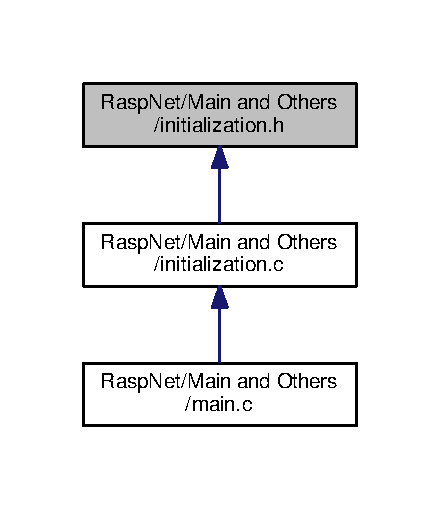
\includegraphics[width=211pt]{initialization_8h__dep__incl}
\end{center}
\end{figure}
\subsection*{Functions}
\begin{DoxyCompactItemize}
\item 
void \hyperlink{initialization_8h_a96e7bed13a0aabf62cd82cb63d0ecdcd}{port\+\_\+initialization} ()
\begin{DoxyCompactList}\small\item\em A\+VR port and pin initialization for input and output purpose. \end{DoxyCompactList}\item 
void \hyperlink{initialization_8h_aa76e84afd914db298418b16267fff5a1}{uart\+\_\+initialization} ()
\begin{DoxyCompactList}\small\item\em U\+A\+RT initialization for serial communication. \end{DoxyCompactList}\item 
void \hyperlink{initialization_8h_a2894de6d2d350b25a70f8cc225768581}{timer\+\_\+interrupt\+\_\+initialization} ()
\begin{DoxyCompactList}\small\item\em Timer register initialization for Timer Interrupt. \end{DoxyCompactList}\item 
void \hyperlink{initialization_8h_acdf613f8022f5390f71cfeb1e84885c7}{pin\+\_\+change\+\_\+interrupt\+\_\+initialization} ()
\begin{DoxyCompactList}\small\item\em P\+IN change interrupt initialization. \end{DoxyCompactList}\end{DoxyCompactItemize}


\subsection{Function Documentation}
\index{initialization.\+h@{initialization.\+h}!pin\+\_\+change\+\_\+interrupt\+\_\+initialization@{pin\+\_\+change\+\_\+interrupt\+\_\+initialization}}
\index{pin\+\_\+change\+\_\+interrupt\+\_\+initialization@{pin\+\_\+change\+\_\+interrupt\+\_\+initialization}!initialization.\+h@{initialization.\+h}}
\subsubsection[{\texorpdfstring{pin\+\_\+change\+\_\+interrupt\+\_\+initialization()}{pin_change_interrupt_initialization()}}]{\setlength{\rightskip}{0pt plus 5cm}void pin\+\_\+change\+\_\+interrupt\+\_\+initialization (
\begin{DoxyParamCaption}
{}
\end{DoxyParamCaption}
)}\hypertarget{initialization_8h_acdf613f8022f5390f71cfeb1e84885c7}{}\label{initialization_8h_acdf613f8022f5390f71cfeb1e84885c7}


P\+IN change interrupt initialization. 

\begin{DoxyReturn}{Returns}
void nothing has to return from this function
\end{DoxyReturn}
P\+IN Change interrupt is used for receiving data $<$ enabled P\+C\+I\+NT\mbox{[}23\+:16\mbox{]} pin will cause an interrupt

$<$ pin change interrupt for P\+D4 or clock receive signal 
\begin{DoxyCode}
50                                           \{
51   PCICR|= (1<<PCIE2); 
52   PCMSK2|=(1<<PCINT20);
53 \}
\end{DoxyCode}
\index{initialization.\+h@{initialization.\+h}!port\+\_\+initialization@{port\+\_\+initialization}}
\index{port\+\_\+initialization@{port\+\_\+initialization}!initialization.\+h@{initialization.\+h}}
\subsubsection[{\texorpdfstring{port\+\_\+initialization()}{port_initialization()}}]{\setlength{\rightskip}{0pt plus 5cm}void port\+\_\+initialization (
\begin{DoxyParamCaption}
{}
\end{DoxyParamCaption}
)}\hypertarget{initialization_8h_a96e7bed13a0aabf62cd82cb63d0ecdcd}{}\label{initialization_8h_a96e7bed13a0aabf62cd82cb63d0ecdcd}


A\+VR port and pin initialization for input and output purpose. 

\begin{DoxyReturn}{Returns}
void nothing has to return from this function 
\end{DoxyReturn}
$<$ Receive P\+IN Configuration

$<$ Clock Receive

$<$ Data Receive

$<$ Send P\+IN configuration

$<$ Clock Send

$<$ Data Send

$<$ L\+ED output

$<$ to indicate clock signal receive

$<$ to indicate data signal receive 
\begin{DoxyCode}
7                           \{
9     DDRD&=~(1<<PD4);
10     DDRD&=~(1<<PD5);
13     DDRB|=(1<<PB4);
14     DDRB|=(1<<PB5);
17     DDRB|=(1<<PB3);
18     DDRB|=(1<<PB2);
19 \}
\end{DoxyCode}
\index{initialization.\+h@{initialization.\+h}!timer\+\_\+interrupt\+\_\+initialization@{timer\+\_\+interrupt\+\_\+initialization}}
\index{timer\+\_\+interrupt\+\_\+initialization@{timer\+\_\+interrupt\+\_\+initialization}!initialization.\+h@{initialization.\+h}}
\subsubsection[{\texorpdfstring{timer\+\_\+interrupt\+\_\+initialization()}{timer_interrupt_initialization()}}]{\setlength{\rightskip}{0pt plus 5cm}void timer\+\_\+interrupt\+\_\+initialization (
\begin{DoxyParamCaption}
{}
\end{DoxyParamCaption}
)}\hypertarget{initialization_8h_a2894de6d2d350b25a70f8cc225768581}{}\label{initialization_8h_a2894de6d2d350b25a70f8cc225768581}


Timer register initialization for Timer Interrupt. 

\begin{DoxyReturn}{Returns}
void nothing has to return from this function 
\end{DoxyReturn}
\index{initialization.\+h@{initialization.\+h}!uart\+\_\+initialization@{uart\+\_\+initialization}}
\index{uart\+\_\+initialization@{uart\+\_\+initialization}!initialization.\+h@{initialization.\+h}}
\subsubsection[{\texorpdfstring{uart\+\_\+initialization()}{uart_initialization()}}]{\setlength{\rightskip}{0pt plus 5cm}void uart\+\_\+initialization (
\begin{DoxyParamCaption}
{}
\end{DoxyParamCaption}
)}\hypertarget{initialization_8h_aa76e84afd914db298418b16267fff5a1}{}\label{initialization_8h_aa76e84afd914db298418b16267fff5a1}


U\+A\+RT initialization for serial communication. 

\begin{DoxyReturn}{Returns}
void nothing has to return from this function 
\end{DoxyReturn}
$<$ Set baud rate U\+B\+RR is a 16 bit register which is used to set the baud rate of U\+A\+RT

$<$ Transmitter and Receiver is Enabled T\+X\+EN bit 1 Enable Transmission 0 Disable Transmission R\+X\+EN bit 1 Enable Reception 0 Disable Reception

$<$ U\+C\+S\+Z0 and U\+C\+S\+Z1 are used to select the number of data bits to be transmitter

$<$ Asynchornous mode 
\begin{DoxyCode}
21                           \{
26     UBRR0H =  (\textcolor{keywordtype}{unsigned} char)\hyperlink{UART__Handler_8h_a734bbab06e1a9fd2e5522db0221ff6e3}{BAUDRATE}>>8;
27     UBRR0L =  (\textcolor{keywordtype}{unsigned} char)\hyperlink{UART__Handler_8h_a734bbab06e1a9fd2e5522db0221ff6e3}{BAUDRATE};
32     UCSR0B|= (1<<TXEN0)|(1<<RXEN0);
36     UCSR0C|= (1<<USBS0)|(3<<UCSZ00); 
39 \}
\end{DoxyCode}

\hypertarget{main_8c}{}\section{Rasp\+Net/\+Main and Others/main.c File Reference}
\label{main_8c}\index{Rasp\+Net/\+Main and Others/main.\+c@{Rasp\+Net/\+Main and Others/main.\+c}}
{\ttfamily \#include $<$avr/io.\+h$>$}\\*
{\ttfamily \#include $<$util/delay.\+h$>$}\\*
{\ttfamily \#include \char`\"{}initialization.\+c\char`\"{}}\\*
{\ttfamily \#include \char`\"{}Timer\+\_\+\+Interrupt\+\_\+\+Handler.\+c\char`\"{}}\\*
{\ttfamily \#include \char`\"{}P\+I\+N\+\_\+\+Change\+\_\+\+Interrupt\+\_\+\+Handler.\+c\char`\"{}}\\*
{\ttfamily \#include \char`\"{}Layer3.\+c\char`\"{}}\\*
{\ttfamily \#include \char`\"{}Buffer.\+c\char`\"{}}\\*
{\ttfamily \#include \char`\"{}Miscellaneous.\+c\char`\"{}}\\*
Include dependency graph for main.\+c\+:
\nopagebreak
\begin{figure}[H]
\begin{center}
\leavevmode
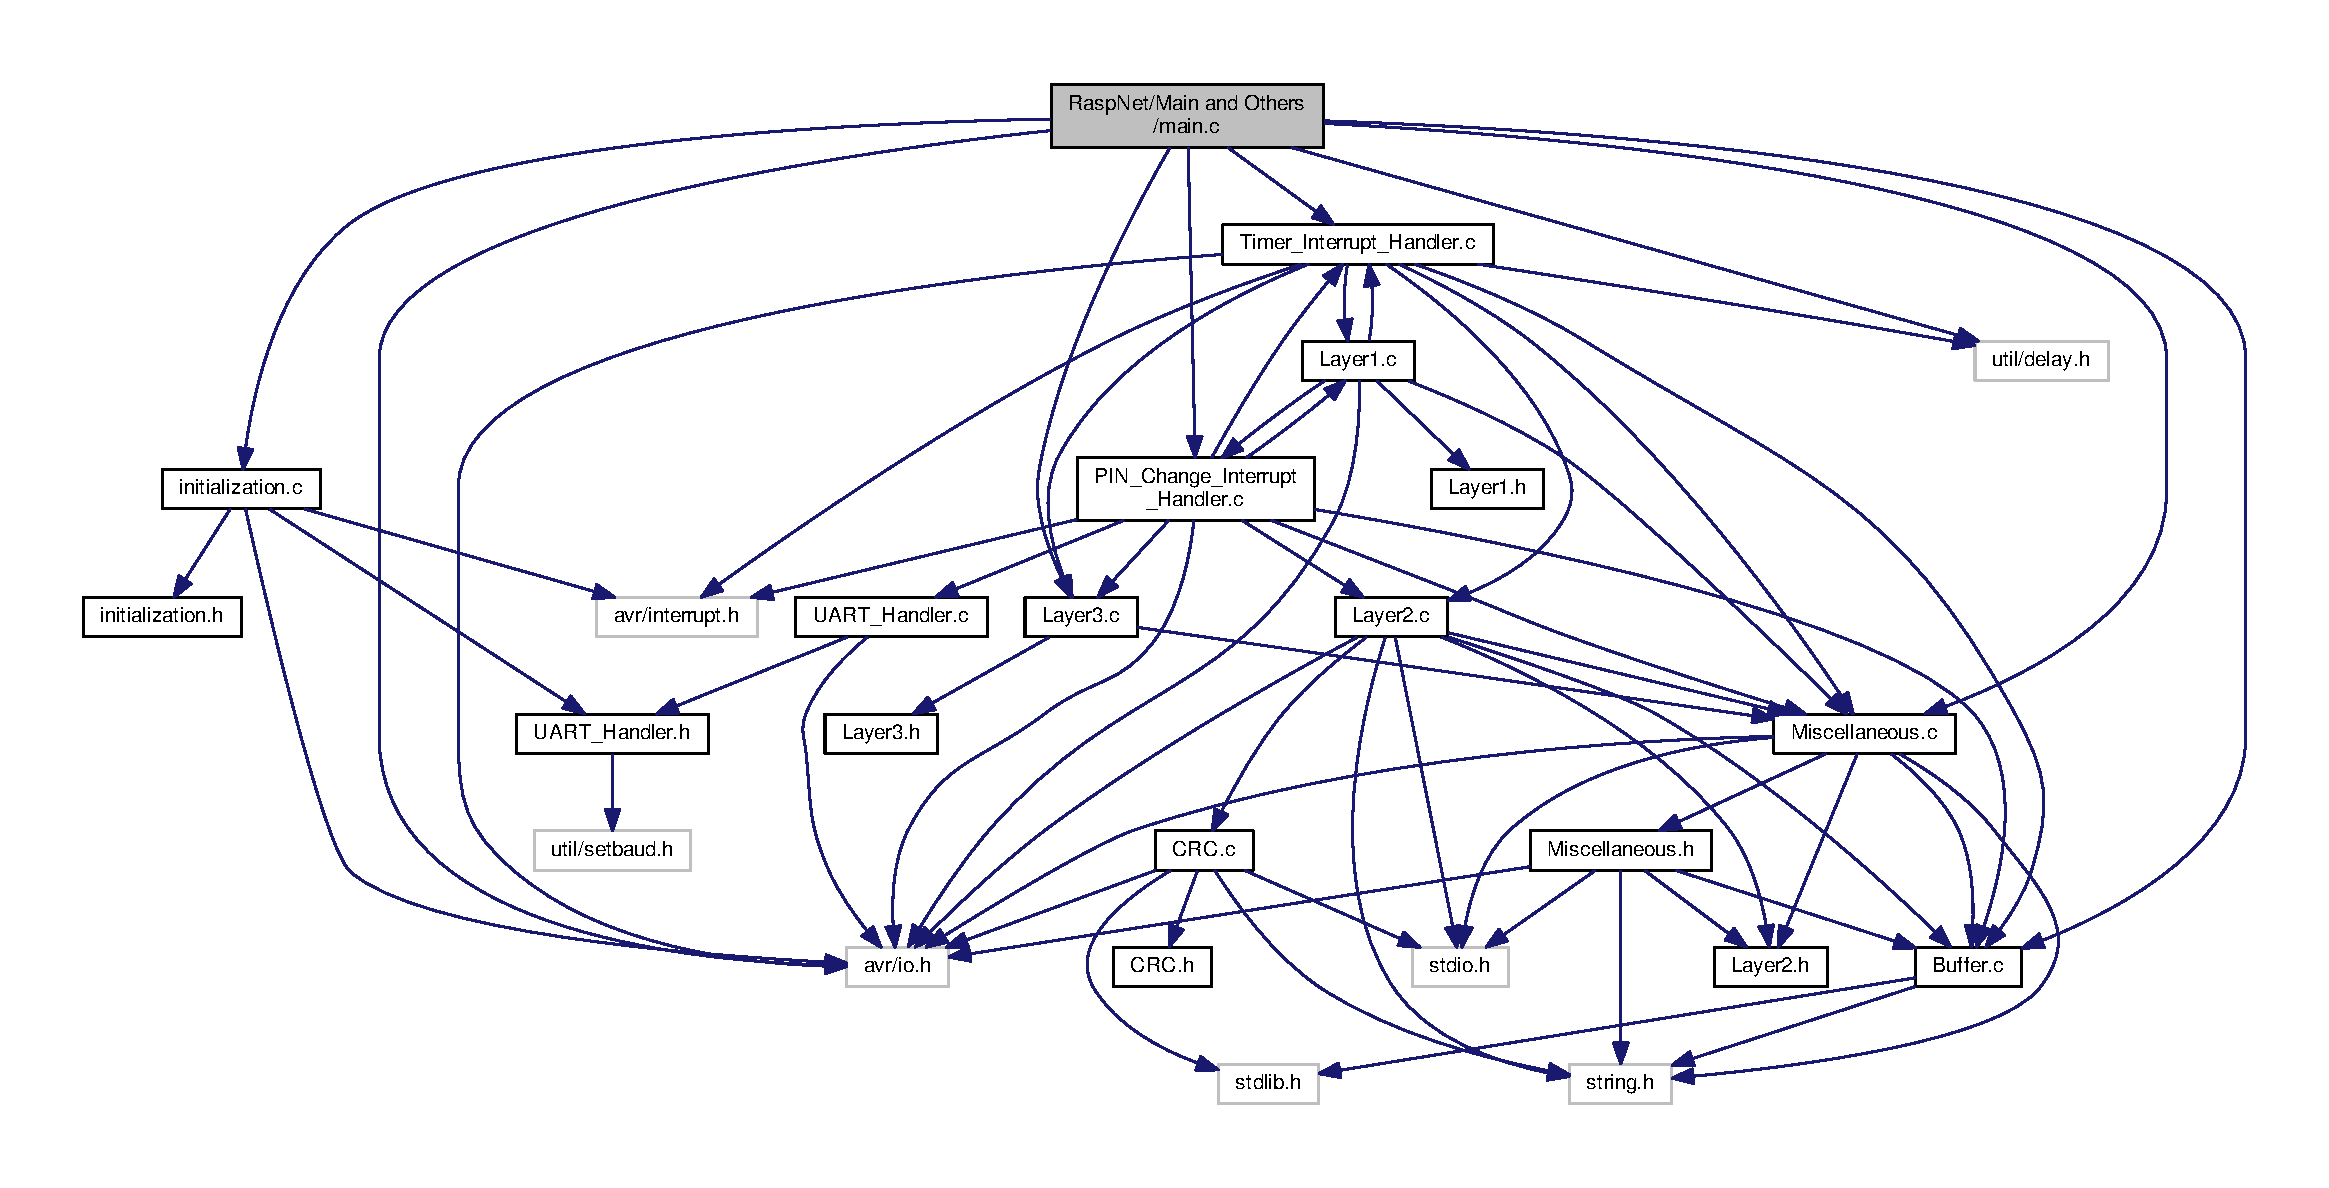
\includegraphics[width=350pt]{main_8c__incl}
\end{center}
\end{figure}
\subsection*{Macros}
\begin{DoxyCompactItemize}
\item 
\#define \hyperlink{main_8c_a43bafb28b29491ec7f871319b5a3b2f8}{F\+\_\+\+C\+PU}~16000000\+UL
\end{DoxyCompactItemize}
\subsection*{Functions}
\begin{DoxyCompactItemize}
\item 
int \hyperlink{main_8c_ae66f6b31b5ad750f1fe042a706a4e3d4}{main} ()
\end{DoxyCompactItemize}


\subsection{Macro Definition Documentation}
\index{main.\+c@{main.\+c}!F\+\_\+\+C\+PU@{F\+\_\+\+C\+PU}}
\index{F\+\_\+\+C\+PU@{F\+\_\+\+C\+PU}!main.\+c@{main.\+c}}
\subsubsection[{\texorpdfstring{F\+\_\+\+C\+PU}{F_CPU}}]{\setlength{\rightskip}{0pt plus 5cm}\#define F\+\_\+\+C\+PU~16000000\+UL}\hypertarget{main_8c_a43bafb28b29491ec7f871319b5a3b2f8}{}\label{main_8c_a43bafb28b29491ec7f871319b5a3b2f8}


\subsection{Function Documentation}
\index{main.\+c@{main.\+c}!main@{main}}
\index{main@{main}!main.\+c@{main.\+c}}
\subsubsection[{\texorpdfstring{main()}{main()}}]{\setlength{\rightskip}{0pt plus 5cm}int main (
\begin{DoxyParamCaption}
{}
\end{DoxyParamCaption}
)}\hypertarget{main_8c_ae66f6b31b5ad750f1fe042a706a4e3d4}{}\label{main_8c_ae66f6b31b5ad750f1fe042a706a4e3d4}
$<$ Initialization

$<$ Global interrupt

$<$ Fill with payload data

$<$ Fill buffer with predefined data 
\begin{DoxyCode}
13           \{
15     \hyperlink{initialization_8c_a96e7bed13a0aabf62cd82cb63d0ecdcd}{port\_initialization}();
16     \hyperlink{initialization_8c_aa76e84afd914db298418b16267fff5a1}{uart\_initialization}();
17     \hyperlink{PIN__Change__Interrupt__Handler_8c_acdf613f8022f5390f71cfeb1e84885c7}{pin\_change\_interrupt\_initialization}();
18     \hyperlink{initialization_8c_af18d14573a8ed7aa3bacc5d77011e423}{timer\_initialization}();
19     sei();
23     \hyperlink{Buffer_8c_ac229f7d7f062771563514df9f3927eb6}{transmit\_packet\_pointer}=&transmit\_packet;
24     \hyperlink{Buffer_8c_a60b199d535890694c3b1f82494e64e6d}{receive\_packet\_pointer}=&receive\_packet;
25     \hyperlink{Buffer_8c_ac247c7d61e5a6e7abecd95209dae8bcb}{my\_own\_packet\_pointer}=&my\_own\_packet;
26     \hyperlink{Buffer_8c_ac247c7d61e5a6e7abecd95209dae8bcb}{my\_own\_packet\_pointer}->\hyperlink{structPacket_a01308f5b690e5060fea6037e765058b9}{source}=0x3;
27     \hyperlink{Buffer_8c_ac247c7d61e5a6e7abecd95209dae8bcb}{my\_own\_packet\_pointer}->\hyperlink{structPacket_af626fe07d93fe4116d613304792df080}{destination}=0x4;
28     uint8\_t payload\_data[6]=\{\hyperlink{Buffer_8c_ac247c7d61e5a6e7abecd95209dae8bcb}{my\_own\_packet\_pointer}->
      \hyperlink{structPacket_af626fe07d93fe4116d613304792df080}{destination},\hyperlink{Buffer_8c_ac247c7d61e5a6e7abecd95209dae8bcb}{my\_own\_packet\_pointer}->\hyperlink{structPacket_a01308f5b690e5060fea6037e765058b9}{source},0x74,0x65,0x73,0x74\}; 
31     \hyperlink{Buffer_8c_ac247c7d61e5a6e7abecd95209dae8bcb}{my\_own\_packet\_pointer}->\hyperlink{structPacket_aa305c88136c91911a5159610863cb41d}{preamble}=
      \hyperlink{Buffer_8c_ad32f9b2a3c3f3aba80f847dd8c18f77c}{predefined\_preamble};
32     \hyperlink{Buffer_8c_ac247c7d61e5a6e7abecd95209dae8bcb}{my\_own\_packet\_pointer}->\hyperlink{structPacket_a58a48ac639979f488f254bbcb98e72b8}{payload}[0]=payload\_data[0];
33     \hyperlink{Buffer_8c_ac247c7d61e5a6e7abecd95209dae8bcb}{my\_own\_packet\_pointer}->\hyperlink{structPacket_a58a48ac639979f488f254bbcb98e72b8}{payload}[1]=payload\_data[1];
34     \hyperlink{Buffer_8c_ac247c7d61e5a6e7abecd95209dae8bcb}{my\_own\_packet\_pointer}->\hyperlink{structPacket_a58a48ac639979f488f254bbcb98e72b8}{payload}[2]=payload\_data[2];
35     \hyperlink{Buffer_8c_ac247c7d61e5a6e7abecd95209dae8bcb}{my\_own\_packet\_pointer}->\hyperlink{structPacket_a58a48ac639979f488f254bbcb98e72b8}{payload}[3]=payload\_data[3];
36     \hyperlink{Buffer_8c_ac247c7d61e5a6e7abecd95209dae8bcb}{my\_own\_packet\_pointer}->\hyperlink{structPacket_a58a48ac639979f488f254bbcb98e72b8}{payload}[4]=payload\_data[4];
37     \hyperlink{Buffer_8c_ac247c7d61e5a6e7abecd95209dae8bcb}{my\_own\_packet\_pointer}->\hyperlink{structPacket_a58a48ac639979f488f254bbcb98e72b8}{payload}[5]=payload\_data[5];
38     \hyperlink{Buffer_8c_ac247c7d61e5a6e7abecd95209dae8bcb}{my\_own\_packet\_pointer}->\hyperlink{structPacket_ab13014675ea9eda122b1c50842a567fc}{payload\_siz}= 0x6;
39     \hyperlink{Buffer_8c_ac247c7d61e5a6e7abecd95209dae8bcb}{my\_own\_packet\_pointer}->\hyperlink{structPacket_abad95795e9615463d9d69d298a86b0b8}{crc}=\hyperlink{CRC_8c_a80a6d5b0482ae9760e75c021a70a4ce1}{CRC\_Computation}(
      \hyperlink{Buffer_8c_ac247c7d61e5a6e7abecd95209dae8bcb}{my\_own\_packet\_pointer}->\hyperlink{structPacket_a58a48ac639979f488f254bbcb98e72b8}{payload},\hyperlink{Buffer_8c_ac247c7d61e5a6e7abecd95209dae8bcb}{my\_own\_packet\_pointer}->
      \hyperlink{structPacket_ab13014675ea9eda122b1c50842a567fc}{payload\_siz});
40     \hyperlink{PIN__Change__Interrupt__Handler_8c_a7931d58a3bd94b4566da60f28597d922}{receiver\_flag}=\hyperlink{Layer3_8h_aa8ef63ae0468c77b8312b92d7154609d}{receive\_preamble};
41 
42     \textcolor{keywordflow}{while}(1)\{
43 
44 
45         \textcolor{keywordflow}{while}((\hyperlink{Layer3_8h_a2a0eb18d69ebbaf44dd4e863fa4f6a59}{priority\_type}==\hyperlink{Layer3_8h_aaccf0a951ca84ac3578fa3bcfbac5522}{priority\_for\_relay})||(
      \hyperlink{Layer3_8h_a2a0eb18d69ebbaf44dd4e863fa4f6a59}{priority\_type}==\hyperlink{Layer3_8h_a3b7ed14628679beda488dc3269b7b6a0}{priority\_for\_sending\_order})||(
      \hyperlink{Layer3_8h_a2a0eb18d69ebbaf44dd4e863fa4f6a59}{priority\_type}==\hyperlink{Layer3_8h_a4a793a607f3e830119fe598d76630898}{priority\_high}));
46         \hyperlink{Miscellaneous_8c_afac087d6e168f5fc2cd8994eb07eadb2}{showLog}(\textcolor{stringliteral}{"------------------------------Rafiqul Islam-----------------------"});
47         \hyperlink{Layer3_8h_a2a0eb18d69ebbaf44dd4e863fa4f6a59}{priority\_type}=\hyperlink{Layer3_8h_a3b7ed14628679beda488dc3269b7b6a0}{priority\_for\_sending\_order};
48         *\hyperlink{Buffer_8c_ac229f7d7f062771563514df9f3927eb6}{transmit\_packet\_pointer}= *\hyperlink{Buffer_8c_ac247c7d61e5a6e7abecd95209dae8bcb}{my\_own\_packet\_pointer};
49         \hyperlink{PIN__Change__Interrupt__Handler_8c_a84100ed1f53f510ef91a3d88f24b4b53}{sender\_flag}=\hyperlink{Layer3_8h_a5b4f913d88d52723f970056a0ea4dd09}{transmit\_preamble};
50         \textcolor{comment}{//\_delay\_ms(100);}
51 
52 
53 
54     \}
55 
56     \textcolor{keywordflow}{return} 0;
57 \}
\end{DoxyCode}

\hypertarget{Miscellaneous_8c}{}\section{Rasp\+Net/\+Main and Others/\+Miscellaneous.c File Reference}
\label{Miscellaneous_8c}\index{Rasp\+Net/\+Main and Others/\+Miscellaneous.\+c@{Rasp\+Net/\+Main and Others/\+Miscellaneous.\+c}}
{\ttfamily \#include $<$avr/io.\+h$>$}\\*
{\ttfamily \#include $<$stdio.\+h$>$}\\*
{\ttfamily \#include $<$string.\+h$>$}\\*
{\ttfamily \#include \char`\"{}Buffer.\+c\char`\"{}}\\*
{\ttfamily \#include \char`\"{}Layer2.\+h\char`\"{}}\\*
{\ttfamily \#include \char`\"{}Miscellaneous.\+h\char`\"{}}\\*
Include dependency graph for Miscellaneous.\+c\+:
\nopagebreak
\begin{figure}[H]
\begin{center}
\leavevmode
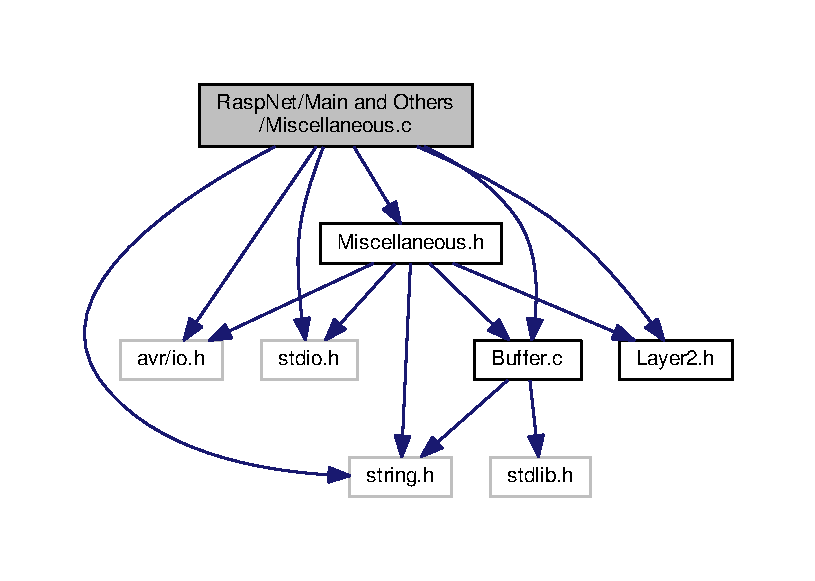
\includegraphics[width=350pt]{Miscellaneous_8c__incl}
\end{center}
\end{figure}
This graph shows which files directly or indirectly include this file\+:
\nopagebreak
\begin{figure}[H]
\begin{center}
\leavevmode
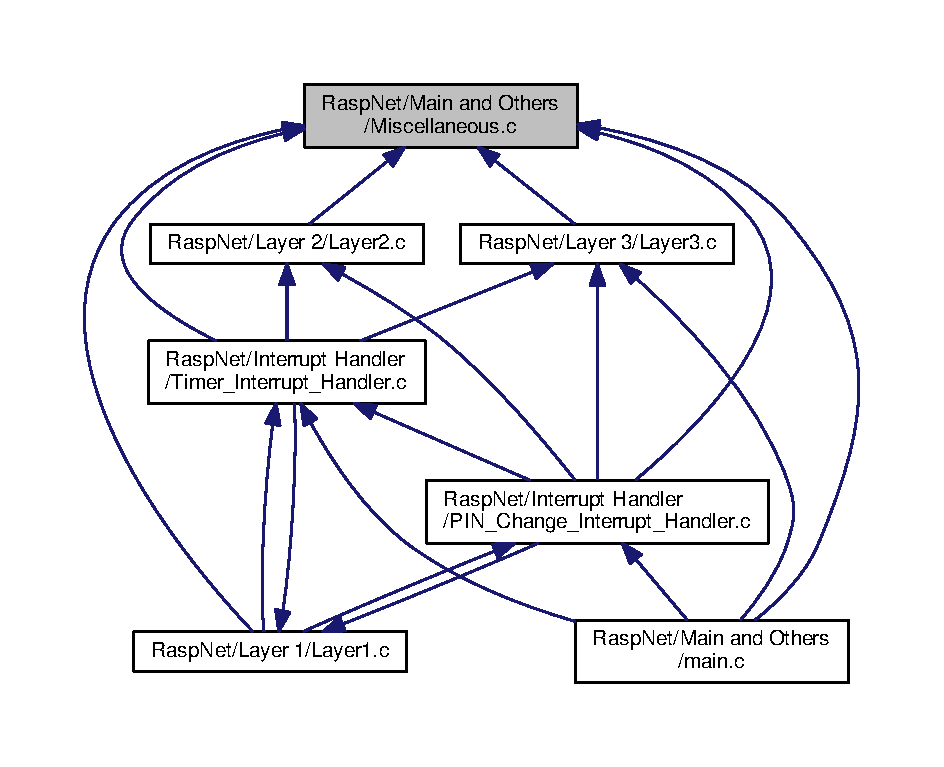
\includegraphics[width=350pt]{Miscellaneous_8c__dep__incl}
\end{center}
\end{figure}
\subsection*{Functions}
\begin{DoxyCompactItemize}
\item 
int \hyperlink{Miscellaneous_8c_a3c3d2514913829c2be8324680f0987b9}{read\+\_\+8\+\_\+bit} (uint8\+\_\+t bits, int pos)
\begin{DoxyCompactList}\small\item\em Read from 8 bit unsigned integer. \end{DoxyCompactList}\item 
int \hyperlink{Miscellaneous_8c_a027b54125044a7b75a94ebdfef27ab46}{read\+\_\+32\+\_\+bit} (uint32\+\_\+t bits, int pos)
\begin{DoxyCompactList}\small\item\em Read from 32 bit unsigned integer. \end{DoxyCompactList}\item 
uint8\+\_\+t \hyperlink{Miscellaneous_8c_af81f6965e50b219ff38ea272019bac1f}{write\+\_\+8\+\_\+bit} (uint8\+\_\+t value, int pos, int value\+\_\+to\+\_\+write)
\begin{DoxyCompactList}\small\item\em Write in 8 bit unsigned integer. \end{DoxyCompactList}\item 
uint32\+\_\+t \hyperlink{Miscellaneous_8c_a864fd2a5d36c61fdc91090a497784b55}{write\+\_\+32\+\_\+bit} (uint32\+\_\+t value, int pos, int value\+\_\+to\+\_\+write)
\begin{DoxyCompactList}\small\item\em Write in 32 bit unsigned integer. \end{DoxyCompactList}\item 
void \hyperlink{Miscellaneous_8c_afac087d6e168f5fc2cd8994eb07eadb2}{show\+Log} (char msg\mbox{[}$\,$\mbox{]})
\begin{DoxyCompactList}\small\item\em Display message consists of string. \end{DoxyCompactList}\item 
int \hyperlink{Miscellaneous_8c_ad063f3ce115eb187d5cbb6fd2b00c0e6}{compare\+\_\+preamble} (uint8\+\_\+t a, uint8\+\_\+t b)
\begin{DoxyCompactList}\small\item\em Compare between received preamble and predefined preamble. \end{DoxyCompactList}\item 
void \hyperlink{Miscellaneous_8c_ae61d07597b559d7305b272b31507f138}{show\+\_\+8\+\_\+bit\+\_\+data} (uint8\+\_\+t data)
\item 
void \hyperlink{Miscellaneous_8c_a4da719f1865290663e587ffb1b00744d}{show\+\_\+32\+\_\+bit\+\_\+data} (uint32\+\_\+t data)
\item 
void \hyperlink{Miscellaneous_8c_a9ea1d4b6a27b5caa55c150b2ba17983a}{show\+\_\+payload} (uint8\+\_\+t $\ast$data, uint8\+\_\+t length)
\begin{DoxyCompactList}\small\item\em Display payload message. \end{DoxyCompactList}\item 
int \hyperlink{Miscellaneous_8c_a7ea454e652a249ba5f17f6233e65887a}{compare\+\_\+crc} (uint32\+\_\+t a, uint32\+\_\+t b)
\begin{DoxyCompactList}\small\item\em Compare between received C\+RC and generated C\+RC from payload. \end{DoxyCompactList}\end{DoxyCompactItemize}


\subsection{Function Documentation}
\index{Miscellaneous.\+c@{Miscellaneous.\+c}!compare\+\_\+crc@{compare\+\_\+crc}}
\index{compare\+\_\+crc@{compare\+\_\+crc}!Miscellaneous.\+c@{Miscellaneous.\+c}}
\subsubsection[{\texorpdfstring{compare\+\_\+crc(uint32\+\_\+t a, uint32\+\_\+t b)}{compare_crc(uint32_t a, uint32_t b)}}]{\setlength{\rightskip}{0pt plus 5cm}int compare\+\_\+crc (
\begin{DoxyParamCaption}
\item[{uint32\+\_\+t}]{a, }
\item[{uint32\+\_\+t}]{b}
\end{DoxyParamCaption}
)}\hypertarget{Miscellaneous_8c_a7ea454e652a249ba5f17f6233e65887a}{}\label{Miscellaneous_8c_a7ea454e652a249ba5f17f6233e65887a}


Compare between received C\+RC and generated C\+RC from payload. 


\begin{DoxyParams}{Parameters}
{\em a} & 32 bit unsigned integer, which is generated from the payload \\
\hline
{\em b} & 32 bit unsigned integer, which is received \\
\hline
\end{DoxyParams}
\begin{DoxyReturn}{Returns}
int data, which is 1 if match otherwise, 0 if does not match 
\end{DoxyReturn}
$<$ Bit compare using X\+OR

$<$ O X\+OR 1 = 1

$<$ O X\+OR 0 = 0, 1 X\+OR 1 = 0 
\begin{DoxyCode}
132                                         \{
133     \textcolor{keywordflow}{if}(!(a^b)) \{    
134         \textcolor{keywordflow}{return} 1;   
135     \}
136     \textcolor{keywordflow}{else} \{
137         \textcolor{keywordflow}{return} 0;   
138     \}
139 \}
\end{DoxyCode}
\index{Miscellaneous.\+c@{Miscellaneous.\+c}!compare\+\_\+preamble@{compare\+\_\+preamble}}
\index{compare\+\_\+preamble@{compare\+\_\+preamble}!Miscellaneous.\+c@{Miscellaneous.\+c}}
\subsubsection[{\texorpdfstring{compare\+\_\+preamble(uint8\+\_\+t a, uint8\+\_\+t b)}{compare_preamble(uint8_t a, uint8_t b)}}]{\setlength{\rightskip}{0pt plus 5cm}int compare\+\_\+preamble (
\begin{DoxyParamCaption}
\item[{uint8\+\_\+t}]{a, }
\item[{uint8\+\_\+t}]{b}
\end{DoxyParamCaption}
)}\hypertarget{Miscellaneous_8c_ad063f3ce115eb187d5cbb6fd2b00c0e6}{}\label{Miscellaneous_8c_ad063f3ce115eb187d5cbb6fd2b00c0e6}


Compare between received preamble and predefined preamble. 


\begin{DoxyParams}{Parameters}
{\em a} & 8 bit unsigned integer, which is predefined \\
\hline
{\em b} & 8 bit unsigned integer, which is received \\
\hline
\end{DoxyParams}
\begin{DoxyReturn}{Returns}
int data, which is 1 if match otherwise, 0 if does not match 
\end{DoxyReturn}
$<$ Bit compare using X\+OR

$<$ O X\+OR 1 = 1

$<$ O X\+OR 0 = 0, 1 X\+OR 1 = 0 
\begin{DoxyCode}
71                                            \{
72     \textcolor{keywordflow}{if}(!(a^b)) \{                 
73         \textcolor{keywordflow}{return} 1;                
74     \}
75     \textcolor{keywordflow}{else} \{
76         \textcolor{keywordflow}{return} 0;                
77     \}
78 \}
\end{DoxyCode}
\index{Miscellaneous.\+c@{Miscellaneous.\+c}!read\+\_\+32\+\_\+bit@{read\+\_\+32\+\_\+bit}}
\index{read\+\_\+32\+\_\+bit@{read\+\_\+32\+\_\+bit}!Miscellaneous.\+c@{Miscellaneous.\+c}}
\subsubsection[{\texorpdfstring{read\+\_\+32\+\_\+bit(uint32\+\_\+t bits, int pos)}{read_32_bit(uint32_t bits, int pos)}}]{\setlength{\rightskip}{0pt plus 5cm}int read\+\_\+32\+\_\+bit (
\begin{DoxyParamCaption}
\item[{uint32\+\_\+t}]{bits, }
\item[{int}]{pos}
\end{DoxyParamCaption}
)}\hypertarget{Miscellaneous_8c_a027b54125044a7b75a94ebdfef27ab46}{}\label{Miscellaneous_8c_a027b54125044a7b75a94ebdfef27ab46}


Read from 32 bit unsigned integer. 


\begin{DoxyParams}{Parameters}
{\em bits} & The 32 bit integer to read to \\
\hline
{\em pos} & Read bit at particular position \\
\hline
\end{DoxyParams}
\begin{DoxyReturn}{Returns}
int data which are 1 or 0 
\end{DoxyReturn}
$<$ Casting and left shift 
\begin{DoxyCode}
21                                         \{
22     uint32\_t mask;
23     mask=((uint32\_t)0x00000001) << pos; 
24     \textcolor{keywordflow}{if}(bits&mask) \{
25         \textcolor{keywordflow}{return} 1;
26     \}
27     \textcolor{keywordflow}{else} \{
28         \textcolor{keywordflow}{return} 0;
29     \}
30 \}
\end{DoxyCode}
\index{Miscellaneous.\+c@{Miscellaneous.\+c}!read\+\_\+8\+\_\+bit@{read\+\_\+8\+\_\+bit}}
\index{read\+\_\+8\+\_\+bit@{read\+\_\+8\+\_\+bit}!Miscellaneous.\+c@{Miscellaneous.\+c}}
\subsubsection[{\texorpdfstring{read\+\_\+8\+\_\+bit(uint8\+\_\+t bits, int pos)}{read_8_bit(uint8_t bits, int pos)}}]{\setlength{\rightskip}{0pt plus 5cm}int read\+\_\+8\+\_\+bit (
\begin{DoxyParamCaption}
\item[{uint8\+\_\+t}]{bits, }
\item[{int}]{pos}
\end{DoxyParamCaption}
)}\hypertarget{Miscellaneous_8c_a3c3d2514913829c2be8324680f0987b9}{}\label{Miscellaneous_8c_a3c3d2514913829c2be8324680f0987b9}


Read from 8 bit unsigned integer. 

$<$ allows to include header file when needed otherwise ignore $<$ Left shift based on pos value

$<$ Logical \& to check bit at particular position 
\begin{DoxyCode}
11                                       \{
12     pos=(1<<pos); 
13     \textcolor{keywordflow}{if}(bits&pos) \{ 
14         \textcolor{keywordflow}{return} 1;
15     \}
16     \textcolor{keywordflow}{else} \{
17         \textcolor{keywordflow}{return} 0;
18     \}
19 \}
\end{DoxyCode}
\index{Miscellaneous.\+c@{Miscellaneous.\+c}!show\+\_\+32\+\_\+bit\+\_\+data@{show\+\_\+32\+\_\+bit\+\_\+data}}
\index{show\+\_\+32\+\_\+bit\+\_\+data@{show\+\_\+32\+\_\+bit\+\_\+data}!Miscellaneous.\+c@{Miscellaneous.\+c}}
\subsubsection[{\texorpdfstring{show\+\_\+32\+\_\+bit\+\_\+data(uint32\+\_\+t data)}{show_32_bit_data(uint32_t data)}}]{\setlength{\rightskip}{0pt plus 5cm}void show\+\_\+32\+\_\+bit\+\_\+data (
\begin{DoxyParamCaption}
\item[{uint32\+\_\+t}]{data}
\end{DoxyParamCaption}
)}\hypertarget{Miscellaneous_8c_a4da719f1865290663e587ffb1b00744d}{}\label{Miscellaneous_8c_a4da719f1865290663e587ffb1b00744d}
$<$ Read from M\+SB

$<$ Read data at particular position

$<$ Display 1

$<$ Display 0 
\begin{DoxyCode}
96                                      \{
97     \textcolor{keywordtype}{int} i;
98     \hyperlink{Miscellaneous_8h_ade3319d0c8a73744f47a483a8816cabe}{uart\_transmission}(\textcolor{charliteral}{'\(\backslash\)n'});
99     \hyperlink{Miscellaneous_8h_ade3319d0c8a73744f47a483a8816cabe}{uart\_transmission}(\textcolor{charliteral}{'\(\backslash\)r'});
100     \textcolor{keywordflow}{for}(i=31; i>=0; i--) \{       
101         \textcolor{keywordflow}{if}(\hyperlink{Miscellaneous_8c_a027b54125044a7b75a94ebdfef27ab46}{read\_32\_bit}(data,i)) \{ 
102             \hyperlink{Miscellaneous_8h_ade3319d0c8a73744f47a483a8816cabe}{uart\_transmission}(\textcolor{charliteral}{'1'}); 
103         \}
104         \textcolor{keywordflow}{else} \{
105             \hyperlink{Miscellaneous_8h_ade3319d0c8a73744f47a483a8816cabe}{uart\_transmission}(\textcolor{charliteral}{'0'}); 
106         \}
107     \}
108     \hyperlink{Miscellaneous_8h_ade3319d0c8a73744f47a483a8816cabe}{uart\_transmission}(\textcolor{charliteral}{'\(\backslash\)n'});
109     \hyperlink{Miscellaneous_8h_ade3319d0c8a73744f47a483a8816cabe}{uart\_transmission}(\textcolor{charliteral}{'\(\backslash\)r'});
110 \}
\end{DoxyCode}
\index{Miscellaneous.\+c@{Miscellaneous.\+c}!show\+\_\+8\+\_\+bit\+\_\+data@{show\+\_\+8\+\_\+bit\+\_\+data}}
\index{show\+\_\+8\+\_\+bit\+\_\+data@{show\+\_\+8\+\_\+bit\+\_\+data}!Miscellaneous.\+c@{Miscellaneous.\+c}}
\subsubsection[{\texorpdfstring{show\+\_\+8\+\_\+bit\+\_\+data(uint8\+\_\+t data)}{show_8_bit_data(uint8_t data)}}]{\setlength{\rightskip}{0pt plus 5cm}void show\+\_\+8\+\_\+bit\+\_\+data (
\begin{DoxyParamCaption}
\item[{uint8\+\_\+t}]{data}
\end{DoxyParamCaption}
)}\hypertarget{Miscellaneous_8c_ae61d07597b559d7305b272b31507f138}{}\label{Miscellaneous_8c_ae61d07597b559d7305b272b31507f138}
$<$ Read from M\+SB

$<$ Read data at particular position

$<$ Display 1

$<$ Display 0 
\begin{DoxyCode}
80                                    \{
81     \textcolor{keywordtype}{int} i;
82     \hyperlink{Miscellaneous_8h_ade3319d0c8a73744f47a483a8816cabe}{uart\_transmission}(\textcolor{charliteral}{'\(\backslash\)n'});
83     \hyperlink{Miscellaneous_8h_ade3319d0c8a73744f47a483a8816cabe}{uart\_transmission}(\textcolor{charliteral}{'\(\backslash\)r'});
84     \textcolor{keywordflow}{for}(i=7; i>=0; i--) \{       
85         \textcolor{keywordflow}{if}(\hyperlink{Miscellaneous_8c_a3c3d2514913829c2be8324680f0987b9}{read\_8\_bit}(data,i)) \{ 
86             \hyperlink{Miscellaneous_8h_ade3319d0c8a73744f47a483a8816cabe}{uart\_transmission}(\textcolor{charliteral}{'1'}); 
87         \}
88         \textcolor{keywordflow}{else} \{
89             \hyperlink{Miscellaneous_8h_ade3319d0c8a73744f47a483a8816cabe}{uart\_transmission}(\textcolor{charliteral}{'0'}); 
90         \}
91     \}
92     \hyperlink{Miscellaneous_8h_ade3319d0c8a73744f47a483a8816cabe}{uart\_transmission}(\textcolor{charliteral}{'\(\backslash\)n'});
93     \hyperlink{Miscellaneous_8h_ade3319d0c8a73744f47a483a8816cabe}{uart\_transmission}(\textcolor{charliteral}{'\(\backslash\)r'});
94 \}
\end{DoxyCode}
\index{Miscellaneous.\+c@{Miscellaneous.\+c}!show\+\_\+payload@{show\+\_\+payload}}
\index{show\+\_\+payload@{show\+\_\+payload}!Miscellaneous.\+c@{Miscellaneous.\+c}}
\subsubsection[{\texorpdfstring{show\+\_\+payload(uint8\+\_\+t $\ast$data, uint8\+\_\+t length)}{show_payload(uint8_t *data, uint8_t length)}}]{\setlength{\rightskip}{0pt plus 5cm}void show\+\_\+payload (
\begin{DoxyParamCaption}
\item[{uint8\+\_\+t $\ast$}]{data, }
\item[{uint8\+\_\+t}]{length}
\end{DoxyParamCaption}
)}\hypertarget{Miscellaneous_8c_a9ea1d4b6a27b5caa55c150b2ba17983a}{}\label{Miscellaneous_8c_a9ea1d4b6a27b5caa55c150b2ba17983a}


Display payload message. 


\begin{DoxyParams}{Parameters}
{\em data} & 8 bit unsigned character array \\
\hline
{\em length} & Length of the payload \\
\hline
\end{DoxyParams}
\begin{DoxyReturn}{Returns}
void nothing has to return 
\end{DoxyReturn}
$<$ Iterate over every element of the array

$<$ Read from the M\+SB

$<$ Display 1

$<$ Display 0 
\begin{DoxyCode}
113                                                  \{
114     \textcolor{keywordtype}{int} i,j;
115     \hyperlink{Miscellaneous_8h_ade3319d0c8a73744f47a483a8816cabe}{uart\_transmission}(\textcolor{charliteral}{'\(\backslash\)n'});
116     \hyperlink{Miscellaneous_8h_ade3319d0c8a73744f47a483a8816cabe}{uart\_transmission}(\textcolor{charliteral}{'\(\backslash\)r'});
117     \textcolor{keywordflow}{for}(i=0; i<length/8; i++) \{ 
118         \textcolor{keywordflow}{for}(j=7; j>=0; j--) \{ 
119             \textcolor{keywordflow}{if}(\hyperlink{Miscellaneous_8c_a027b54125044a7b75a94ebdfef27ab46}{read\_32\_bit}(data[i],j)) \{
120                 \hyperlink{Miscellaneous_8h_ade3319d0c8a73744f47a483a8816cabe}{uart\_transmission}(\textcolor{charliteral}{'1'}); 
121             \}
122             \textcolor{keywordflow}{else} \{
123                 \hyperlink{Miscellaneous_8h_ade3319d0c8a73744f47a483a8816cabe}{uart\_transmission}(\textcolor{charliteral}{'0'}); 
124             \}
125         \}
126     \}
127     \hyperlink{Miscellaneous_8h_ade3319d0c8a73744f47a483a8816cabe}{uart\_transmission}(\textcolor{charliteral}{'\(\backslash\)n'});
128     \hyperlink{Miscellaneous_8h_ade3319d0c8a73744f47a483a8816cabe}{uart\_transmission}(\textcolor{charliteral}{'\(\backslash\)r'});
129 \}
\end{DoxyCode}
\index{Miscellaneous.\+c@{Miscellaneous.\+c}!show\+Log@{show\+Log}}
\index{show\+Log@{show\+Log}!Miscellaneous.\+c@{Miscellaneous.\+c}}
\subsubsection[{\texorpdfstring{show\+Log(char msg[])}{showLog(char msg[])}}]{\setlength{\rightskip}{0pt plus 5cm}void show\+Log (
\begin{DoxyParamCaption}
\item[{char}]{msg\mbox{[}$\,$\mbox{]}}
\end{DoxyParamCaption}
)}\hypertarget{Miscellaneous_8c_afac087d6e168f5fc2cd8994eb07eadb2}{}\label{Miscellaneous_8c_afac087d6e168f5fc2cd8994eb07eadb2}


Display message consists of string. 


\begin{DoxyParams}{Parameters}
{\em msg} & Message for display in the minicom command line interface \\
\hline
{\em void} & nothing has to return from this function \\
\hline
\end{DoxyParams}
$<$ Display message until getting the null value

$<$ U\+A\+RT function to display message 
\begin{DoxyCode}
60                          \{
61     \textcolor{keywordtype}{int} i=0;
62     \hyperlink{Miscellaneous_8h_ade3319d0c8a73744f47a483a8816cabe}{uart\_transmission}(\textcolor{charliteral}{'\(\backslash\)r'});
63     \hyperlink{Miscellaneous_8h_ade3319d0c8a73744f47a483a8816cabe}{uart\_transmission}(\textcolor{charliteral}{'\(\backslash\)n'});
64     \textcolor{keywordflow}{for}(i=0; msg[i]!=\textcolor{charliteral}{'\(\backslash\)0'}; i++) \{ 
65         \hyperlink{Miscellaneous_8h_ade3319d0c8a73744f47a483a8816cabe}{uart\_transmission}(msg[i]);
67     \}
68 
69 \}
\end{DoxyCode}
\index{Miscellaneous.\+c@{Miscellaneous.\+c}!write\+\_\+32\+\_\+bit@{write\+\_\+32\+\_\+bit}}
\index{write\+\_\+32\+\_\+bit@{write\+\_\+32\+\_\+bit}!Miscellaneous.\+c@{Miscellaneous.\+c}}
\subsubsection[{\texorpdfstring{write\+\_\+32\+\_\+bit(uint32\+\_\+t value, int pos, int value\+\_\+to\+\_\+write)}{write_32_bit(uint32_t value, int pos, int value_to_write)}}]{\setlength{\rightskip}{0pt plus 5cm}uint32\+\_\+t write\+\_\+32\+\_\+bit (
\begin{DoxyParamCaption}
\item[{uint32\+\_\+t}]{value, }
\item[{int}]{pos, }
\item[{int}]{value\+\_\+to\+\_\+write}
\end{DoxyParamCaption}
)}\hypertarget{Miscellaneous_8c_a864fd2a5d36c61fdc91090a497784b55}{}\label{Miscellaneous_8c_a864fd2a5d36c61fdc91090a497784b55}


Write in 32 bit unsigned integer. 


\begin{DoxyParams}{Parameters}
{\em value} & The 32 bit integer to write to \\
\hline
{\em pos} & Write at particular position \\
\hline
{\em value\+\_\+to\+\_\+write} & int data which are 0 or 1 \\
\hline
\end{DoxyParams}
\begin{DoxyReturn}{Returns}
uint32\+\_\+t data 
\end{DoxyReturn}
$<$ Casting and left shift

$<$ Casting and left shift

$<$ When need to write 1

$<$ Logical OR to set bit at particular position

$<$ When need to write 0 
\begin{DoxyCode}
46                                                                   \{
47     uint32\_t mask1,mask2;
48     mask1=((uint32\_t)0x00000001) << pos; 
49     mask2=((uint32\_t)0x00000000) << pos; 
50     \textcolor{keywordflow}{if}(value\_to\_write==1) \{              
51         value=value|mask1;               
52     \}
53     \textcolor{keywordflow}{else} \{
54         value=value|mask2;               
55     \}
56 
57     \textcolor{keywordflow}{return} value;
58 \}
\end{DoxyCode}
\index{Miscellaneous.\+c@{Miscellaneous.\+c}!write\+\_\+8\+\_\+bit@{write\+\_\+8\+\_\+bit}}
\index{write\+\_\+8\+\_\+bit@{write\+\_\+8\+\_\+bit}!Miscellaneous.\+c@{Miscellaneous.\+c}}
\subsubsection[{\texorpdfstring{write\+\_\+8\+\_\+bit(uint8\+\_\+t value, int pos, int value\+\_\+to\+\_\+write)}{write_8_bit(uint8_t value, int pos, int value_to_write)}}]{\setlength{\rightskip}{0pt plus 5cm}uint8\+\_\+t write\+\_\+8\+\_\+bit (
\begin{DoxyParamCaption}
\item[{uint8\+\_\+t}]{value, }
\item[{int}]{pos, }
\item[{int}]{value\+\_\+to\+\_\+write}
\end{DoxyParamCaption}
)}\hypertarget{Miscellaneous_8c_af81f6965e50b219ff38ea272019bac1f}{}\label{Miscellaneous_8c_af81f6965e50b219ff38ea272019bac1f}


Write in 8 bit unsigned integer. 


\begin{DoxyParams}{Parameters}
{\em value} & The 8 bit integer to write to \\
\hline
{\em pos} & Write at particular position \\
\hline
{\em value\+\_\+to\+\_\+write} & int data which are 0 or 1 \\
\hline
\end{DoxyParams}
\begin{DoxyReturn}{Returns}
uint8\+\_\+t data 
\end{DoxyReturn}
$<$ Casting and left shift

$<$ Casting and left shift

$<$ When need to write 1

$<$ Logical OR to set bit at particular position

$<$ When need to write 0 
\begin{DoxyCode}
32                                                                \{
33     uint8\_t mask1,mask2;
34     mask1=((uint8\_t)1)<<pos; 
35     mask2=((uint8\_t)0)<<pos; 
36     \textcolor{keywordflow}{if}(value\_to\_write==1) \{  
37         value=value|mask1;   
38     \}
39     \textcolor{keywordflow}{else} \{
40         value=value|mask2;  
41     \}
42 
43     \textcolor{keywordflow}{return} value;
44 \}
\end{DoxyCode}

\hypertarget{Miscellaneous_8h}{}\section{Rasp\+Net/\+Main and Others/\+Miscellaneous.h File Reference}
\label{Miscellaneous_8h}\index{Rasp\+Net/\+Main and Others/\+Miscellaneous.\+h@{Rasp\+Net/\+Main and Others/\+Miscellaneous.\+h}}
{\ttfamily \#include $<$avr/io.\+h$>$}\\*
{\ttfamily \#include $<$stdio.\+h$>$}\\*
{\ttfamily \#include $<$string.\+h$>$}\\*
{\ttfamily \#include \char`\"{}Buffer.\+c\char`\"{}}\\*
{\ttfamily \#include \char`\"{}Layer2.\+h\char`\"{}}\\*
Include dependency graph for Miscellaneous.\+h\+:
\nopagebreak
\begin{figure}[H]
\begin{center}
\leavevmode
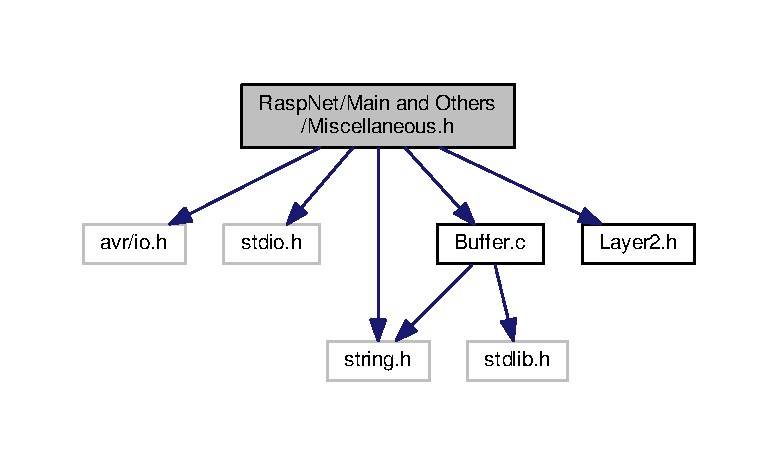
\includegraphics[width=350pt]{Miscellaneous_8h__incl}
\end{center}
\end{figure}
This graph shows which files directly or indirectly include this file\+:
\nopagebreak
\begin{figure}[H]
\begin{center}
\leavevmode
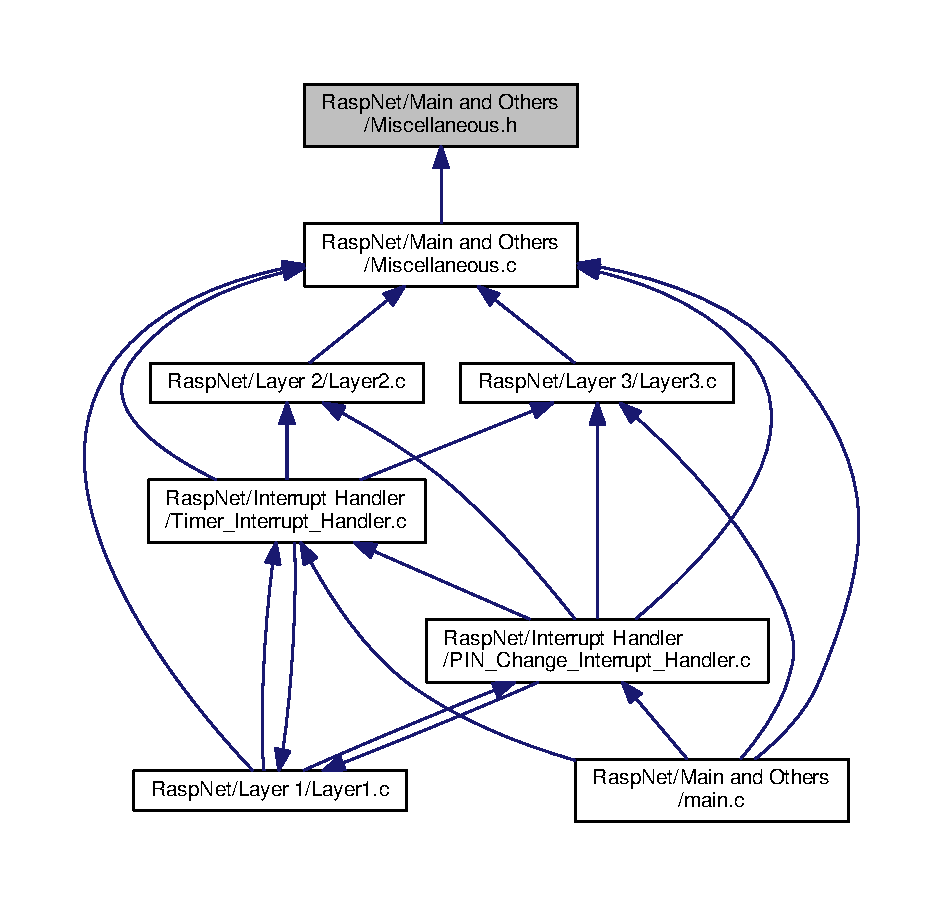
\includegraphics[width=350pt]{Miscellaneous_8h__dep__incl}
\end{center}
\end{figure}
\subsection*{Functions}
\begin{DoxyCompactItemize}
\item 
void \hyperlink{Miscellaneous_8h_ade3319d0c8a73744f47a483a8816cabe}{uart\+\_\+transmission} (unsigned char character)
\begin{DoxyCompactList}\small\item\em Display a single character in the minicom command line interface. \end{DoxyCompactList}\item 
void \hyperlink{Miscellaneous_8h_afac087d6e168f5fc2cd8994eb07eadb2}{show\+Log} (char msg\mbox{[}$\,$\mbox{]})
\begin{DoxyCompactList}\small\item\em Display message consists of string. \end{DoxyCompactList}\item 
int \hyperlink{Miscellaneous_8h_a3c3d2514913829c2be8324680f0987b9}{read\+\_\+8\+\_\+bit} (uint8\+\_\+t bits, int pos)
\begin{DoxyCompactList}\small\item\em Read from 8 bit unsigned integer. \end{DoxyCompactList}\item 
int \hyperlink{Miscellaneous_8h_a027b54125044a7b75a94ebdfef27ab46}{read\+\_\+32\+\_\+bit} (uint32\+\_\+t bits, int pos)
\begin{DoxyCompactList}\small\item\em Read from 32 bit unsigned integer. \end{DoxyCompactList}\item 
uint8\+\_\+t \hyperlink{Miscellaneous_8h_af81f6965e50b219ff38ea272019bac1f}{write\+\_\+8\+\_\+bit} (uint8\+\_\+t value, int pos, int value\+\_\+to\+\_\+write)
\begin{DoxyCompactList}\small\item\em Write in 8 bit unsigned integer. \end{DoxyCompactList}\item 
uint32\+\_\+t \hyperlink{Miscellaneous_8h_a864fd2a5d36c61fdc91090a497784b55}{write\+\_\+32\+\_\+bit} (uint32\+\_\+t value, int pos, int value\+\_\+to\+\_\+write)
\begin{DoxyCompactList}\small\item\em Write in 32 bit unsigned integer. \end{DoxyCompactList}\item 
int \hyperlink{Miscellaneous_8h_ad063f3ce115eb187d5cbb6fd2b00c0e6}{compare\+\_\+preamble} (uint8\+\_\+t a, uint8\+\_\+t b)
\begin{DoxyCompactList}\small\item\em Compare between received preamble and predefined preamble. \end{DoxyCompactList}\item 
int \hyperlink{Miscellaneous_8h_a7ea454e652a249ba5f17f6233e65887a}{compare\+\_\+crc} (uint32\+\_\+t a, uint32\+\_\+t b)
\begin{DoxyCompactList}\small\item\em Compare between received C\+RC and generated C\+RC from payload. \end{DoxyCompactList}\item 
void \hyperlink{Miscellaneous_8h_a9ea1d4b6a27b5caa55c150b2ba17983a}{show\+\_\+payload} (uint8\+\_\+t $\ast$data, uint8\+\_\+t length)
\begin{DoxyCompactList}\small\item\em Display payload message. \end{DoxyCompactList}\end{DoxyCompactItemize}


\subsection{Function Documentation}
\index{Miscellaneous.\+h@{Miscellaneous.\+h}!compare\+\_\+crc@{compare\+\_\+crc}}
\index{compare\+\_\+crc@{compare\+\_\+crc}!Miscellaneous.\+h@{Miscellaneous.\+h}}
\subsubsection[{\texorpdfstring{compare\+\_\+crc(uint32\+\_\+t a, uint32\+\_\+t b)}{compare_crc(uint32_t a, uint32_t b)}}]{\setlength{\rightskip}{0pt plus 5cm}int compare\+\_\+crc (
\begin{DoxyParamCaption}
\item[{uint32\+\_\+t}]{a, }
\item[{uint32\+\_\+t}]{b}
\end{DoxyParamCaption}
)}\hypertarget{Miscellaneous_8h_a7ea454e652a249ba5f17f6233e65887a}{}\label{Miscellaneous_8h_a7ea454e652a249ba5f17f6233e65887a}


Compare between received C\+RC and generated C\+RC from payload. 


\begin{DoxyParams}{Parameters}
{\em a} & 32 bit unsigned integer, which is generated from the payload \\
\hline
{\em b} & 32 bit unsigned integer, which is received \\
\hline
\end{DoxyParams}
\begin{DoxyReturn}{Returns}
int data, which is 1 if match otherwise, 0 if does not match 
\end{DoxyReturn}
$<$ Bit compare using X\+OR

$<$ O X\+OR 1 = 1

$<$ O X\+OR 0 = 0, 1 X\+OR 1 = 0 
\begin{DoxyCode}
132                                         \{
133     \textcolor{keywordflow}{if}(!(a^b)) \{    
134         \textcolor{keywordflow}{return} 1;   
135     \}
136     \textcolor{keywordflow}{else} \{
137         \textcolor{keywordflow}{return} 0;   
138     \}
139 \}
\end{DoxyCode}
\index{Miscellaneous.\+h@{Miscellaneous.\+h}!compare\+\_\+preamble@{compare\+\_\+preamble}}
\index{compare\+\_\+preamble@{compare\+\_\+preamble}!Miscellaneous.\+h@{Miscellaneous.\+h}}
\subsubsection[{\texorpdfstring{compare\+\_\+preamble(uint8\+\_\+t a, uint8\+\_\+t b)}{compare_preamble(uint8_t a, uint8_t b)}}]{\setlength{\rightskip}{0pt plus 5cm}int compare\+\_\+preamble (
\begin{DoxyParamCaption}
\item[{uint8\+\_\+t}]{a, }
\item[{uint8\+\_\+t}]{b}
\end{DoxyParamCaption}
)}\hypertarget{Miscellaneous_8h_ad063f3ce115eb187d5cbb6fd2b00c0e6}{}\label{Miscellaneous_8h_ad063f3ce115eb187d5cbb6fd2b00c0e6}


Compare between received preamble and predefined preamble. 


\begin{DoxyParams}{Parameters}
{\em a} & 8 bit unsigned integer, which is predefined \\
\hline
{\em b} & 8 bit unsigned integer, which is received \\
\hline
\end{DoxyParams}
\begin{DoxyReturn}{Returns}
int data, which is 1 if match otherwise, 0 if does not match 
\end{DoxyReturn}
$<$ Bit compare using X\+OR

$<$ O X\+OR 1 = 1

$<$ O X\+OR 0 = 0, 1 X\+OR 1 = 0 
\begin{DoxyCode}
71                                            \{
72     \textcolor{keywordflow}{if}(!(a^b)) \{                 
73         \textcolor{keywordflow}{return} 1;                
74     \}
75     \textcolor{keywordflow}{else} \{
76         \textcolor{keywordflow}{return} 0;                
77     \}
78 \}
\end{DoxyCode}
\index{Miscellaneous.\+h@{Miscellaneous.\+h}!read\+\_\+32\+\_\+bit@{read\+\_\+32\+\_\+bit}}
\index{read\+\_\+32\+\_\+bit@{read\+\_\+32\+\_\+bit}!Miscellaneous.\+h@{Miscellaneous.\+h}}
\subsubsection[{\texorpdfstring{read\+\_\+32\+\_\+bit(uint32\+\_\+t bits, int pos)}{read_32_bit(uint32_t bits, int pos)}}]{\setlength{\rightskip}{0pt plus 5cm}int read\+\_\+32\+\_\+bit (
\begin{DoxyParamCaption}
\item[{uint32\+\_\+t}]{bits, }
\item[{int}]{pos}
\end{DoxyParamCaption}
)}\hypertarget{Miscellaneous_8h_a027b54125044a7b75a94ebdfef27ab46}{}\label{Miscellaneous_8h_a027b54125044a7b75a94ebdfef27ab46}


Read from 32 bit unsigned integer. 


\begin{DoxyParams}{Parameters}
{\em bits} & The 32 bit integer to read to \\
\hline
{\em pos} & Read bit at particular position \\
\hline
\end{DoxyParams}
\begin{DoxyReturn}{Returns}
int data which are 1 or 0 
\end{DoxyReturn}
$<$ Casting and left shift 
\begin{DoxyCode}
21                                         \{
22     uint32\_t mask;
23     mask=((uint32\_t)0x00000001) << pos; 
24     \textcolor{keywordflow}{if}(bits&mask) \{
25         \textcolor{keywordflow}{return} 1;
26     \}
27     \textcolor{keywordflow}{else} \{
28         \textcolor{keywordflow}{return} 0;
29     \}
30 \}
\end{DoxyCode}
\index{Miscellaneous.\+h@{Miscellaneous.\+h}!read\+\_\+8\+\_\+bit@{read\+\_\+8\+\_\+bit}}
\index{read\+\_\+8\+\_\+bit@{read\+\_\+8\+\_\+bit}!Miscellaneous.\+h@{Miscellaneous.\+h}}
\subsubsection[{\texorpdfstring{read\+\_\+8\+\_\+bit(uint8\+\_\+t bits, int pos)}{read_8_bit(uint8_t bits, int pos)}}]{\setlength{\rightskip}{0pt plus 5cm}int read\+\_\+8\+\_\+bit (
\begin{DoxyParamCaption}
\item[{uint8\+\_\+t}]{bits, }
\item[{int}]{pos}
\end{DoxyParamCaption}
)}\hypertarget{Miscellaneous_8h_a3c3d2514913829c2be8324680f0987b9}{}\label{Miscellaneous_8h_a3c3d2514913829c2be8324680f0987b9}


Read from 8 bit unsigned integer. 


\begin{DoxyParams}{Parameters}
{\em bits} & The 8 bit integer to read to \\
\hline
{\em pos} & Read bit at particular position \\
\hline
\end{DoxyParams}
\begin{DoxyReturn}{Returns}
int data 1 or 0
\end{DoxyReturn}
$<$ allows to include header file when needed otherwise ignore $<$ Left shift based on pos value

$<$ Logical \& to check bit at particular position 
\begin{DoxyCode}
11                                       \{
12     pos=(1<<pos); 
13     \textcolor{keywordflow}{if}(bits&pos) \{ 
14         \textcolor{keywordflow}{return} 1;
15     \}
16     \textcolor{keywordflow}{else} \{
17         \textcolor{keywordflow}{return} 0;
18     \}
19 \}
\end{DoxyCode}
\index{Miscellaneous.\+h@{Miscellaneous.\+h}!show\+\_\+payload@{show\+\_\+payload}}
\index{show\+\_\+payload@{show\+\_\+payload}!Miscellaneous.\+h@{Miscellaneous.\+h}}
\subsubsection[{\texorpdfstring{show\+\_\+payload(uint8\+\_\+t $\ast$data, uint8\+\_\+t length)}{show_payload(uint8_t *data, uint8_t length)}}]{\setlength{\rightskip}{0pt plus 5cm}void show\+\_\+payload (
\begin{DoxyParamCaption}
\item[{uint8\+\_\+t $\ast$}]{data, }
\item[{uint8\+\_\+t}]{length}
\end{DoxyParamCaption}
)}\hypertarget{Miscellaneous_8h_a9ea1d4b6a27b5caa55c150b2ba17983a}{}\label{Miscellaneous_8h_a9ea1d4b6a27b5caa55c150b2ba17983a}


Display payload message. 


\begin{DoxyParams}{Parameters}
{\em data} & 8 bit unsigned character array \\
\hline
{\em length} & Length of the payload \\
\hline
\end{DoxyParams}
\begin{DoxyReturn}{Returns}
void nothing has to return 
\end{DoxyReturn}
$<$ Iterate over every element of the array

$<$ Read from the M\+SB

$<$ Display 1

$<$ Display 0 
\begin{DoxyCode}
113                                                  \{
114     \textcolor{keywordtype}{int} i,j;
115     \hyperlink{Miscellaneous_8h_ade3319d0c8a73744f47a483a8816cabe}{uart\_transmission}(\textcolor{charliteral}{'\(\backslash\)n'});
116     \hyperlink{Miscellaneous_8h_ade3319d0c8a73744f47a483a8816cabe}{uart\_transmission}(\textcolor{charliteral}{'\(\backslash\)r'});
117     \textcolor{keywordflow}{for}(i=0; i<length/8; i++) \{ 
118         \textcolor{keywordflow}{for}(j=7; j>=0; j--) \{ 
119             \textcolor{keywordflow}{if}(\hyperlink{Miscellaneous_8c_a027b54125044a7b75a94ebdfef27ab46}{read\_32\_bit}(data[i],j)) \{
120                 \hyperlink{Miscellaneous_8h_ade3319d0c8a73744f47a483a8816cabe}{uart\_transmission}(\textcolor{charliteral}{'1'}); 
121             \}
122             \textcolor{keywordflow}{else} \{
123                 \hyperlink{Miscellaneous_8h_ade3319d0c8a73744f47a483a8816cabe}{uart\_transmission}(\textcolor{charliteral}{'0'}); 
124             \}
125         \}
126     \}
127     \hyperlink{Miscellaneous_8h_ade3319d0c8a73744f47a483a8816cabe}{uart\_transmission}(\textcolor{charliteral}{'\(\backslash\)n'});
128     \hyperlink{Miscellaneous_8h_ade3319d0c8a73744f47a483a8816cabe}{uart\_transmission}(\textcolor{charliteral}{'\(\backslash\)r'});
129 \}
\end{DoxyCode}
\index{Miscellaneous.\+h@{Miscellaneous.\+h}!show\+Log@{show\+Log}}
\index{show\+Log@{show\+Log}!Miscellaneous.\+h@{Miscellaneous.\+h}}
\subsubsection[{\texorpdfstring{show\+Log(char msg[])}{showLog(char msg[])}}]{\setlength{\rightskip}{0pt plus 5cm}void show\+Log (
\begin{DoxyParamCaption}
\item[{char}]{msg\mbox{[}$\,$\mbox{]}}
\end{DoxyParamCaption}
)}\hypertarget{Miscellaneous_8h_afac087d6e168f5fc2cd8994eb07eadb2}{}\label{Miscellaneous_8h_afac087d6e168f5fc2cd8994eb07eadb2}


Display message consists of string. 


\begin{DoxyParams}{Parameters}
{\em msg} & Message for display in the minicom command line interface \\
\hline
{\em void} & nothing has to return from this function \\
\hline
\end{DoxyParams}
$<$ Display message until getting the null value

$<$ U\+A\+RT function to display message 
\begin{DoxyCode}
60                          \{
61     \textcolor{keywordtype}{int} i=0;
62     \hyperlink{Miscellaneous_8h_ade3319d0c8a73744f47a483a8816cabe}{uart\_transmission}(\textcolor{charliteral}{'\(\backslash\)r'});
63     \hyperlink{Miscellaneous_8h_ade3319d0c8a73744f47a483a8816cabe}{uart\_transmission}(\textcolor{charliteral}{'\(\backslash\)n'});
64     \textcolor{keywordflow}{for}(i=0; msg[i]!=\textcolor{charliteral}{'\(\backslash\)0'}; i++) \{ 
65         \hyperlink{Miscellaneous_8h_ade3319d0c8a73744f47a483a8816cabe}{uart\_transmission}(msg[i]);
67     \}
68 
69 \}
\end{DoxyCode}
\index{Miscellaneous.\+h@{Miscellaneous.\+h}!uart\+\_\+transmission@{uart\+\_\+transmission}}
\index{uart\+\_\+transmission@{uart\+\_\+transmission}!Miscellaneous.\+h@{Miscellaneous.\+h}}
\subsubsection[{\texorpdfstring{uart\+\_\+transmission(unsigned char character)}{uart_transmission(unsigned char character)}}]{\setlength{\rightskip}{0pt plus 5cm}void uart\+\_\+transmission (
\begin{DoxyParamCaption}
\item[{unsigned char}]{character}
\end{DoxyParamCaption}
)}\hypertarget{Miscellaneous_8h_ade3319d0c8a73744f47a483a8816cabe}{}\label{Miscellaneous_8h_ade3319d0c8a73744f47a483a8816cabe}


Display a single character in the minicom command line interface. 

$<$ allows to include header file when needed otherwise ignore
\begin{DoxyParams}{Parameters}
{\em character} & Character for display in the minicom command line interface \\
\hline
\end{DoxyParams}
\begin{DoxyReturn}{Returns}
void nothing has to return from this function 
\end{DoxyReturn}
$<$ Wait until the register is free

$<$write the new data in Transmit Buffer (U\+DR) 
\begin{DoxyCode}
6                                                \{
7     \textcolor{keywordflow}{while}(!(UCSR0A & (1<<UDRE0))); 
8     UDR0= send\_data; 
9 \}
\end{DoxyCode}
\index{Miscellaneous.\+h@{Miscellaneous.\+h}!write\+\_\+32\+\_\+bit@{write\+\_\+32\+\_\+bit}}
\index{write\+\_\+32\+\_\+bit@{write\+\_\+32\+\_\+bit}!Miscellaneous.\+h@{Miscellaneous.\+h}}
\subsubsection[{\texorpdfstring{write\+\_\+32\+\_\+bit(uint32\+\_\+t value, int pos, int value\+\_\+to\+\_\+write)}{write_32_bit(uint32_t value, int pos, int value_to_write)}}]{\setlength{\rightskip}{0pt plus 5cm}uint32\+\_\+t write\+\_\+32\+\_\+bit (
\begin{DoxyParamCaption}
\item[{uint32\+\_\+t}]{value, }
\item[{int}]{pos, }
\item[{int}]{value\+\_\+to\+\_\+write}
\end{DoxyParamCaption}
)}\hypertarget{Miscellaneous_8h_a864fd2a5d36c61fdc91090a497784b55}{}\label{Miscellaneous_8h_a864fd2a5d36c61fdc91090a497784b55}


Write in 32 bit unsigned integer. 


\begin{DoxyParams}{Parameters}
{\em value} & The 32 bit integer to write to \\
\hline
{\em pos} & Write at particular position \\
\hline
{\em value\+\_\+to\+\_\+write} & int data which are 0 or 1 \\
\hline
\end{DoxyParams}
\begin{DoxyReturn}{Returns}
uint32\+\_\+t data 
\end{DoxyReturn}
$<$ Casting and left shift

$<$ Casting and left shift

$<$ When need to write 1

$<$ Logical OR to set bit at particular position

$<$ When need to write 0 
\begin{DoxyCode}
46                                                                   \{
47     uint32\_t mask1,mask2;
48     mask1=((uint32\_t)0x00000001) << pos; 
49     mask2=((uint32\_t)0x00000000) << pos; 
50     \textcolor{keywordflow}{if}(value\_to\_write==1) \{              
51         value=value|mask1;               
52     \}
53     \textcolor{keywordflow}{else} \{
54         value=value|mask2;               
55     \}
56 
57     \textcolor{keywordflow}{return} value;
58 \}
\end{DoxyCode}
\index{Miscellaneous.\+h@{Miscellaneous.\+h}!write\+\_\+8\+\_\+bit@{write\+\_\+8\+\_\+bit}}
\index{write\+\_\+8\+\_\+bit@{write\+\_\+8\+\_\+bit}!Miscellaneous.\+h@{Miscellaneous.\+h}}
\subsubsection[{\texorpdfstring{write\+\_\+8\+\_\+bit(uint8\+\_\+t value, int pos, int value\+\_\+to\+\_\+write)}{write_8_bit(uint8_t value, int pos, int value_to_write)}}]{\setlength{\rightskip}{0pt plus 5cm}uint8\+\_\+t write\+\_\+8\+\_\+bit (
\begin{DoxyParamCaption}
\item[{uint8\+\_\+t}]{value, }
\item[{int}]{pos, }
\item[{int}]{value\+\_\+to\+\_\+write}
\end{DoxyParamCaption}
)}\hypertarget{Miscellaneous_8h_af81f6965e50b219ff38ea272019bac1f}{}\label{Miscellaneous_8h_af81f6965e50b219ff38ea272019bac1f}


Write in 8 bit unsigned integer. 


\begin{DoxyParams}{Parameters}
{\em value} & The 8 bit integer to write to \\
\hline
{\em pos} & Write at particular position \\
\hline
{\em value\+\_\+to\+\_\+write} & int data which are 0 or 1 \\
\hline
\end{DoxyParams}
\begin{DoxyReturn}{Returns}
uint8\+\_\+t data 
\end{DoxyReturn}
$<$ Casting and left shift

$<$ Casting and left shift

$<$ When need to write 1

$<$ Logical OR to set bit at particular position

$<$ When need to write 0 
\begin{DoxyCode}
32                                                                \{
33     uint8\_t mask1,mask2;
34     mask1=((uint8\_t)1)<<pos; 
35     mask2=((uint8\_t)0)<<pos; 
36     \textcolor{keywordflow}{if}(value\_to\_write==1) \{  
37         value=value|mask1;   
38     \}
39     \textcolor{keywordflow}{else} \{
40         value=value|mask2;  
41     \}
42 
43     \textcolor{keywordflow}{return} value;
44 \}
\end{DoxyCode}

\hypertarget{UART__Handler_8c}{}\section{Rasp\+Net/\+U\+A\+RT handler/\+U\+A\+R\+T\+\_\+\+Handler.c File Reference}
\label{UART__Handler_8c}\index{Rasp\+Net/\+U\+A\+R\+T handler/\+U\+A\+R\+T\+\_\+\+Handler.\+c@{Rasp\+Net/\+U\+A\+R\+T handler/\+U\+A\+R\+T\+\_\+\+Handler.\+c}}
{\ttfamily \#include $<$avr/io.\+h$>$}\\*
{\ttfamily \#include \char`\"{}U\+A\+R\+T\+\_\+\+Handler.\+h\char`\"{}}\\*
Include dependency graph for U\+A\+R\+T\+\_\+\+Handler.\+c\+:
\nopagebreak
\begin{figure}[H]
\begin{center}
\leavevmode
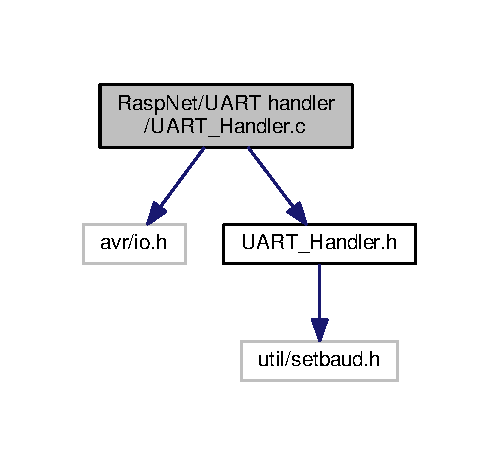
\includegraphics[width=240pt]{UART__Handler_8c__incl}
\end{center}
\end{figure}
This graph shows which files directly or indirectly include this file\+:
\nopagebreak
\begin{figure}[H]
\begin{center}
\leavevmode
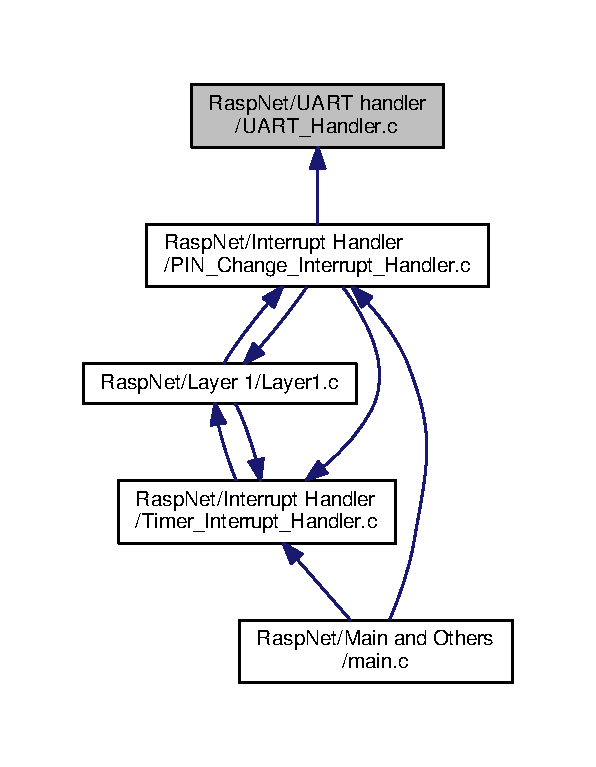
\includegraphics[width=286pt]{UART__Handler_8c__dep__incl}
\end{center}
\end{figure}
\subsection*{Functions}
\begin{DoxyCompactItemize}
\item 
void \hyperlink{UART__Handler_8c_aeef44b01b53c54757fcdd09b859a52a4}{uart\+\_\+transmission} (unsigned char send\+\_\+data)
\begin{DoxyCompactList}\small\item\em Display a single character in the minicom command line interface. \end{DoxyCompactList}\item 
unsigned char \hyperlink{UART__Handler_8c_a66dc17a92418b1104efccc95f7e7ec3f}{uart\+\_\+receive} ()
\begin{DoxyCompactList}\small\item\em U\+A\+RT receive message\+: receive message. \end{DoxyCompactList}\end{DoxyCompactItemize}


\subsection{Function Documentation}
\index{U\+A\+R\+T\+\_\+\+Handler.\+c@{U\+A\+R\+T\+\_\+\+Handler.\+c}!uart\+\_\+receive@{uart\+\_\+receive}}
\index{uart\+\_\+receive@{uart\+\_\+receive}!U\+A\+R\+T\+\_\+\+Handler.\+c@{U\+A\+R\+T\+\_\+\+Handler.\+c}}
\subsubsection[{\texorpdfstring{uart\+\_\+receive()}{uart_receive()}}]{\setlength{\rightskip}{0pt plus 5cm}unsigned char uart\+\_\+receive (
\begin{DoxyParamCaption}
{}
\end{DoxyParamCaption}
)}\hypertarget{UART__Handler_8c_a66dc17a92418b1104efccc95f7e7ec3f}{}\label{UART__Handler_8c_a66dc17a92418b1104efccc95f7e7ec3f}


U\+A\+RT receive message\+: receive message. 

\begin{DoxyReturn}{Returns}
unsigned character, which is received from U\+A\+RT transmission 
\end{DoxyReturn}
$<$ Wait until the data is received 
\begin{DoxyCode}
11                             \{
12     \textcolor{keywordflow}{while}(!(UCSR0A & (1<<RXC0))); 
13     \textcolor{keywordflow}{return} UDR0; \textcolor{comment}{// UDR return 8 bit}
14  \}
\end{DoxyCode}
\index{U\+A\+R\+T\+\_\+\+Handler.\+c@{U\+A\+R\+T\+\_\+\+Handler.\+c}!uart\+\_\+transmission@{uart\+\_\+transmission}}
\index{uart\+\_\+transmission@{uart\+\_\+transmission}!U\+A\+R\+T\+\_\+\+Handler.\+c@{U\+A\+R\+T\+\_\+\+Handler.\+c}}
\subsubsection[{\texorpdfstring{uart\+\_\+transmission(unsigned char send\+\_\+data)}{uart_transmission(unsigned char send_data)}}]{\setlength{\rightskip}{0pt plus 5cm}void uart\+\_\+transmission (
\begin{DoxyParamCaption}
\item[{unsigned char}]{character}
\end{DoxyParamCaption}
)}\hypertarget{UART__Handler_8c_aeef44b01b53c54757fcdd09b859a52a4}{}\label{UART__Handler_8c_aeef44b01b53c54757fcdd09b859a52a4}


Display a single character in the minicom command line interface. 

U\+A\+RT transmission message\+: to display message.

$<$ allows to include header file when needed otherwise ignore
\begin{DoxyParams}{Parameters}
{\em character} & Character for display in the minicom command line interface \\
\hline
\end{DoxyParams}
\begin{DoxyReturn}{Returns}
void nothing has to return from this function 
\end{DoxyReturn}
$<$ Wait until the register is free

$<$write the new data in Transmit Buffer (U\+DR) 
\begin{DoxyCode}
6                                                \{
7     \textcolor{keywordflow}{while}(!(UCSR0A & (1<<UDRE0))); 
8     UDR0= send\_data; 
9 \}
\end{DoxyCode}

\hypertarget{UART__Handler_8h}{}\section{Rasp\+Net/\+U\+A\+RT handler/\+U\+A\+R\+T\+\_\+\+Handler.h File Reference}
\label{UART__Handler_8h}\index{Rasp\+Net/\+U\+A\+R\+T handler/\+U\+A\+R\+T\+\_\+\+Handler.\+h@{Rasp\+Net/\+U\+A\+R\+T handler/\+U\+A\+R\+T\+\_\+\+Handler.\+h}}
{\ttfamily \#include $<$util/setbaud.\+h$>$}\\*
Include dependency graph for U\+A\+R\+T\+\_\+\+Handler.\+h\+:
\nopagebreak
\begin{figure}[H]
\begin{center}
\leavevmode
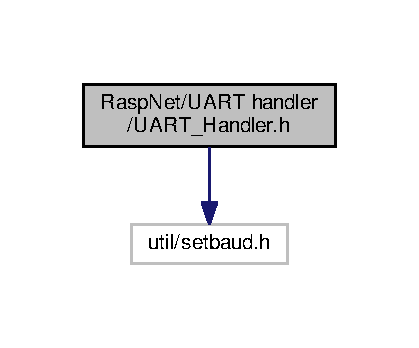
\includegraphics[width=201pt]{UART__Handler_8h__incl}
\end{center}
\end{figure}
This graph shows which files directly or indirectly include this file\+:
\nopagebreak
\begin{figure}[H]
\begin{center}
\leavevmode
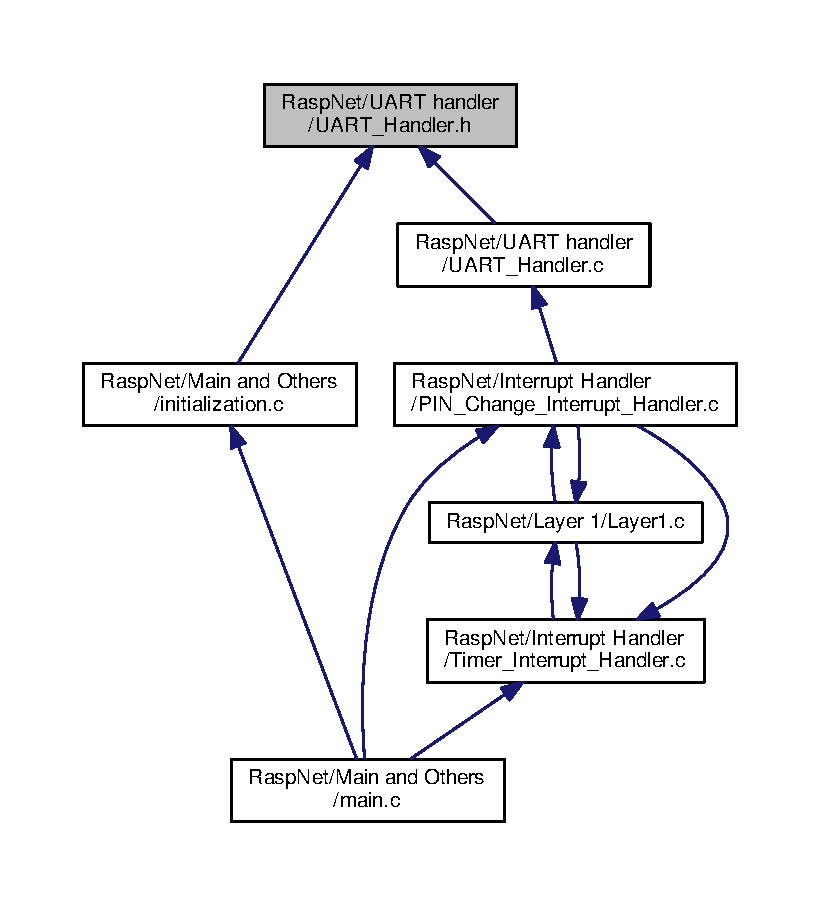
\includegraphics[width=350pt]{UART__Handler_8h__dep__incl}
\end{center}
\end{figure}
\subsection*{Macros}
\begin{DoxyCompactItemize}
\item 
\#define \hyperlink{UART__Handler_8h_a62634036639f88eece6fbf226b45f84b}{B\+A\+UD}~19200\+UL
\item 
\#define \hyperlink{UART__Handler_8h_a734bbab06e1a9fd2e5522db0221ff6e3}{B\+A\+U\+D\+R\+A\+TE}~(\hyperlink{main_8c_a43bafb28b29491ec7f871319b5a3b2f8}{F\+\_\+\+C\+PU}/(16$\ast$\hyperlink{UART__Handler_8h_a62634036639f88eece6fbf226b45f84b}{B\+A\+UD})-\/1)
\end{DoxyCompactItemize}
\subsection*{Functions}
\begin{DoxyCompactItemize}
\item 
void \hyperlink{UART__Handler_8h_ade3319d0c8a73744f47a483a8816cabe}{uart\+\_\+transmission} (unsigned char character)
\begin{DoxyCompactList}\small\item\em U\+A\+RT transmission message\+: to display message. \end{DoxyCompactList}\item 
unsigned char \hyperlink{UART__Handler_8h_a66dc17a92418b1104efccc95f7e7ec3f}{uart\+\_\+receive} ()
\begin{DoxyCompactList}\small\item\em U\+A\+RT receive message\+: receive message. \end{DoxyCompactList}\end{DoxyCompactItemize}


\subsection{Macro Definition Documentation}
\index{U\+A\+R\+T\+\_\+\+Handler.\+h@{U\+A\+R\+T\+\_\+\+Handler.\+h}!B\+A\+UD@{B\+A\+UD}}
\index{B\+A\+UD@{B\+A\+UD}!U\+A\+R\+T\+\_\+\+Handler.\+h@{U\+A\+R\+T\+\_\+\+Handler.\+h}}
\subsubsection[{\texorpdfstring{B\+A\+UD}{BAUD}}]{\setlength{\rightskip}{0pt plus 5cm}\#define B\+A\+UD~19200\+UL}\hypertarget{UART__Handler_8h_a62634036639f88eece6fbf226b45f84b}{}\label{UART__Handler_8h_a62634036639f88eece6fbf226b45f84b}
$<$ allows to include header file when needed otherwise ignore \index{U\+A\+R\+T\+\_\+\+Handler.\+h@{U\+A\+R\+T\+\_\+\+Handler.\+h}!B\+A\+U\+D\+R\+A\+TE@{B\+A\+U\+D\+R\+A\+TE}}
\index{B\+A\+U\+D\+R\+A\+TE@{B\+A\+U\+D\+R\+A\+TE}!U\+A\+R\+T\+\_\+\+Handler.\+h@{U\+A\+R\+T\+\_\+\+Handler.\+h}}
\subsubsection[{\texorpdfstring{B\+A\+U\+D\+R\+A\+TE}{BAUDRATE}}]{\setlength{\rightskip}{0pt plus 5cm}\#define B\+A\+U\+D\+R\+A\+TE~({\bf F\+\_\+\+C\+PU}/(16$\ast${\bf B\+A\+UD})-\/1)}\hypertarget{UART__Handler_8h_a734bbab06e1a9fd2e5522db0221ff6e3}{}\label{UART__Handler_8h_a734bbab06e1a9fd2e5522db0221ff6e3}


\subsection{Function Documentation}
\index{U\+A\+R\+T\+\_\+\+Handler.\+h@{U\+A\+R\+T\+\_\+\+Handler.\+h}!uart\+\_\+receive@{uart\+\_\+receive}}
\index{uart\+\_\+receive@{uart\+\_\+receive}!U\+A\+R\+T\+\_\+\+Handler.\+h@{U\+A\+R\+T\+\_\+\+Handler.\+h}}
\subsubsection[{\texorpdfstring{uart\+\_\+receive()}{uart_receive()}}]{\setlength{\rightskip}{0pt plus 5cm}unsigned char uart\+\_\+receive (
\begin{DoxyParamCaption}
{}
\end{DoxyParamCaption}
)}\hypertarget{UART__Handler_8h_a66dc17a92418b1104efccc95f7e7ec3f}{}\label{UART__Handler_8h_a66dc17a92418b1104efccc95f7e7ec3f}


U\+A\+RT receive message\+: receive message. 

\begin{DoxyReturn}{Returns}
unsigned character, which is received from U\+A\+RT transmission 
\end{DoxyReturn}
$<$ Wait until the data is received 
\begin{DoxyCode}
11                             \{
12     \textcolor{keywordflow}{while}(!(UCSR0A & (1<<RXC0))); 
13     \textcolor{keywordflow}{return} UDR0; \textcolor{comment}{// UDR return 8 bit}
14  \}
\end{DoxyCode}
\index{U\+A\+R\+T\+\_\+\+Handler.\+h@{U\+A\+R\+T\+\_\+\+Handler.\+h}!uart\+\_\+transmission@{uart\+\_\+transmission}}
\index{uart\+\_\+transmission@{uart\+\_\+transmission}!U\+A\+R\+T\+\_\+\+Handler.\+h@{U\+A\+R\+T\+\_\+\+Handler.\+h}}
\subsubsection[{\texorpdfstring{uart\+\_\+transmission(unsigned char character)}{uart_transmission(unsigned char character)}}]{\setlength{\rightskip}{0pt plus 5cm}void uart\+\_\+transmission (
\begin{DoxyParamCaption}
\item[{unsigned char}]{character}
\end{DoxyParamCaption}
)}\hypertarget{UART__Handler_8h_ade3319d0c8a73744f47a483a8816cabe}{}\label{UART__Handler_8h_ade3319d0c8a73744f47a483a8816cabe}


U\+A\+RT transmission message\+: to display message. 


\begin{DoxyParams}{Parameters}
{\em character} & Unsigned integer to display \\
\hline
\end{DoxyParams}
\begin{DoxyReturn}{Returns}
void nothing has to be returned
\end{DoxyReturn}
U\+A\+RT transmission message\+: to display message.

$<$ allows to include header file when needed otherwise ignore
\begin{DoxyParams}{Parameters}
{\em character} & Character for display in the minicom command line interface \\
\hline
\end{DoxyParams}
\begin{DoxyReturn}{Returns}
void nothing has to return from this function 
\end{DoxyReturn}
$<$ Wait until the register is free

$<$write the new data in Transmit Buffer (U\+DR) 
\begin{DoxyCode}
6                                                \{
7     \textcolor{keywordflow}{while}(!(UCSR0A & (1<<UDRE0))); 
8     UDR0= send\_data; 
9 \}
\end{DoxyCode}

\hypertarget{README_8md}{}\section{R\+E\+A\+D\+M\+E.\+md File Reference}
\label{README_8md}\index{R\+E\+A\+D\+M\+E.\+md@{R\+E\+A\+D\+M\+E.\+md}}

%--- End generated contents ---

% Index
\backmatter
\newpage
\phantomsection
\clearemptydoublepage
\addcontentsline{toc}{chapter}{Index}
\printindex

\end{document}
